\chapter{Rapid programmatic agonist delivery to a neuronal microculture}
\label{chap:microculturePulses}
\section{Introduction}
In this chapter we combine all the components developed in previous chapters to construct a system with the capability of second-scale agonist pulsing over an entire neuronal microculture. To this end, we  start by providing a new design for microwell devices, taking into account the lessons learnt from the pilot design put forward in section \ref{sec:devices:microcultures}, and growing neuronal microcultures in them. Specific further tweaks to the protocol which were needed to achieve satisfactory results are discussed as well. Secondly, we will test the device's pulsing performance by visualizing the agonist time course using a fluorescent marker. We further show that the pulsing performance can be accurately predicted using a numerical fluid dynamics simulation in Comsol. Such models could assist in future design of similar devices to meet bespoke criteria. We further test the ability to obtain a biological response from the cultures grown in the microwell devices at the required time scales through pulsing of glutamate and recording the neuronal activation on microelectrode arrays. Finally, we use the developed system to apply dopamine pulses to the microcultures while inducing evoked activity using electrical stimulations. By running these final experiments we effectively realize the Izhikevic thought experiment (section \ref{sec:introduction:izi}) and achieve the declared goal of this Ph.D.

\section{Fabrication and establishment of long term neuronal microcultures}
\label{sec:pulses:microcultures}
The devices were based on a 2-layer design comprising a PDMS microwell layer and a tape-based flow layer. The design is illustrated in figure \ref{fig:pulses:circularIllustration} and the fabrication process is described next. The PDMS layers used in this section were manufactured using thin film spinning (section \ref{sec:methods:fabrication}, either \(120\) or \(80 \mu m\) thick). They were based on the design introduced in section \ref{sec:devices:microcultures} which includes a main experimental microwell together with a large rectangular support well. The distances were selected so that the support well would be placed on top of the internal reference electrode of the MEA to allow it contact with the media. The microwell was created using a \(0.8 mm\) biopsy punch whereas the support well was cut manually using a scalpel. In this manual procedure, the dimensions were adhered to by placing the cured PDMS sheet on top of a printout of the layer design for reference. The earlier pilot study showed that microcultures exhibit a high rate of degeneration, depending on their size, and that the largest microwell sizes used in that study, \(400\times 400 \mu m^{2}\), were able to match the viability of macrocultures. The punched microwells in the new design were of average diameter of \(675 \mu m\) placing them further in the safe zone. The flow layer was cut out of a \(50 \mu m\) silicone transfer tape (section \ref{sec:methods:fabrication}). The assembly process started by joining the flow layer to a pre-cured PDMS bulk and punching of the ports. All elements were then heat sterilized in \(120\degree C\). Next, the microwell layer was placed on top of a commercial MEA pre-coated with PEI (section \ref{sec:methods:surface}) while aligning the microwell and the support well with the central recording and the reference electrode, respectively. A reversible hydrophobic bond is generated when PDMS is put in contact with a glass surface. This was followed by joining of the flow layer (and the PDMS bulk) with the top surface of the microwell layer while making sure that the microwell is positioned as close as possible to the apex of the channel. The device was completed by gluing a glass chamber around the device to hold the growth media (figure \ref{fig:pulses:circularIllustration} bottom images). The devices were seeded by pushing \(2 \mu L\) of seeding suspension at a density of \(12\times 10^{6} cells\cdot ml^{-1}\). The density was found to play a significant role which will further addressed later. After 1 day of incubation the devices were flushed to remove excess cells from the top of the PDMS sheet. In contrast with how the microcultures were prepared in section \ref{sec:devices:microcultures}, the surface-then-bonding approach used here guaranteed that only the microwell surface was cell adhesive so the cells on top of the PDMS sheet were not strongly attached. This allowed us to use a more delicate flushing routine to avoid any removal of cells from the microwell. This proceeded by using a syringe driver to apply a controlled flow rate of \(50 \mu L\cdot min^{-1}\) for about 20 seconds which was effective at removing the excess cells (figure \ref{fig:pulses:clearanceDemonstration} A-B). The MEAs used in the study were either of the standard 8x8 layout with \(200 \mu m\) inter-electrode spacing or HDMEAs where the electrode pads were closely packed together in 2 blocks of 5x6 configuration at \(30 \mu m\) spacing (see section \ref{sec:methods:MEARecording}). In the first case the microwell was aligned so that 9 electrodes would be contained with in its area. In the second case one block of 30 electrodes could fit into the microwell area. An example for the later case may be seen in figure \ref{fig:pulses:clearanceDemonstration}.

  \begin{figure}[h]
       \centering
       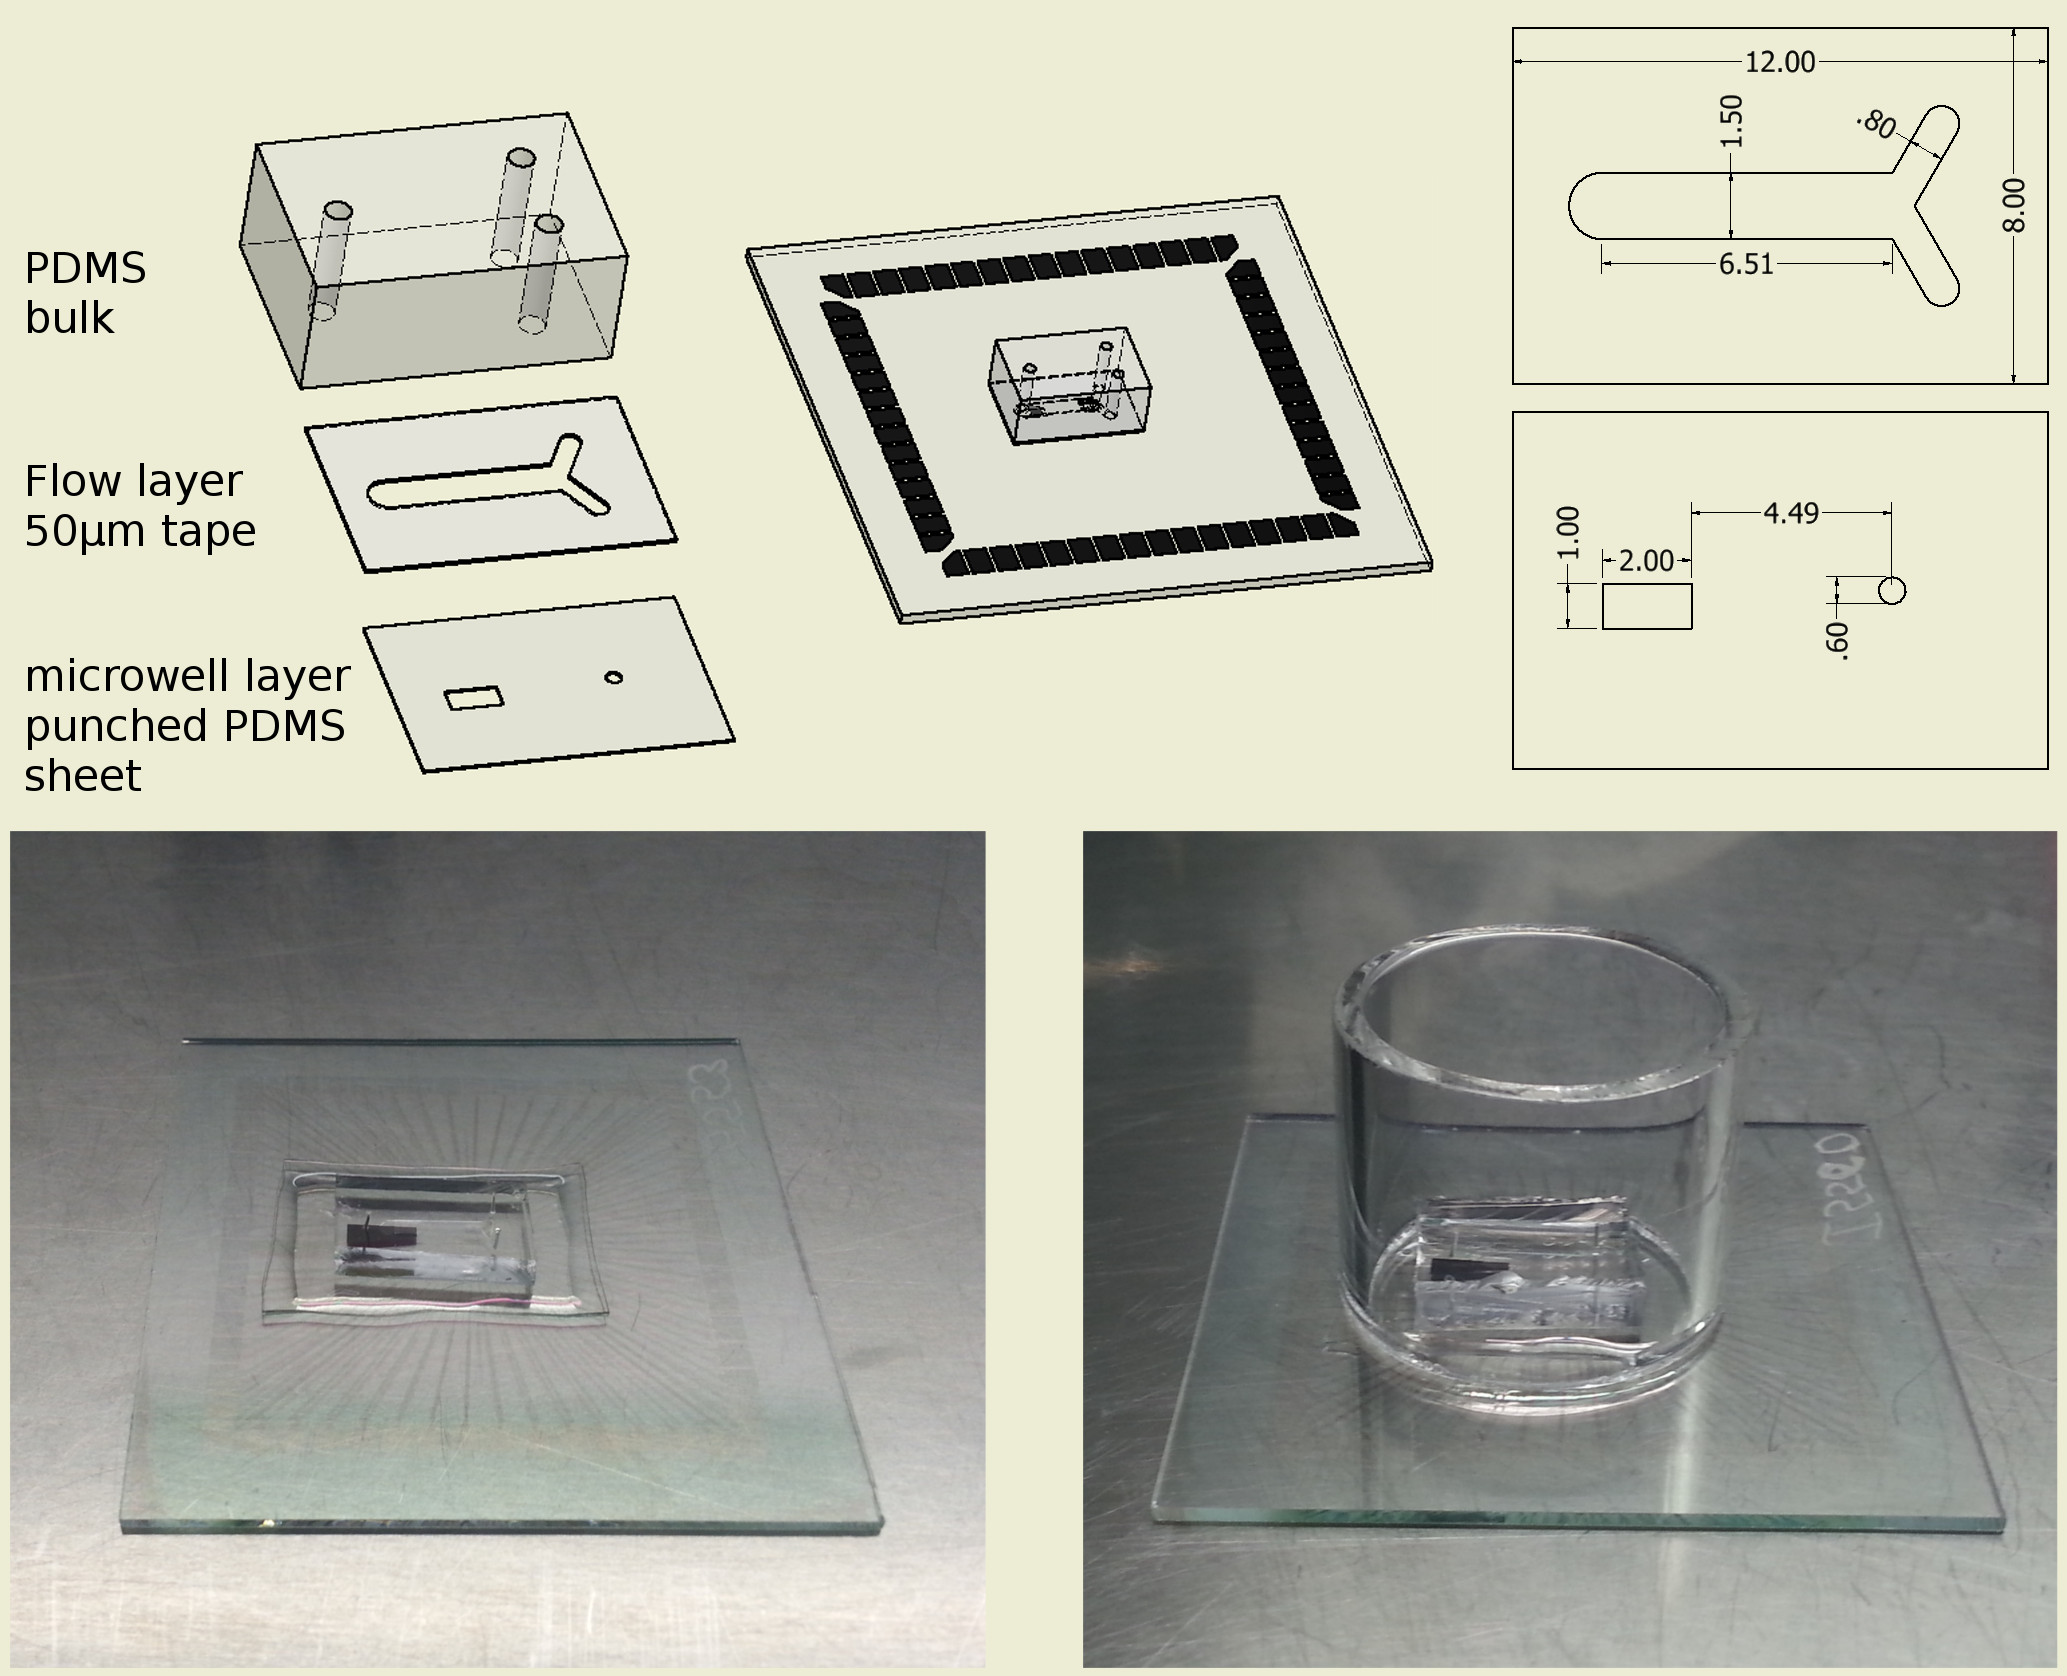
\includegraphics[width=15cm]{chapter6/figures/circularIllustration/circularIllustration.jpg}
       \caption[Illustration of the new microwell devices used for dopamine pulsing on a microculture]{\textbf{Illustration of the microwell devices.} Illustrations showing the constituent layers of the device laid out as well as assembled and joined to an MEA. The dimensions of the flow and microwell layers are also shown in millimeter units. Also shown are images of the device before and after gluing of glass cylinder to hold the media reservoir. Further details about the device fabrication are found in the text.}
       \label{fig:pulses:circularIllustration}

  \end{figure}

\subsection{PEI-then-all-tape devices}
    In preliminary versions of the device the microwell layer was composed of silicone transfer tape as this was expected to improve the bonding between the layers and reduce leaks. However, despite the good results obtained with devices made purely out of tape in section \ref{sec:devices:bonding}, the microcultures in this case exhibited poor adhesion and did not develop normally (figure \ref{fig:pulses:tapeMicroculture}). In a previous study toxic effects of leaching from PDMS, which is generally considered safe, presented themselves in microfluidic devices of extremely small geometries \cite{millet2007microfluidic}, presumably because of an increased leaching surface to media volume ratio. We reasoned that a similar issue arises in our devices but with tape being the source of the leaching so we switched to extracted PDMS (section \ref{sec:methods:fabrication}) for production of the microwell layer. Indeed this modification succeeded in providing the right conditions for microculture growth, as shown next.

  \begin{figure}[h]
       \centering
       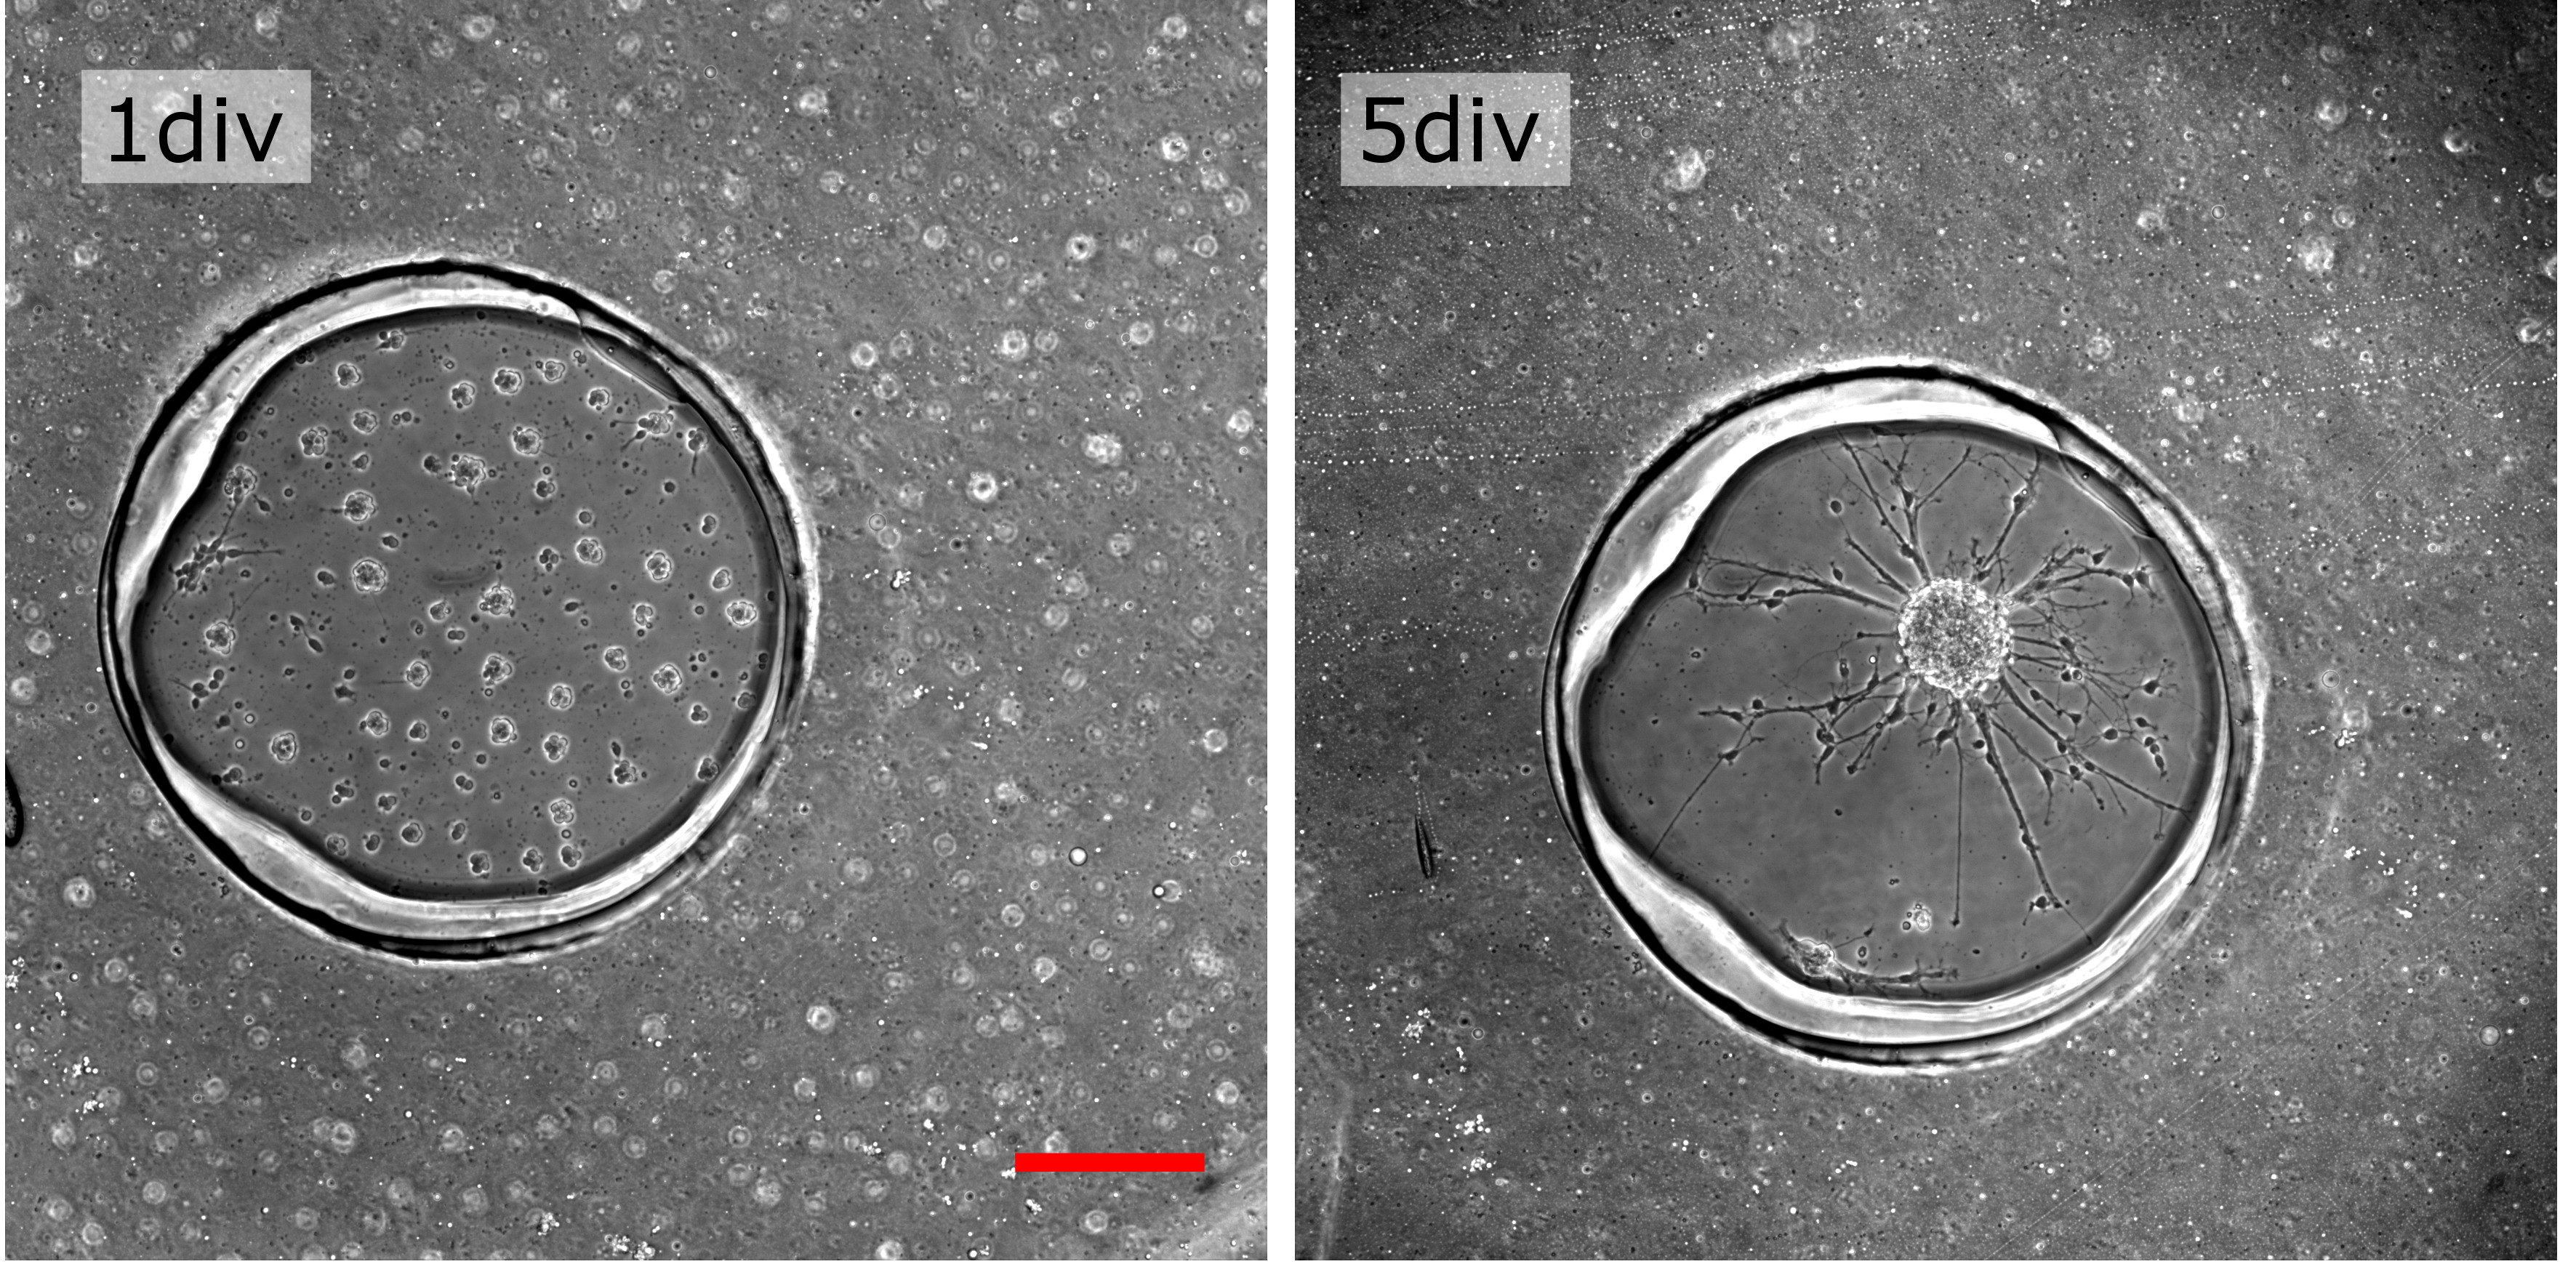
\includegraphics[width=15cm]{chapter6/figures/tapeMicroculture/tapeMicroculture.jpg}
       \caption[Microcultures grown in all-tape devices exhibit bad surface adhesion]{\textbf{Devices made purely out of silicone transfer tape are unsuitable for neuronal adhesion.} Images of a culture seeded into devices where both flow and microwell layers were made out of silicone transfer tape (\(50\) and \(125 \mu m\) thick, respectively). The cells aggregated immediately after plating and formed a single cluster after a few days. Scale bar is \(200 \mu m\) long and is consistent across both images.}
       \label{fig:pulses:tapeMicroculture}
  \end{figure}

    \subsection{PEI-then-PDMS-tape device}
    Microcultures generally grew well in the PDMS / tape chimera devices and were usually viable into the 4\textsuperscript{th} week \textit{in vitro} (figure \ref{fig:pulses:PDMSMicroculture}). However, and interesting side effect of the surface-then-bond (see sections \ref{sec:methods:bonding} and \ref{fig:devices:tapeCultures}) approach where the surface outside the microwell is not rendered cell adhesive was revealed: Older microcultures seemed to condense so that the microwell area occupied by the culture tissue became gradually smaller (figure \ref{fig:pulses:PDMSMicroculture} 19div). This shows that the process of generation of the culture tissue involves buildup of internal tension which is normally balanced by the the adhesion forces. In the case of the microcultures the limited availability of adhesion surface did not afford enough support to keep the tissue from condensing. This effect was not observed for the microcultures produces with the bond-then-surface approach in section \ref{sec:devices:microcultures}. It is likely that those microcultures were able to extend outside the microwell area so the balance between tissue mass and adhesion was more favorable for the latter.

    \begin{figure}[h]
       \centering
       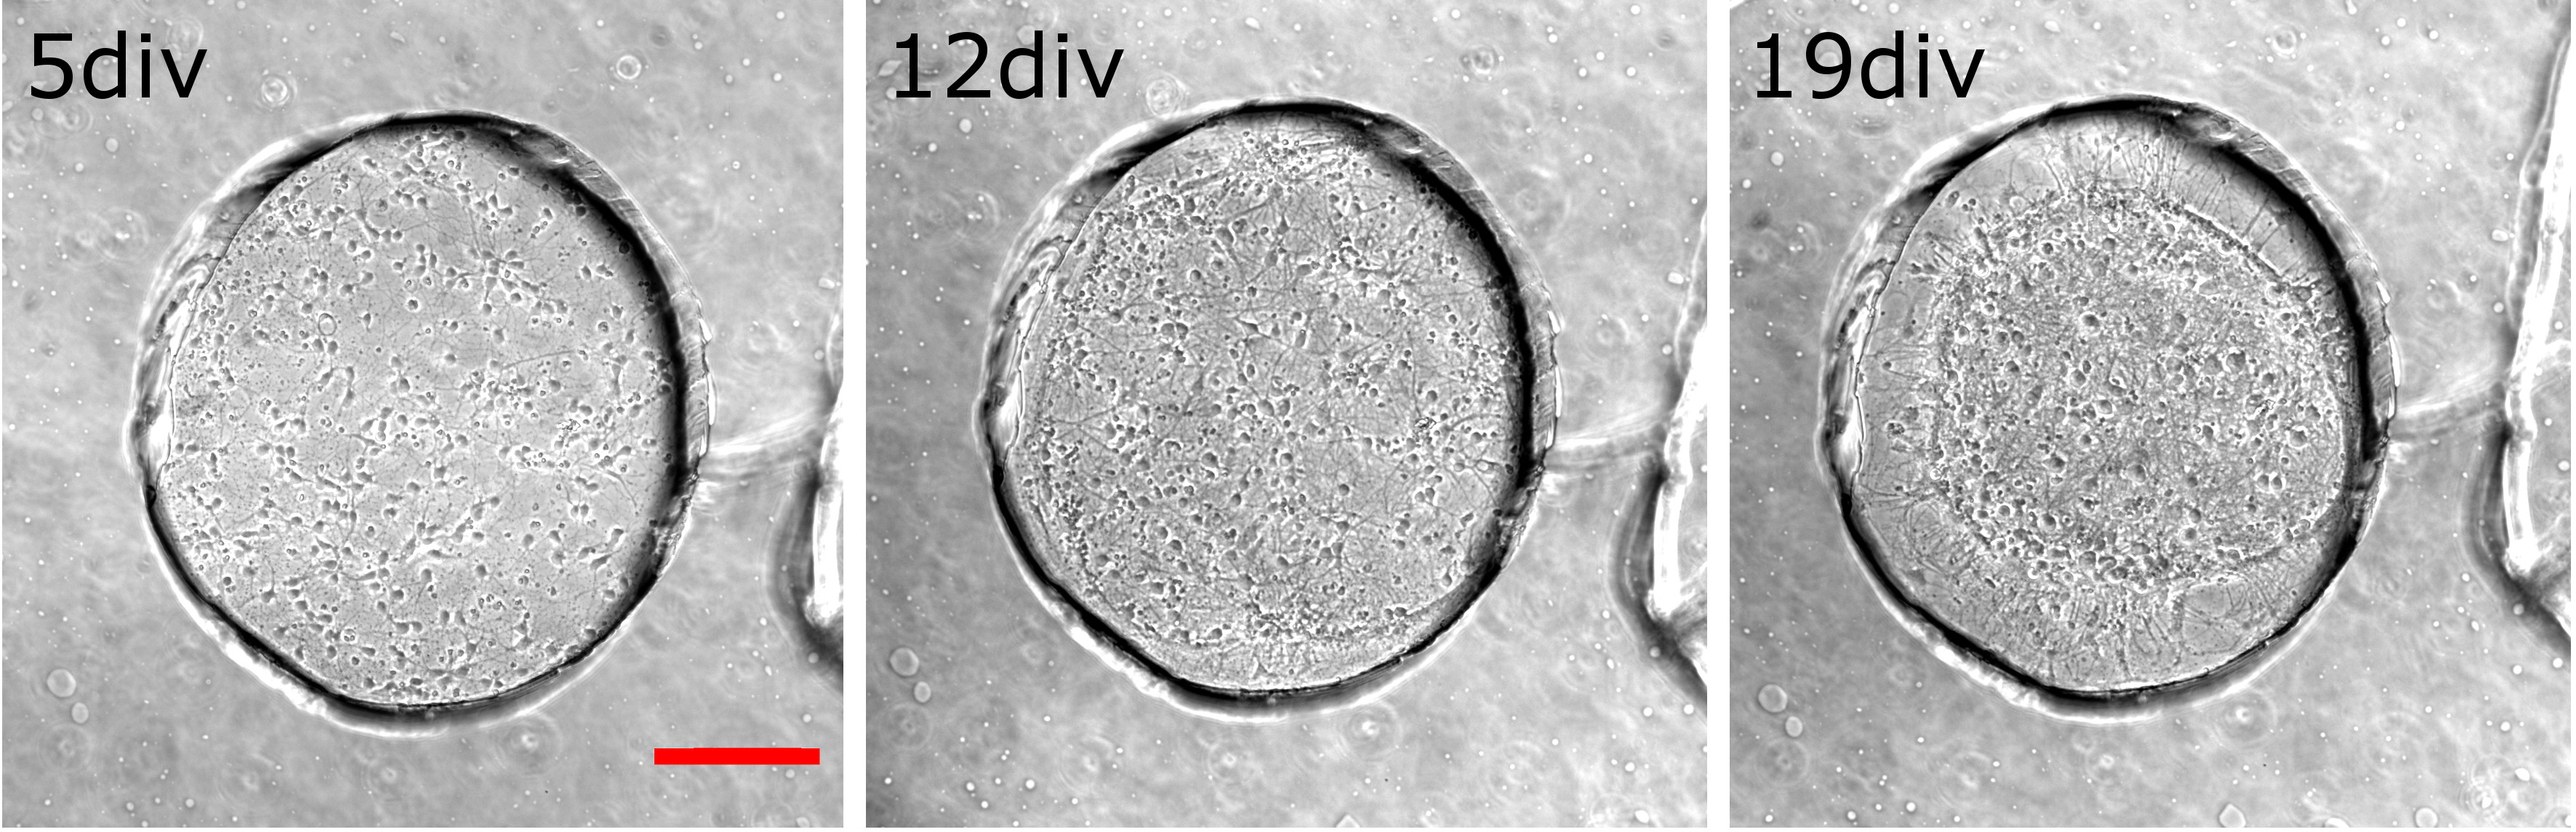
\includegraphics[width=15cm]{chapter6/figures/PDMSMicroculture/PDMSMicroculture.jpg}
        \caption[Development of microcultures is hybrid PDMS-tape devices]{\textbf{Devices with a PDMS microwell layer are conducive to good neuronal adhesion and development.} Images of a culture seeded into devices where the flow layer was made out of \(50\mu m\) tape and the microwell layer was made out of a \(120 \mu m\) thick PDMS sheet. The cells adhered well and developed similarly to standard cultures. After about 3 weeks the tissue began collapsing inwards. Scale bar is \(200 \mu m\) long and is consistent across all images.}
       \label{fig:pulses:PDMSMicroculture}
   \end{figure}

   We performed immunohistochemical staining on the cultures to make sure they develop normally and to receive further information on their cellular composition. We used antibodies for specific neuronal and glial structural proteins (\textbeta -tubulin and GFAP, respectively) as well as nuclear staining (DAPI) to visualize the location of the cell somas (Figure \ref{fig:pulses:PDMSMicrocultureStaining}). Interestingly, the neurites seem to be extremely tightly packed, to the level that they form a seemingly solid tissue. This might be a consequence of their confinement to the small area of the microwell and would explain why internal tissue tensions would exceed those of surface adhesion, driving the tissue to collapse on itself. Additionally, the cultures comprise a dense population of astrocytes. In recent years, it is becoming progressively accepted that astrocytes are an integral part of the synaptic structure and that they participate in the synaptic signalling \cite{araque1999tripartite}. Thus, astrocytes are necessary for neural function and their presence holds a promise that the microcultures, despite their unorthodox size, indeed may represent a functional cortical circuit.

   \begin{figure}[!htb]
       \centering
       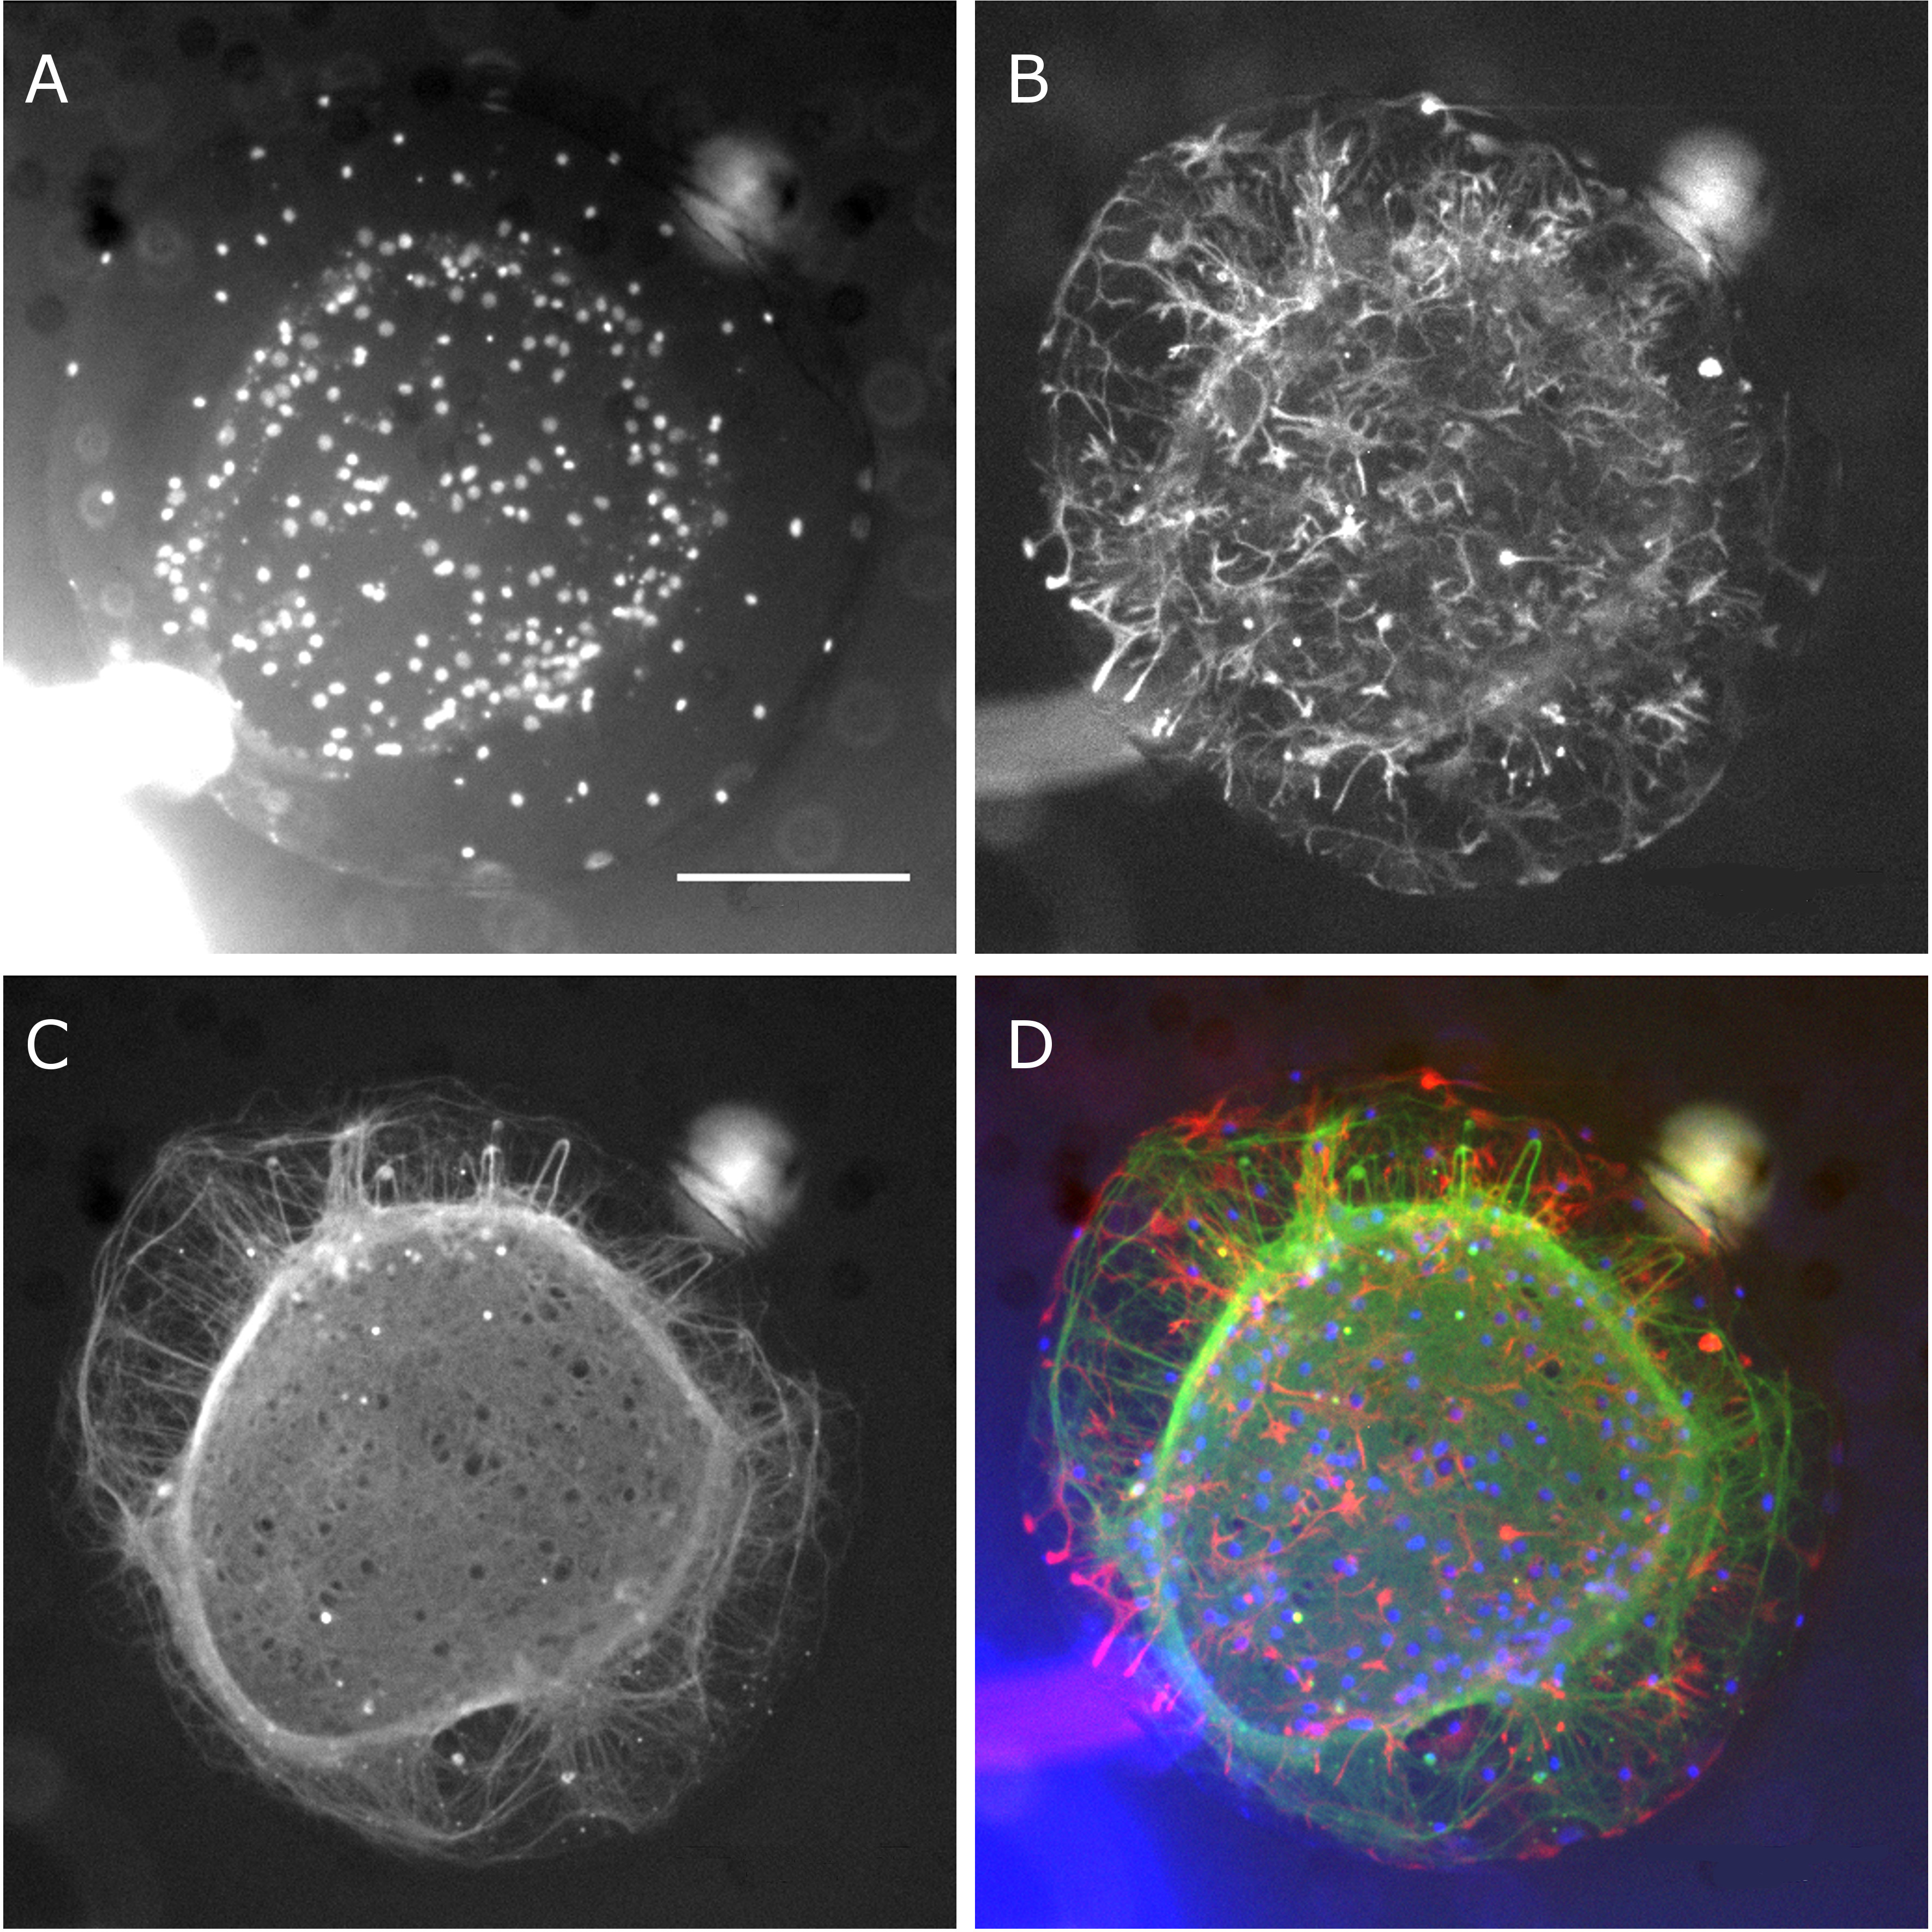
\includegraphics[width=15cm]{chapter6/figures/PDMSMicrocultureStaining/PDMSMicrocultureStaining.jpg}
       \caption[Immunohistochemistry of microcultures in hybrid PDMS-tape devices]{\textbf{Immunostaining of the microcultures indicates the presence of intact neuronal and astrocytic structural elements.} Images of immunohistochemical staining of the same culture shown in figure \ref{fig:pulses:PDMSMicroculture} at 23 days \textit{in vitro}. Staining agents are (A) DAPI, (B) anti-GFAP and (C) anti-\textbeta-tubulin. (D) Overlay of above staining images with pseudo colors. Staining shows a dense atrocytic presence and an intact neuritic network. Scale bar is \(200 \mu m\) long and is consistent across all images.}
       \label{fig:pulses:PDMSMicrocultureStaining}
    \end{figure}

    In section \ref{sec:devices:microcultures} we mentioned that the microwell devices that were based on the bond-then-surface paradigm were ineffective at keeping the microcultures confined to microwell area as neurites grew out onto the PDMS surface. In the case of the device of concern here, in virtue of the surface-then-bond approach where the areas outside the microwells were not cell adhesive, the microcultures did not grow out of the microwells and remained well restricted for over 3 weeks \textit{in vitro}. This is shown in figure \ref{fig:pulses:clearanceDemonstration} which shows the PDMS sheet around a microwell at days 1 and 19 \textit{in vitro}. The PDMS sheet remained clear of neurites throughout the development period. Some seeded cells were not cleared by the flushing but these remained completely latent and no observable connections with the main microculture were observed.

    \begin{figure}[!htb]
       \centering
       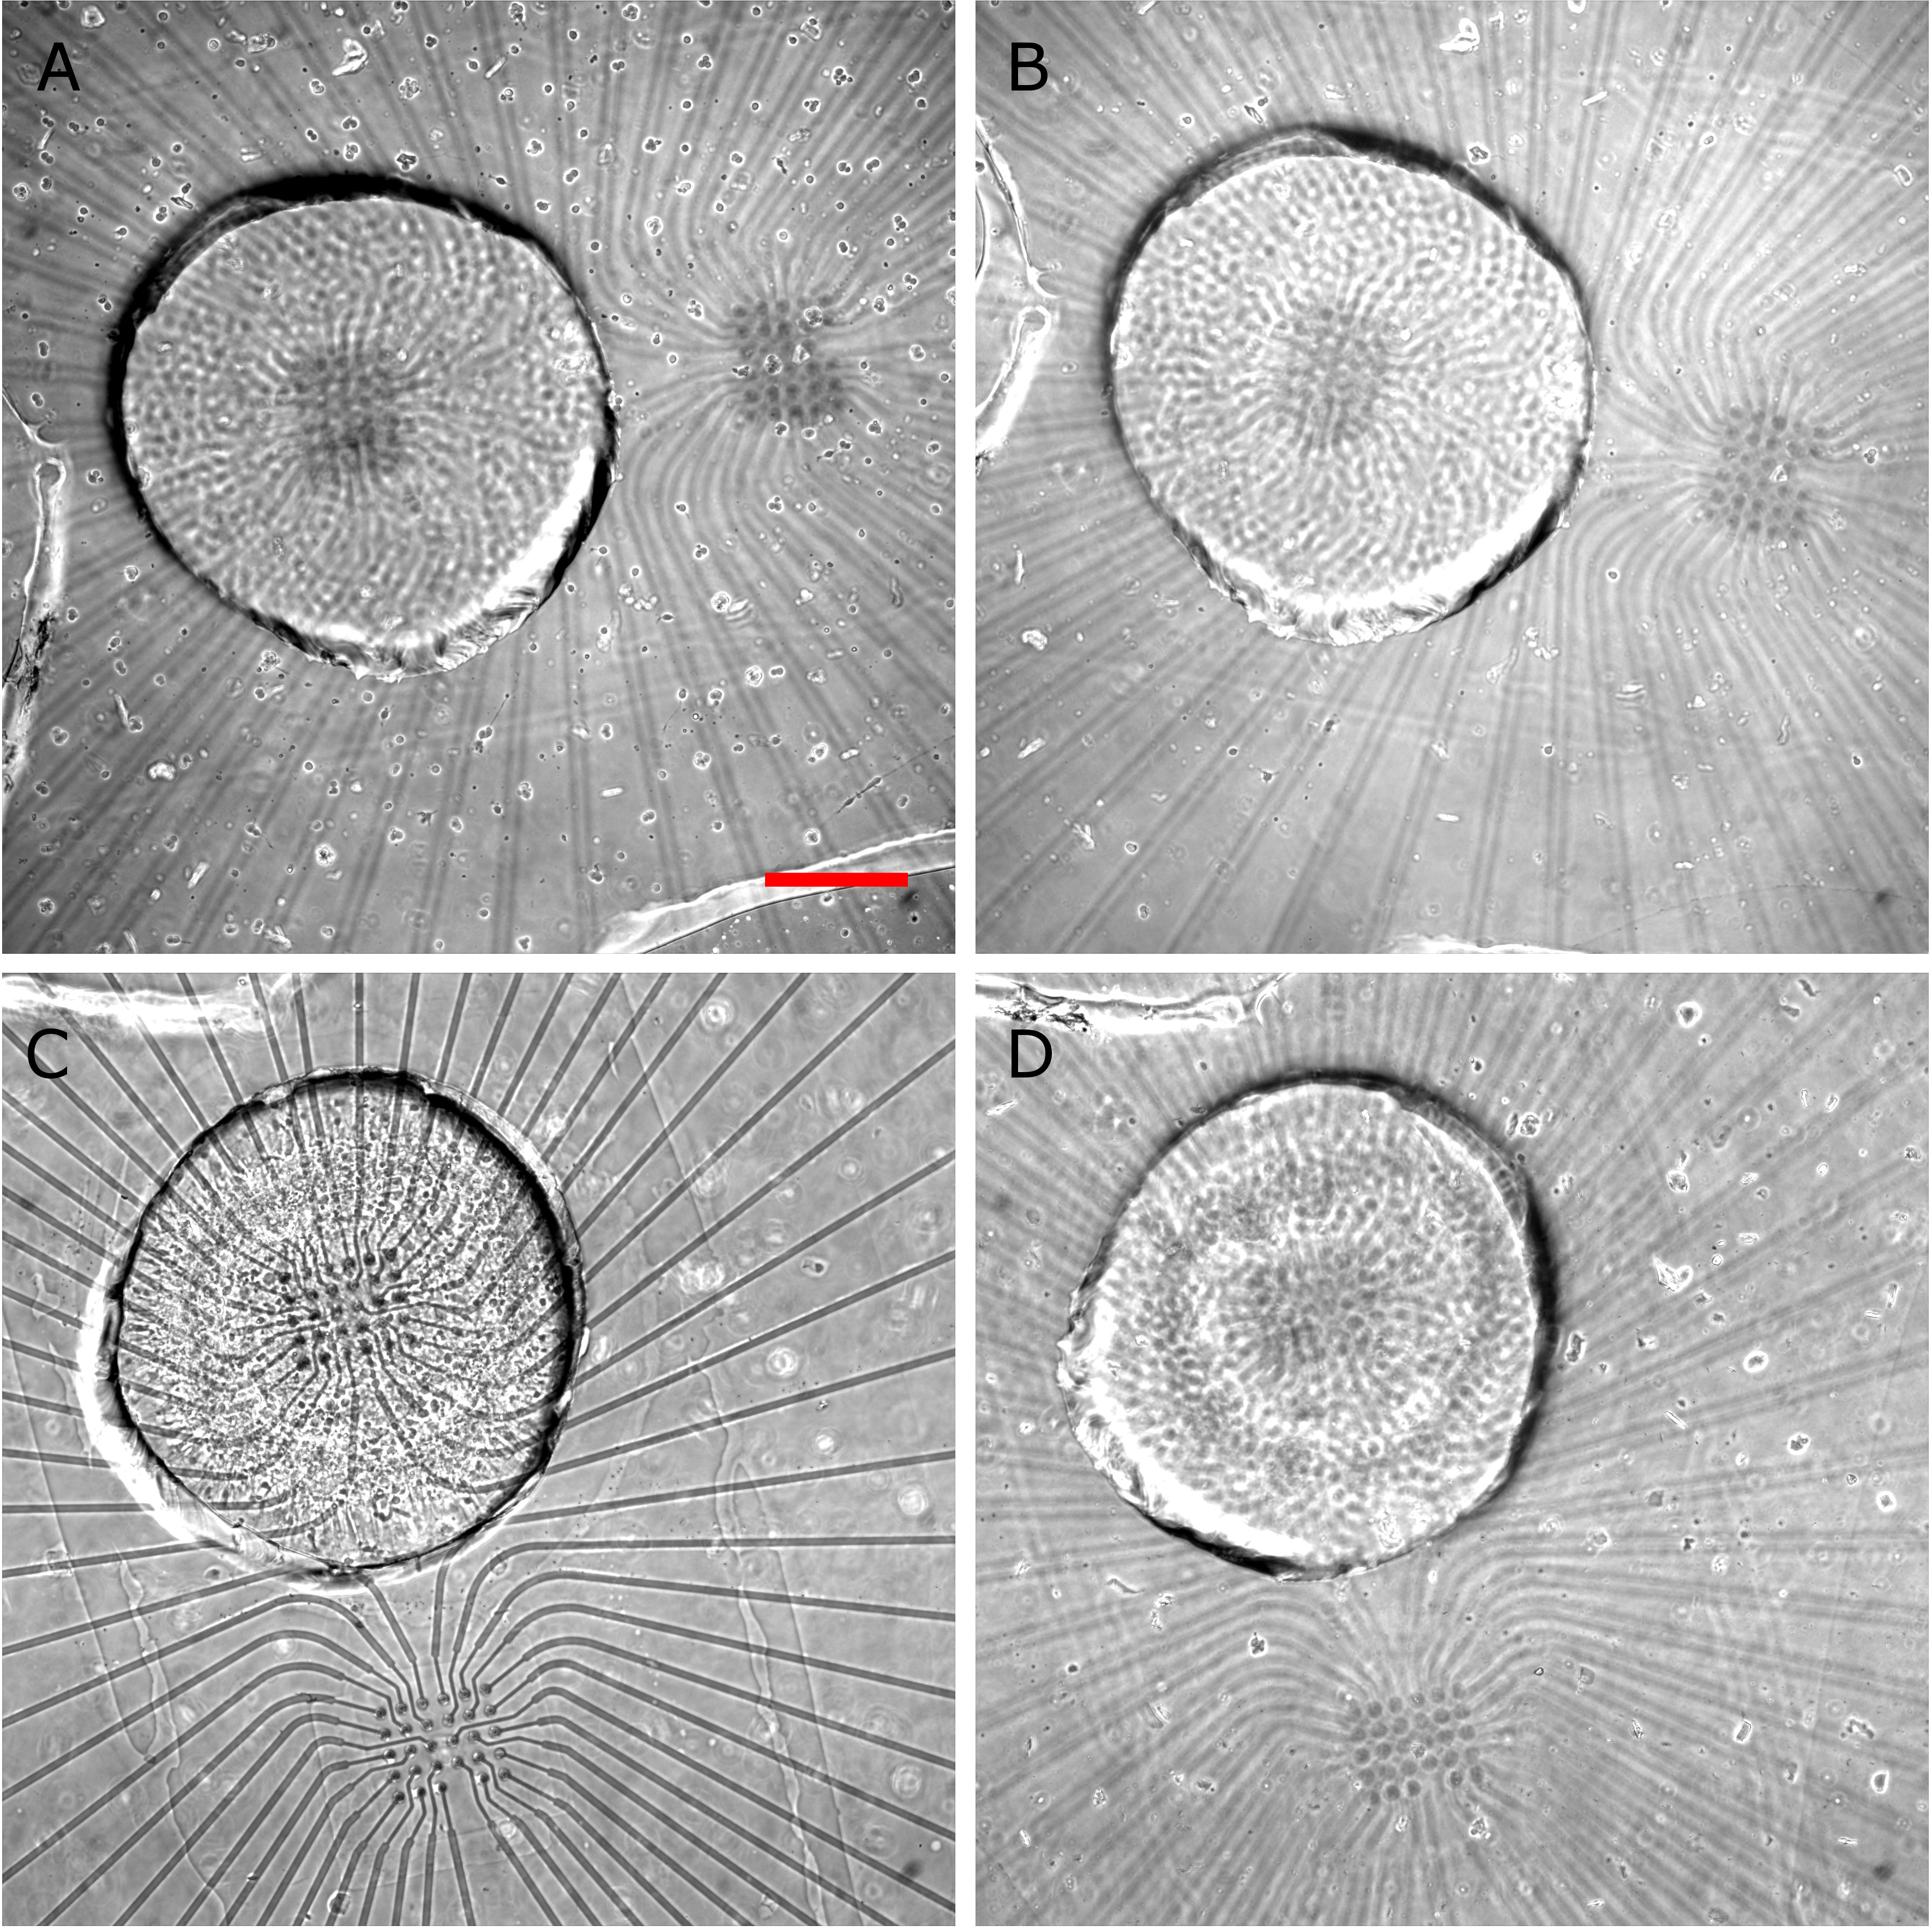
\includegraphics[width=15cm]{chapter6/figures/clearanceDemonstration/clearanceDemonstration.jpg}
       \caption[Effectiveness of surface-then-bond in maintaining an isolated microculture]{\textbf{No neuritic growth into the top of the PDMS sheet is seen even after 3 weeks \textit{in vitro}.} Images of a seeded microculture and the surrounding top surface as follows: (A) Top surface after 1 day \textit{in vitro} before flushing. (B) Same as A following removal of excess cells via flushing. (C) Microculture at 19 days \textit{in vitro} (top surface is out of focus). (D) Top surface of C. Scale bar is \(200 \mu m\) in is consistent across all images.}
       \label{fig:pulses:clearanceDemonstration}
   \end{figure}

   The microculture confinement is further demonstrated in figure \ref{fig:pulses:topOfSheetTaining} which shows immunohistochemical staining of the same culture as in figure \ref{fig:pulses:PDMSMicrocultureStaining} (at 23 days \textit{in vitro}) but focusing on the top surface of the PDMS sheet. The nuclear staining clearly shows that cell somata are present outside the microwell area this stage. However, these somata are strictly co-localized with astrocytic (GFAP) staining whereas neuronal staining (\textbeta -tubulin) is completely absent from the top surface. This example serves to demonstrate that by 3 weeks \textit{in vitro} some astrocytes have migrated outside the microwell onto the surrounding PDMS. Nevertheless, even though one may suspect that these renegade astrocytes could serve as a substrate for subsequent neuronal migration, such a process has yet to occur at this point.

   \begin{figure}[!htb]
       \centering
       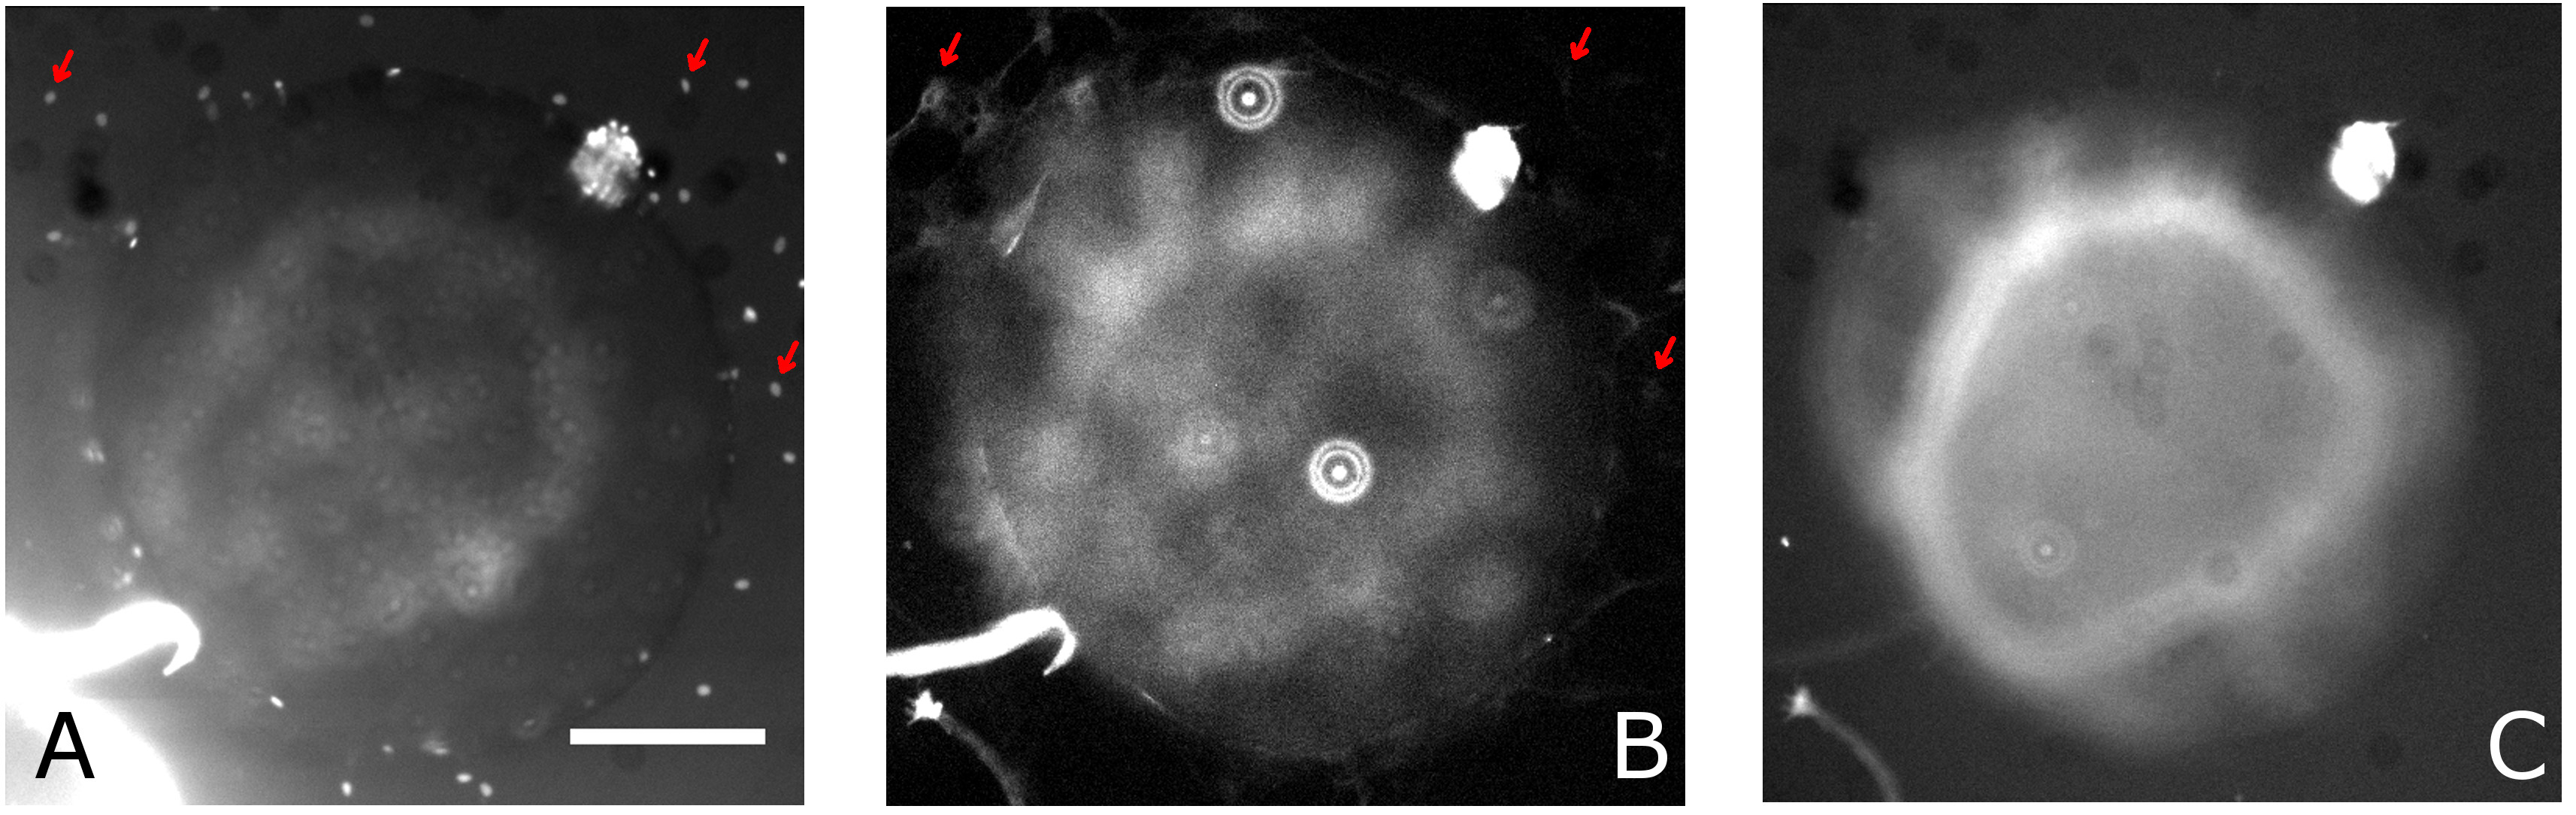
\includegraphics[width=15cm]{chapter6/figures/topOfSheetSTaining/topOfSheetStaining.jpg}
        \caption[Effectiveness of surface-then-bond in maintaining an isolated microculture - immunostaining evidence]{\textbf{No neurite growth into the top of the PDMS sheet is seen even after 3 weeks \textit{in vitro}.} Immunostaining images of the same culture as in figure \ref{fig:pulses:PDMSMicrocultureStaining} focusing on the top surface. Staining agents are: (A) DAPI, (B) anti-GFAP and (C) anti-\textbeta-tubulin. Although some cells are present on the top surface they are co-localized with astrocytic staining (examples are indicated by red arrows) whereas neuronal staining is completely absent. Scale bar is \(200 \mu m\) and is consistent across all images.}
       \label{fig:pulses:topOfSheetTaining}
   \end{figure}

   \subsection{Network activity in microcultures}
   We performed a pilot study where we monitored the spontaneous as well as evoked activity of the microcultures at two different plating densities. The selection of the plating density was based on the earlier microculture viability study (section \ref{sec:devices:microcultures}) where it was established that a minimum area density of \(1500 cells\cdot mm^{-2}\) is required for the microcultures to develop properly (i.e., not exhibit an increased degeneration rate as compared to standard cultures). Since the microcultures used here are bigger than the ones in the earlier study we decided to attempt using a lower density in hope that it would reduce the collapse of the tissue described above but still sustain the viability. Thus the plating densities we explored were either \(6\times 10^{6}\) or \(12\times 10^{6} cells\cdot ml^{-1}\). (corresponds to area densities of \(\approx 1000\) or \(2000 cells\cdot mm^{-2}\) and termed `single density' or `double density', respectively). In the case of the single density microcultures, we found it hard to generate consistent evoked responses by means of electrical stimulations (i.e., most of the electrodes either did not generate responses at all or induced weak and inconsistent ones) which might indicate that the synaptic communication was not fully formed. Indeed immunohistochemical staining performed on these microcultures showed that in many of them the neuronal tissue was heavily fragmented and there was no appreciable astrocytic staining.

   Strong differences between single density and double density microcultures were also presented when the cultures were placed under flow. The flow sessions were performed on old microcultures at ages 18-22 days \textit{in vitro} and consisted of fast flow with self media as these conditions were shown to allow stable network activity (section \ref{sec:crossFlow:oldSelf}). The age range used here is slightly lower than in the original study because in some cases the tissue collapse dictated earlier experimentation. Out of 7 single density cultures subjected to flow only 2 maintained any form of stimulation response, in one of them, this response was abolished within 20 minutes. Out of 24 double density microcultures, 14 maintained a consistent stimulation response for an extended period of time (hours). The final protocol therefore used the double density parameter. It should be noted that the inconsistency exhibited by the microcultures is quite different from how the standard cultures in chapter \ref{chap:activityAndFlow} responded to flow. In that case, all old cultures maintained functionality under flow with self media, without exception. In section \ref{sec:crossFlow:interp} we hypothesized that the performance of a culture under flow is determined by how well the chemistry of the flow media is `matched' with the local chemical microenvironment around the culture which, in turn, depends on its developmental stage. An explanation for the inconsistency might therefore be that the microcultures, with their unorthodox size, have a different developmental time course and so the self media, which reflects the developmental stage of the external support culture, is more likely to be unmatched. Nevertheless, the 60\% success rate was found to be adequate and so we proceeded with the above-mentioned flow protocol.

   The microcultures generally exhibited synchronized bursting dynamics similar to the standard (macro) cultures at the same age group. This was manifested in a similar level of synchronization and burst rate (figure \ref{fig:pulses:microcultureStimControl} A, unbalanced t-test, \(p=0.28\) and \(0.11\), respectively). However, the level of activity in the microcultures was significantly lower (unbalanced t-test, \(p=0.033\)). It is important to note, though, that the distribution of activity levels was not trivial. Out of 5 monitored microcultures, 2 exhibited activity levels within the literature range (\(0.7\) and \(1 Hz\), literature range is \(0.4-1.5Hz\), see section \ref{fig:activity:mouseRatComparison}) whereas 3 were almost completely silent (\(0.1\), \(0.02\) and \(0.03Hz\)). The silent cultures still had bursts detected in them but these consisted of single or very few spikes on a small portion of the electrodes. Nevertheless, the low activity level did not mean that these microculture were not able to generate strong reverberative activity as, remarkably, when they were continuously stimulated with test pulses at \(0.2Hz\) the recorded activity levels went up to \(\approx 1Hz\) (figure \ref{fig:pulses:microcultureStimControl}) and the PSTHs were as intense as in the macrocultures (will be shown later in section \ref{sec:pulsing:dopamine}). Thus to summarize, provided that electrical stimulation is applied, the microcultures exhibit reverberative network activity and are therefore appropriate for use in the context of neuromodulator signalling and plasticity.


    \begin{figure}[h]
       \centering
       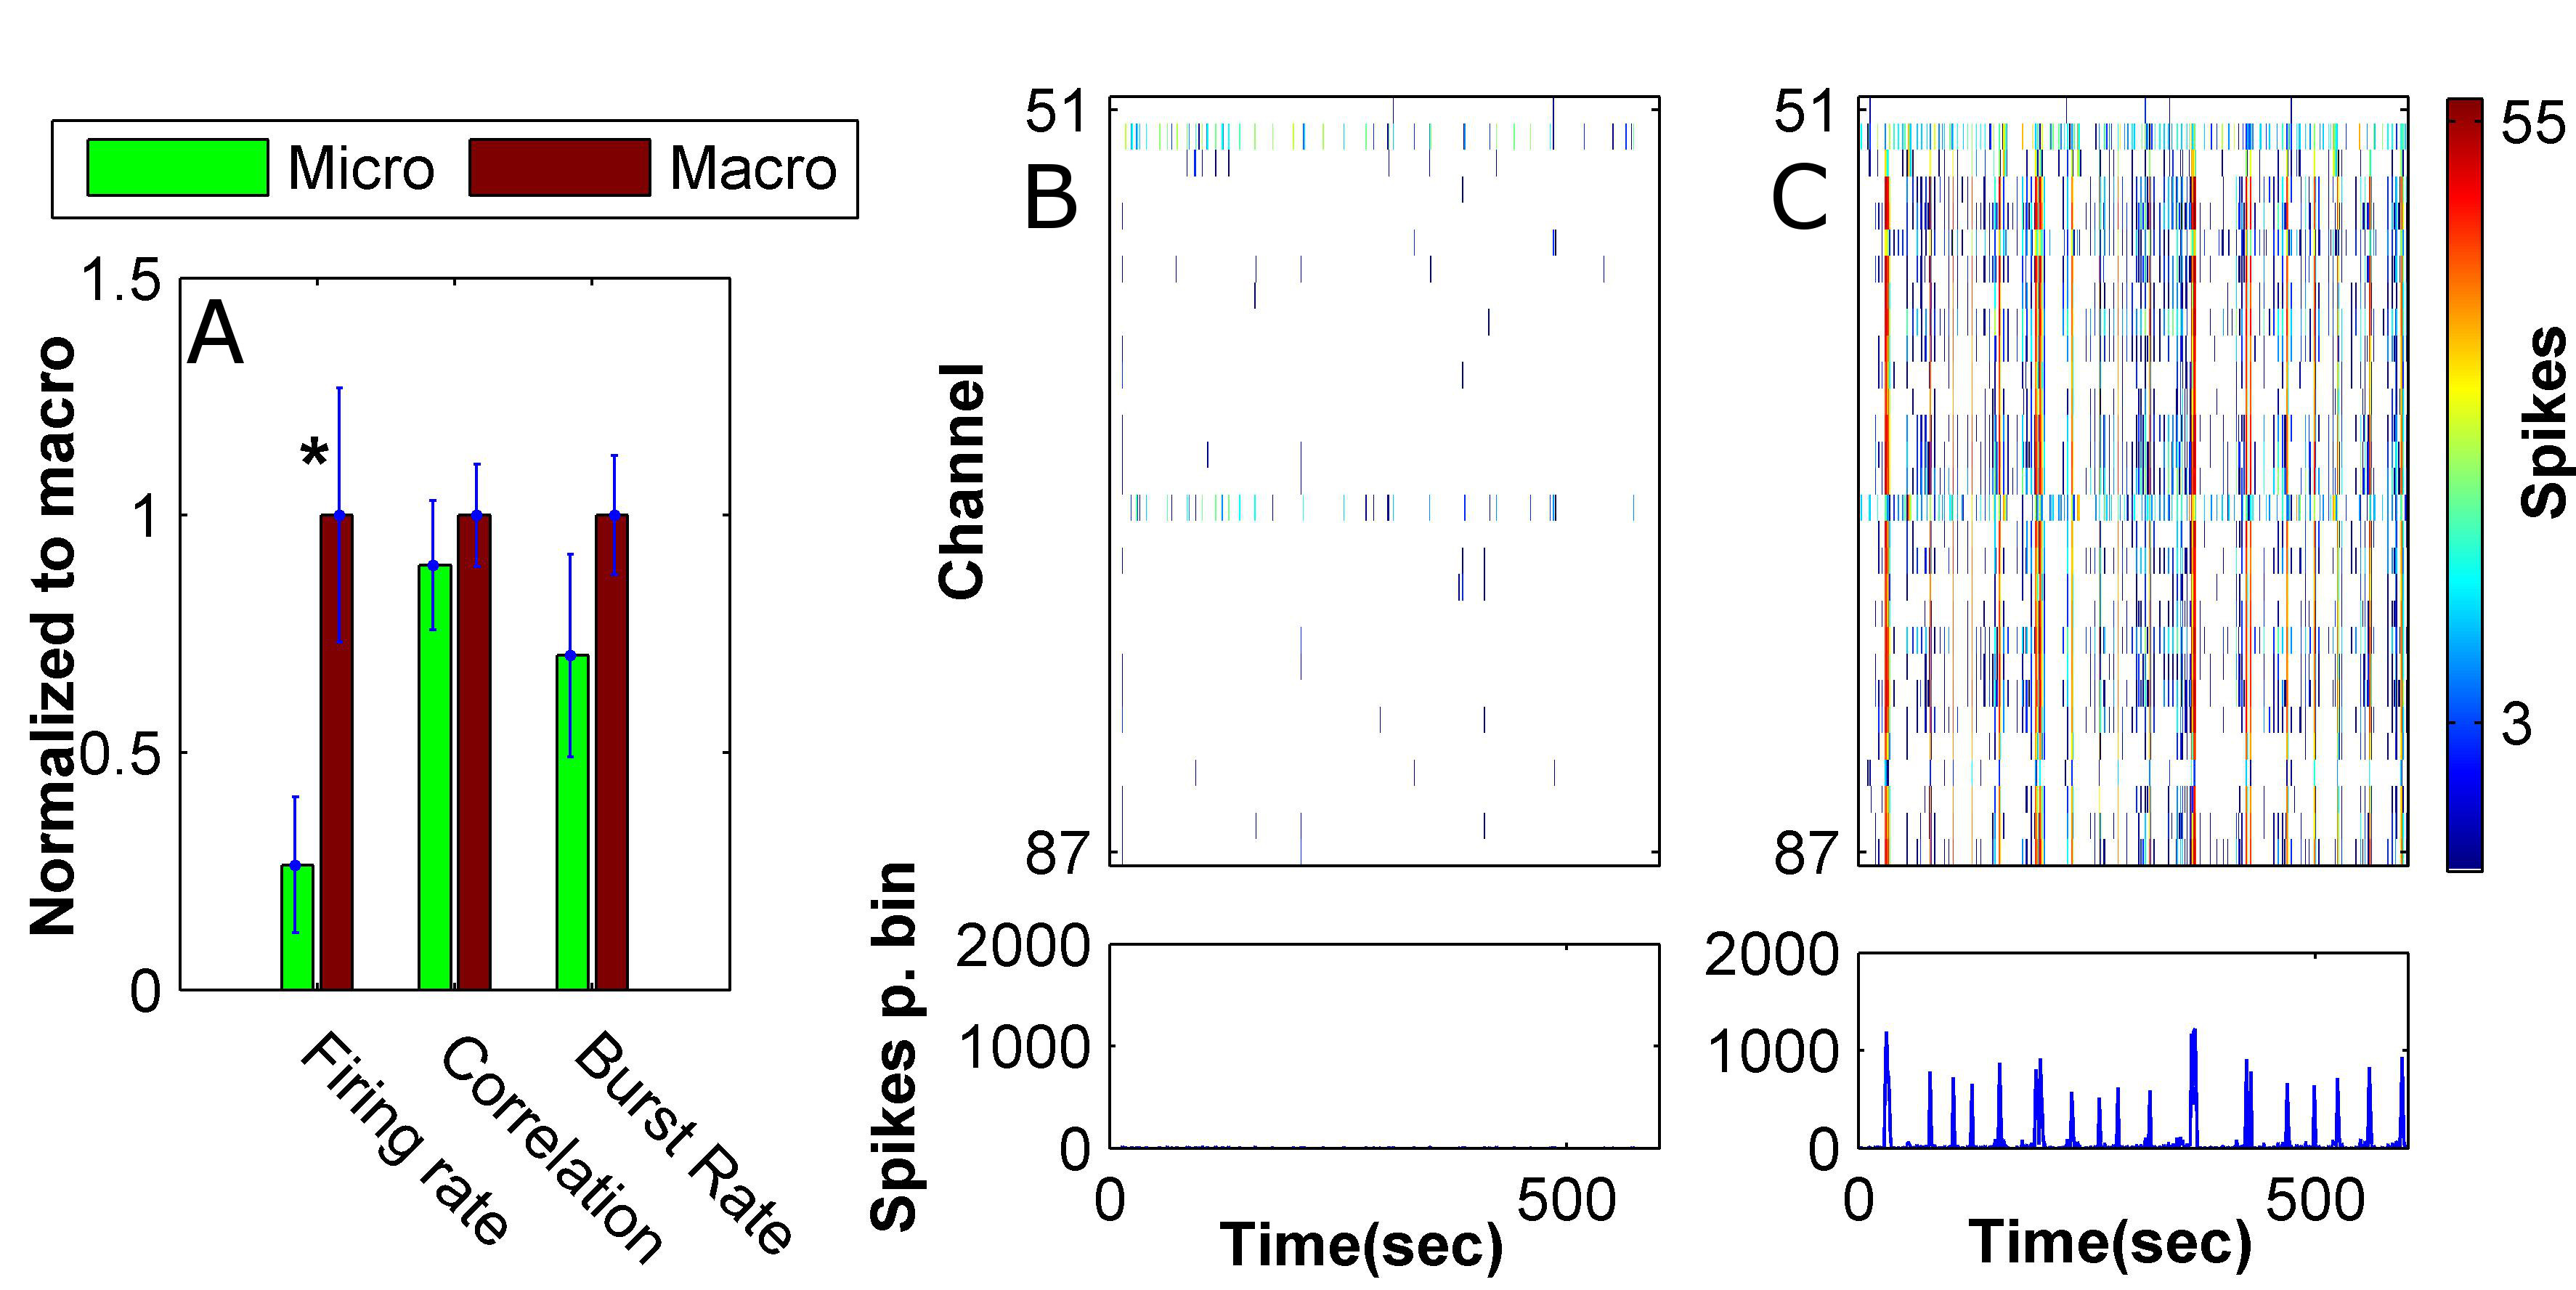
\includegraphics[width=15cm]{chapter6/figures/microcultureStimControl/microcultureStimControl.jpg}
       \caption[Spontaneous and evoked activity in microcultures]{\textbf{Microcultures show synchronized activity dynamics but sometimes require electrical stimulation to produce network wide events.} (A) Comparison of activity and bursting measures between macro- and micro-cultures. (B-C) Example raster plots of a microculture which exhibited low levels of spontaneous activity with and without electrical stimulation at \(0.2 Hz\), respectively. The shown time frame is too large to discern individual synchronized events and is shown to convey the dominance of the stimulations. Raster plots use bins of 1.2 seconds. Asterisk indicates a statistically significant difference between macro and microcultures at the given measure at a 95\% level of confidence. Data are based on n=5 and 8 double density microcultures and macrocultures from the same age group, respectively.}
       \label{fig:pulses:microcultureStimControl}
   \end{figure}

\section{Pulsing performance in microculture devices}
This section describes a visualization of the dynamics of agonist delivery within the microwell devices through imaging of the pulse action with a fluorescent tracer (fluorescein). It will also present data from an accompanying numerical simulation in Comsol. The reason for developing the numerical simulation is twofold: Firstly, the imaging, which is performed with dark field microscopy, is effective at discerning the agonist distribution in the plane parallel to the device axis. The Z axis distribution (i.e., the distribution along the height of the device), however, is not available and is recorded only as the sum of the fluorescence along that axis. Thus, to obtain an explicit account of the agonist concentration around the cells (i.e., bottom of the microwell), a 3D model is required. We therefore used the visualization to select the model parameters and as an experimental reference to make sure it generates a realistic output. The model was then used to extract the concentration at the cells. Secondly, once the model is shown to be realistic it can be used as a design tool for achieving specific pulsing patterns. We demonstrated how this may be used to achieve pulsing time scales that match phasic dopamine signalling in densely innervated brain areas.

  \subsection{Analysis of pulsing visualized by fluorescein}
  \label{sec:pusling:fluo}
  The visualization of the pulse dynamics was performed with the same imaging system as described in section \ref{sec:methods:flow} but with an \(4\times\) objective which allowed the entire channel width to fit within the field of view. In these experiments, DDW was used to for the blank (media without agonist) stream and 0.002\% (w/v) fluorescein was used for the agonist stream. This concentration of fluorescein was found to provide a linear relationship between the cross section depth and the intensity of the measured fluorescent signal (this was tested in the cross flow devices from chapter \ref{chap:activityAndFlow} where the layers are known to be of the same height). The pulse dynamics are controlled through switching between two flow modes: the `baseline' mode where the flow rates were set to \(100\) and \(5 nL\cdot s^{-1}\) for the blank and agonists channels, respectively, and a `pulse' mode where these rates were flipped. When these modes are continuously set the microwell is completely contained within the respective stream. The pulse action was generated by transiently switching to the pulse mode for 1.5 seconds and then reverting back to baseline. This period was found sufficient for the agonist stream to shift just enough to cover the entire microwell area before shifting back. An example of such a fluorescein-visualized pulse sequence is shown in figure \ref{fig:pulses:pulseSequence}.

  \begin{figure}[h]
       \centering
       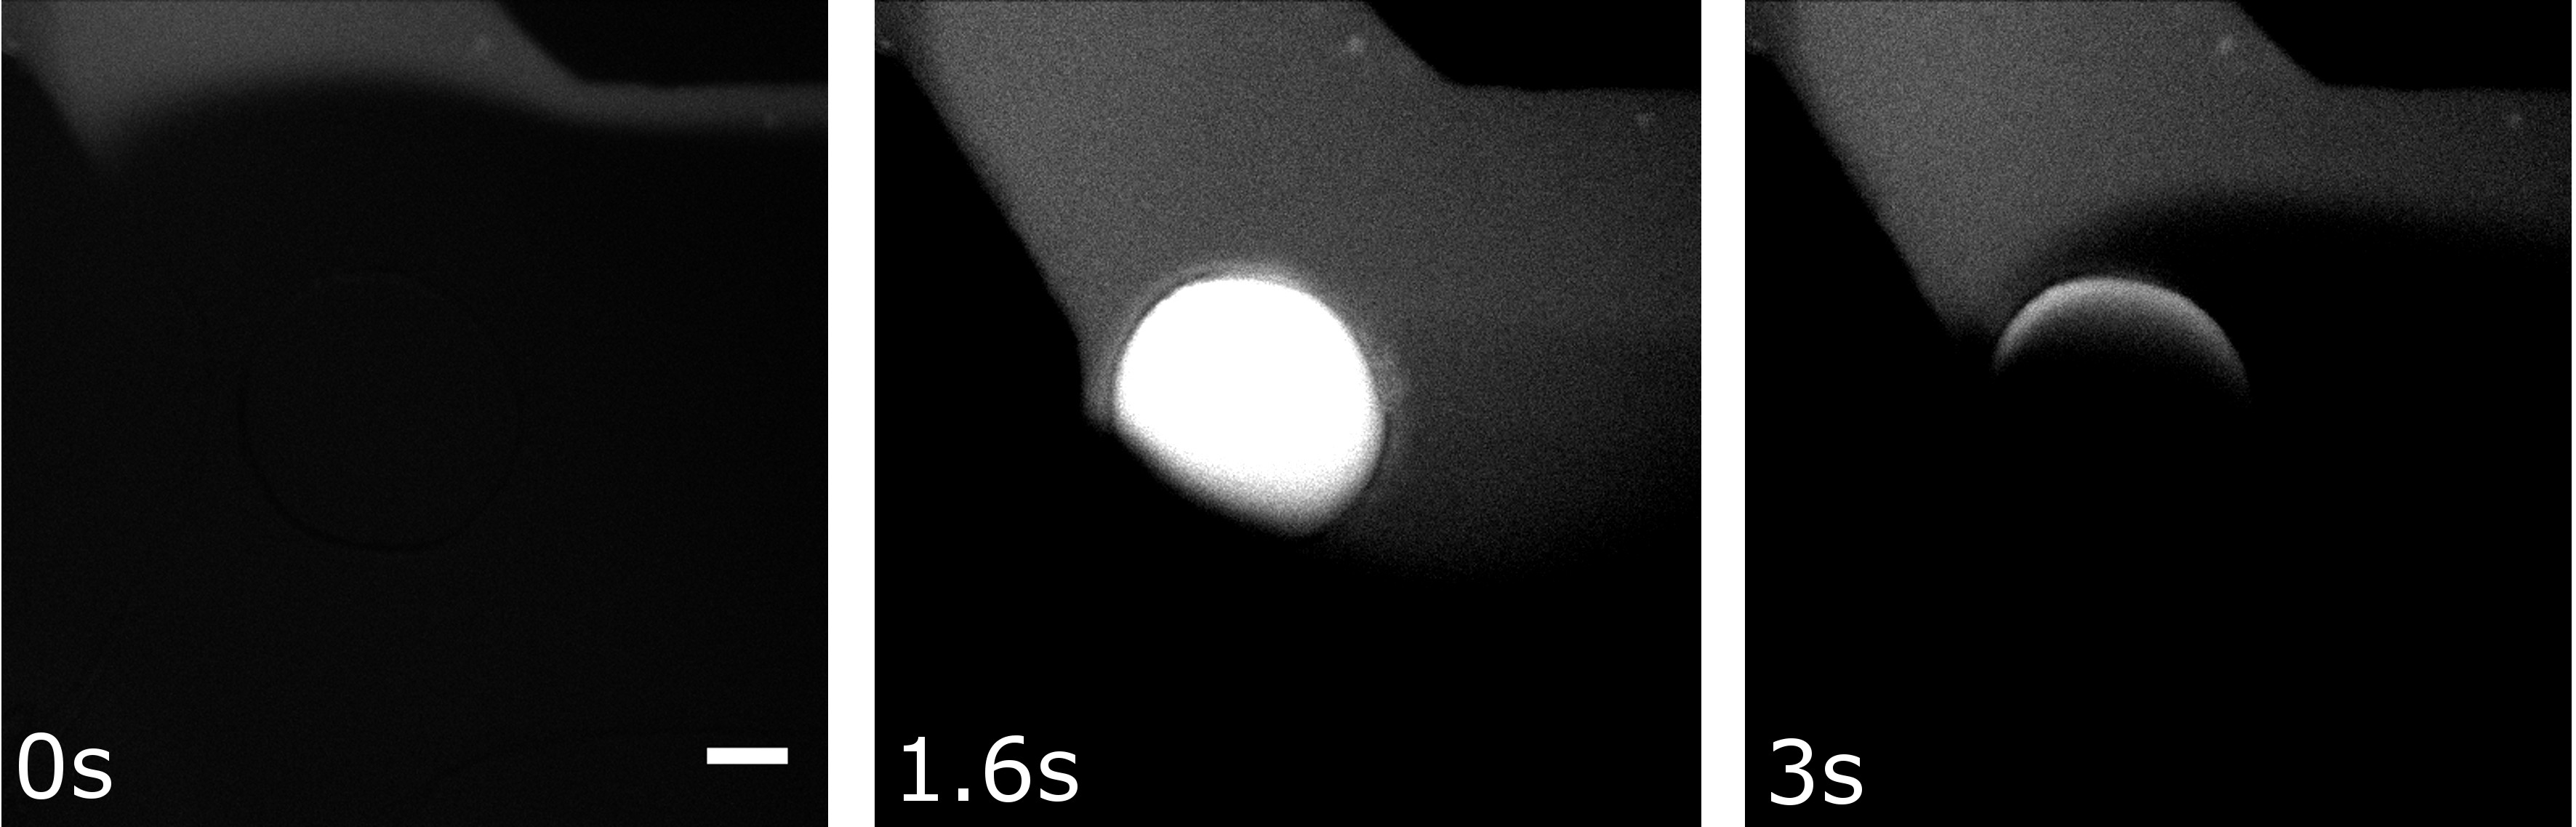
\includegraphics[width=15cm]{chapter6/figures/pulseSequence/pulseSequence.jpg}
       \caption[Fluorescence visualization of agonist pulsing]{\textbf{The time scales of the concentration transient are interrogated using fluorescein in the agonist stream.} Scale bar is \(200\mu m\) long and is consistent across all images.}
       \label{fig:pulses:pulseSequence}
  \end{figure}

  We now describe the full procedure used to obtain quantitative temporal data from the fluorescein measurements. A pulsing visualization session was initiated by setting the system to pulse mode for 120 seconds. This assured that the microwell would completely fill up with agonist and provided a reference value for microwell saturation. This was followed by 120 seconds of baseline to make sure that the microwell was completely cleared of the fluorescent tracer. Finally, 10 pulses (i.e., switching to pulse mode for 1.5 seconds and then back to baseline) were applied at 20 second intervals. The analysis of the data commenced by defining ROIs where it is desirable to know the concentration time course and extracting fluorescence traces (averaged over the ROIs). For each of the ROIs a square pulse was fitted to the initial segment of the fluorescent trace during which the microwell was entirely inside the agonist stream to obtain a saturation (reference) value. The pulse waveforms where then collected, averaged and normalized to this value. The resultant signal represents the time course of  ROI saturation during a pulse (i.e., the proportion of the device volume inside the ROI occupied by agonist). This analysis pipeline is illustrated by figure \ref{fig:pulses:fluoAnalysis} for two large ROIs, one encompassing the microwell and the second outside of it. Figure \ref{fig:pulses:fluoAnalysis} D shows the the microwell ROI saturation signal reaches a lower value and persists longer than the outside ROI even though the latter is positioned further along the flow line. This reflects the extra time required for the microwell to become filled up and then depleted of agonist. The normalization method described here allows to directly compare the experimentally derived concentration pulse time course to the one generated by the model and also allowed averaging experiments performed on different devices in different lighting and optical conditions. Such ROI saturation time courses will be compared to numerical simulations in the next section.

  \begin{figure}[!htb]
       \centering
       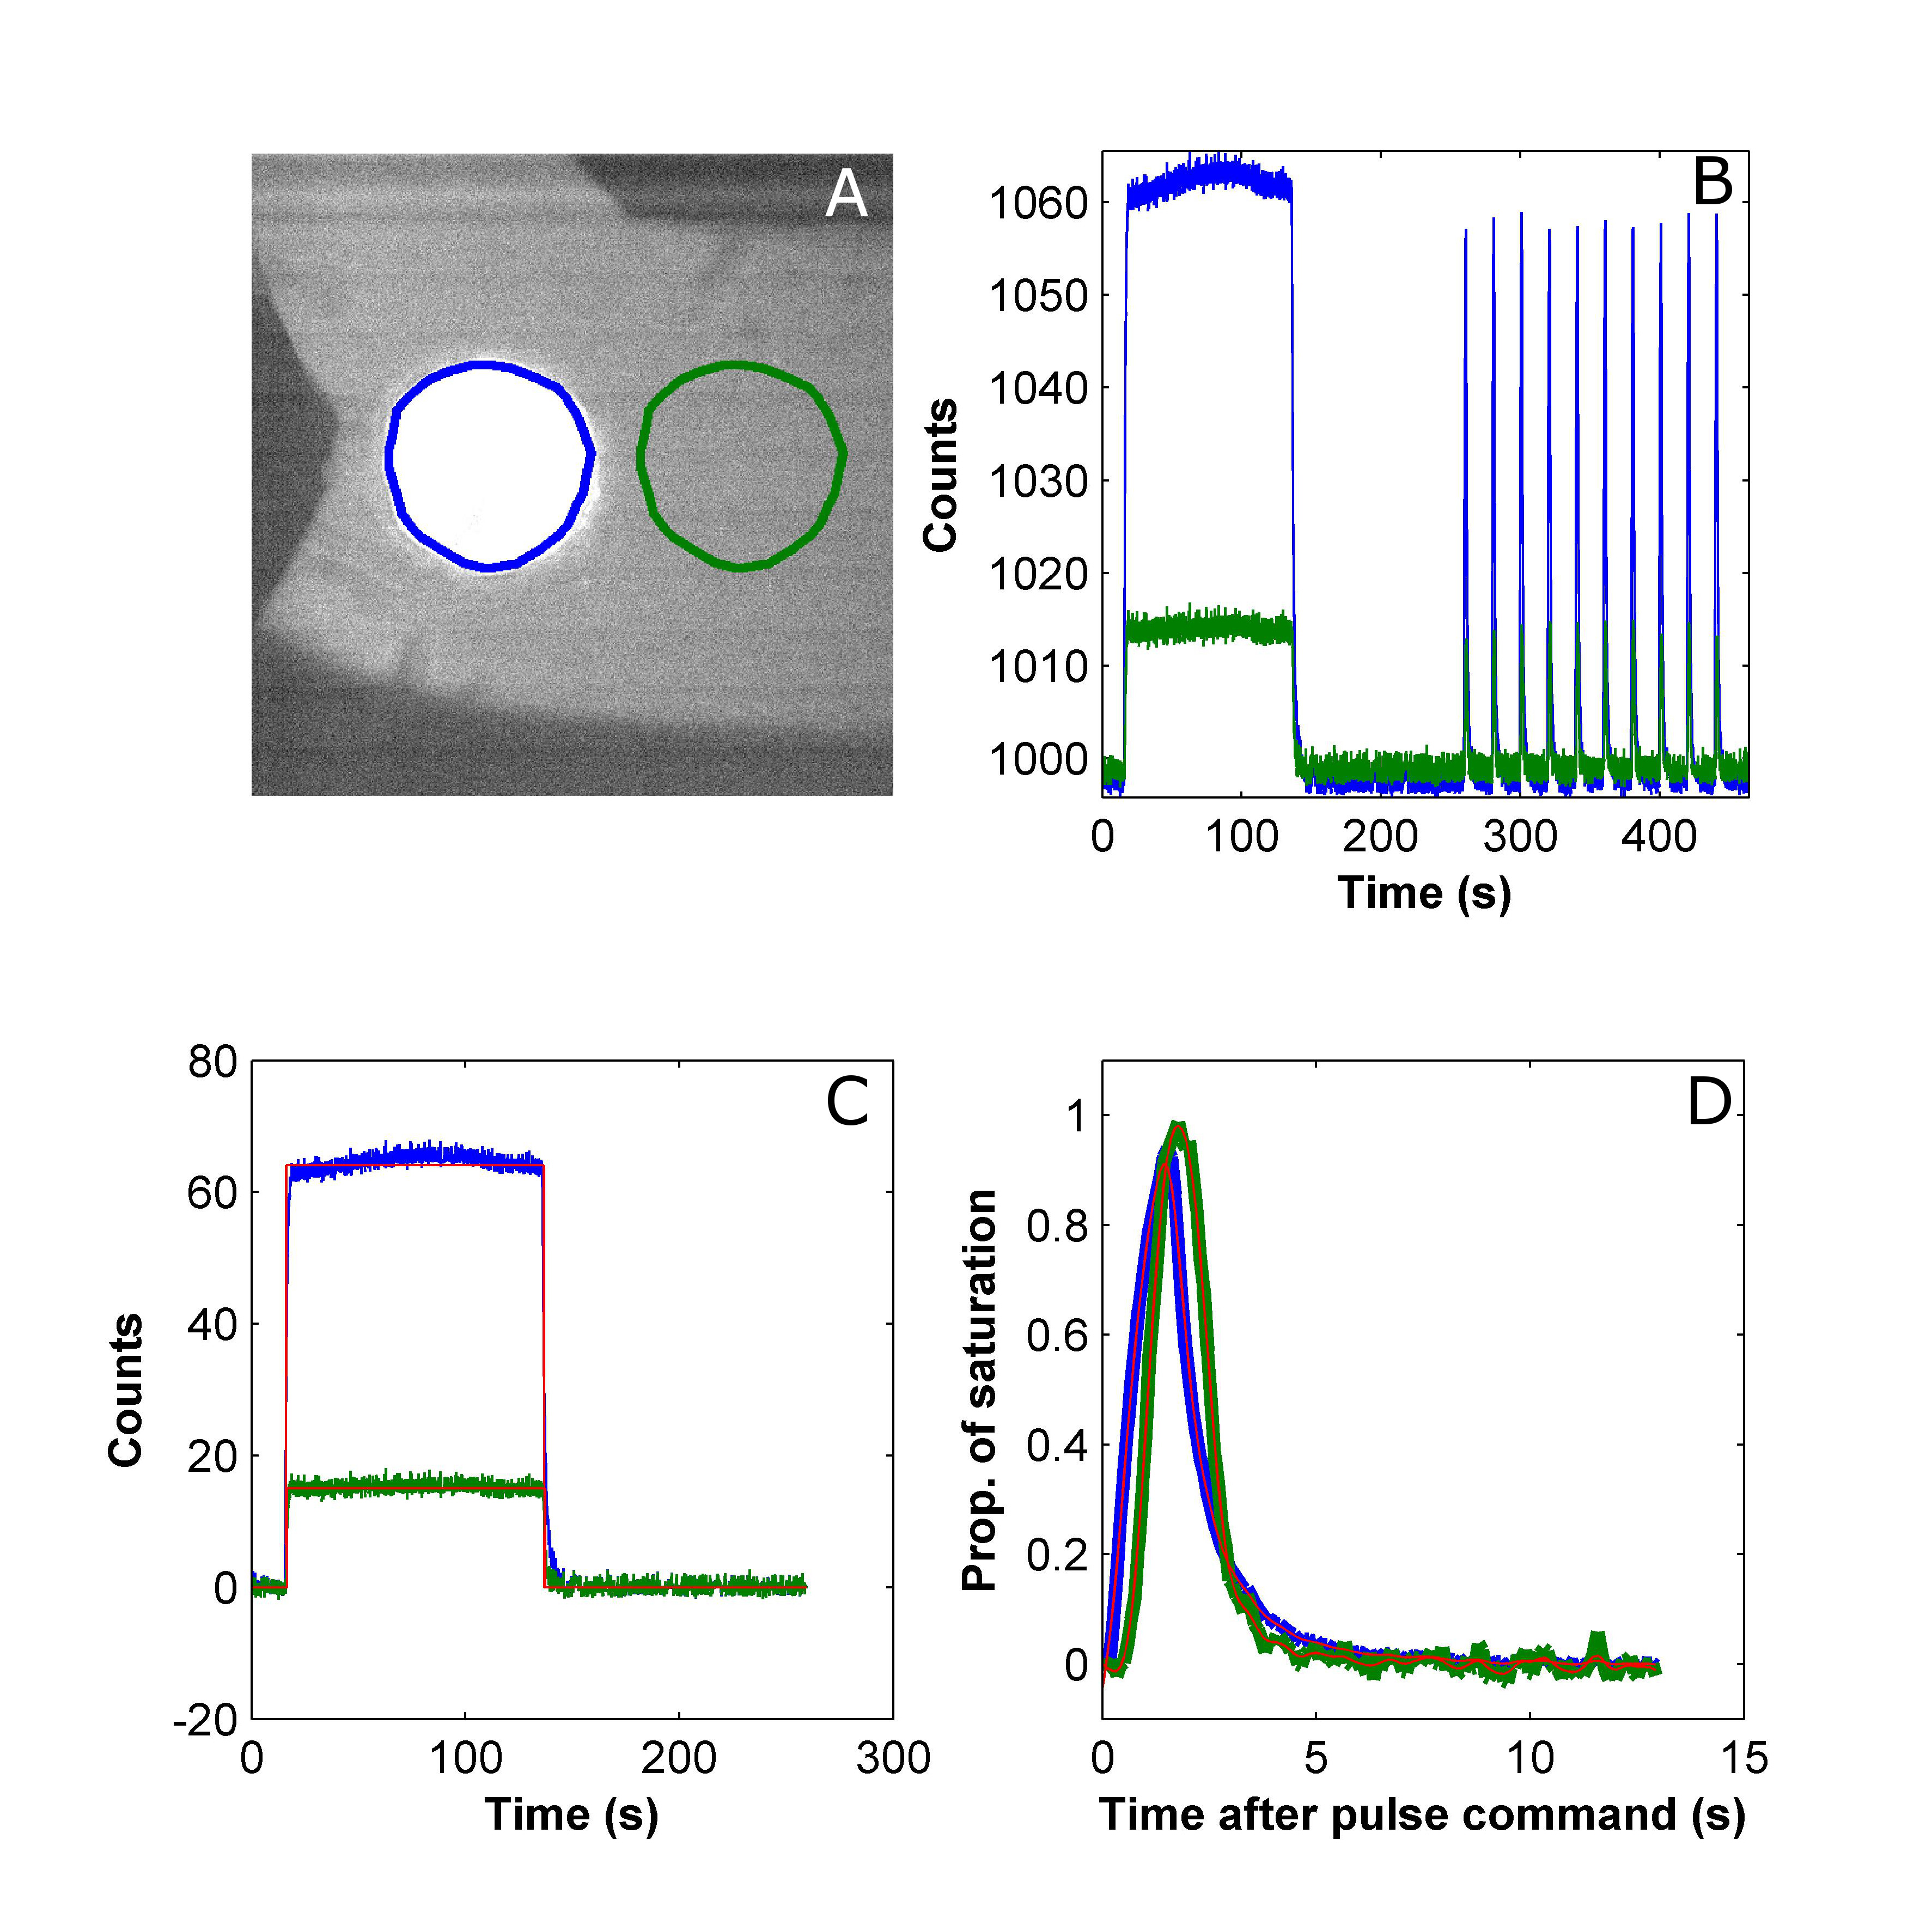
\includegraphics[width=15cm]{chapter6/figures/fluoAnalysis/fluoAnalysis.jpg}
       \caption[Analysis pipeline of fluorescence pulsing data]{\textbf{Fluorescence data is analyzed to determine the time course of ROI saturation.} (A) Sample regions of interest of identical shape. (B) Fluorescence traces extracted from the ROIs shown in A. The fluorescence pulsing experiments included an initial 2 minute period where the well was fully saturated with agonist to obtain a reference value. This was followed by 2 minutes of clearance and then 10 agonist pulses at 20 second intervals. (C) Square pulse fits to the saturation segment of the fluorescence trace after baseline removal. (D) Saturation time courses obtained by normalizing the fluorescence traces to the fitted saturation values in C and averaging over all 10 pulses.}
       \label{fig:pulses:fluoAnalysis}
  \end{figure}

\subsection{Numerical simulation of drug pulsing}
\label{sec:pulses:comsol}
We used the finite element solver software Comsol to generate a simulation of the pulse action in a 3D geometry closely mimicking the microwell devices. as reviewed in section \ref{sec:introduction:mufdDrugDelivery}, a hallmark of microfluidic technology is that the (relatively) low flow rates and the miniature dimensions dictate a laminar flow regime. In cases where the Reynold's number is \(<<\) 1 the inertial elements in the Navier-Stokes equation may be completely neglected resulting in a simplified model named creeping flow which includes only the hydrostatic and viscous terms \cite{fluidBook}. We calculated the Reynold's number for the the microwell devices of concern to be \(Re\approx 0.05\) and therefore used the `creeping flow' physics module to model the velocities in the device. We further employed the `transport of diluted species' module and coupled it to the velocity field from the former module to model the convective and diffusive transport of the agonist. We used a diffusion coefficient of a neurotransmitter sized molecule (\(400 \mu m^2\cdot s^{-1}\)). Geometry parameters were measured in microscope images and averaged over all the devices that participated in the visualization. The well height was measured prior to bonding using a clean room profiler. The channel height was calculated from the ratio between the fluorescent signal inside the well to that outside in locations fully saturated with agonist. This calculation resulted in a mean channel height of \(40\pm 3.7 \mu m\) which shows that the silicone tape becomes compressed by 20\% during the assembly process (as \(50 \mu m\) tape was used for the channel layer). A complete listing of the model parameter values is provided in appendix \ref{app:comsolParams}. The flow rates were applied as boundary conditions in the device ports. To properly model the switching of the flow rates we collected and averaged flow sensor data just after pulse commands. Figure \ref{fig:pulses:flowPulse} shows the averaged data from all 3 inline flow sensors (2 inlet and 1 outlet). The data show that following a flow switch the flow rates overshoot the set point and oscillate a few times. This is because the flow PID settings were purposefully adjusted to minimize the switch time at the cost of these minor oscillations. To model the flow switching, we disregarded the oscillations and assumed linear transition in flow rates between the set points over a switch time as in the original data (\(300 ms\), dashed line in figure \ref{fig:pulses:flowPulse}). We verified that this approximation did not impact the results in the model by also running simulations with the original flow data as input.

  \begin{figure}[!htb]
       \centering
       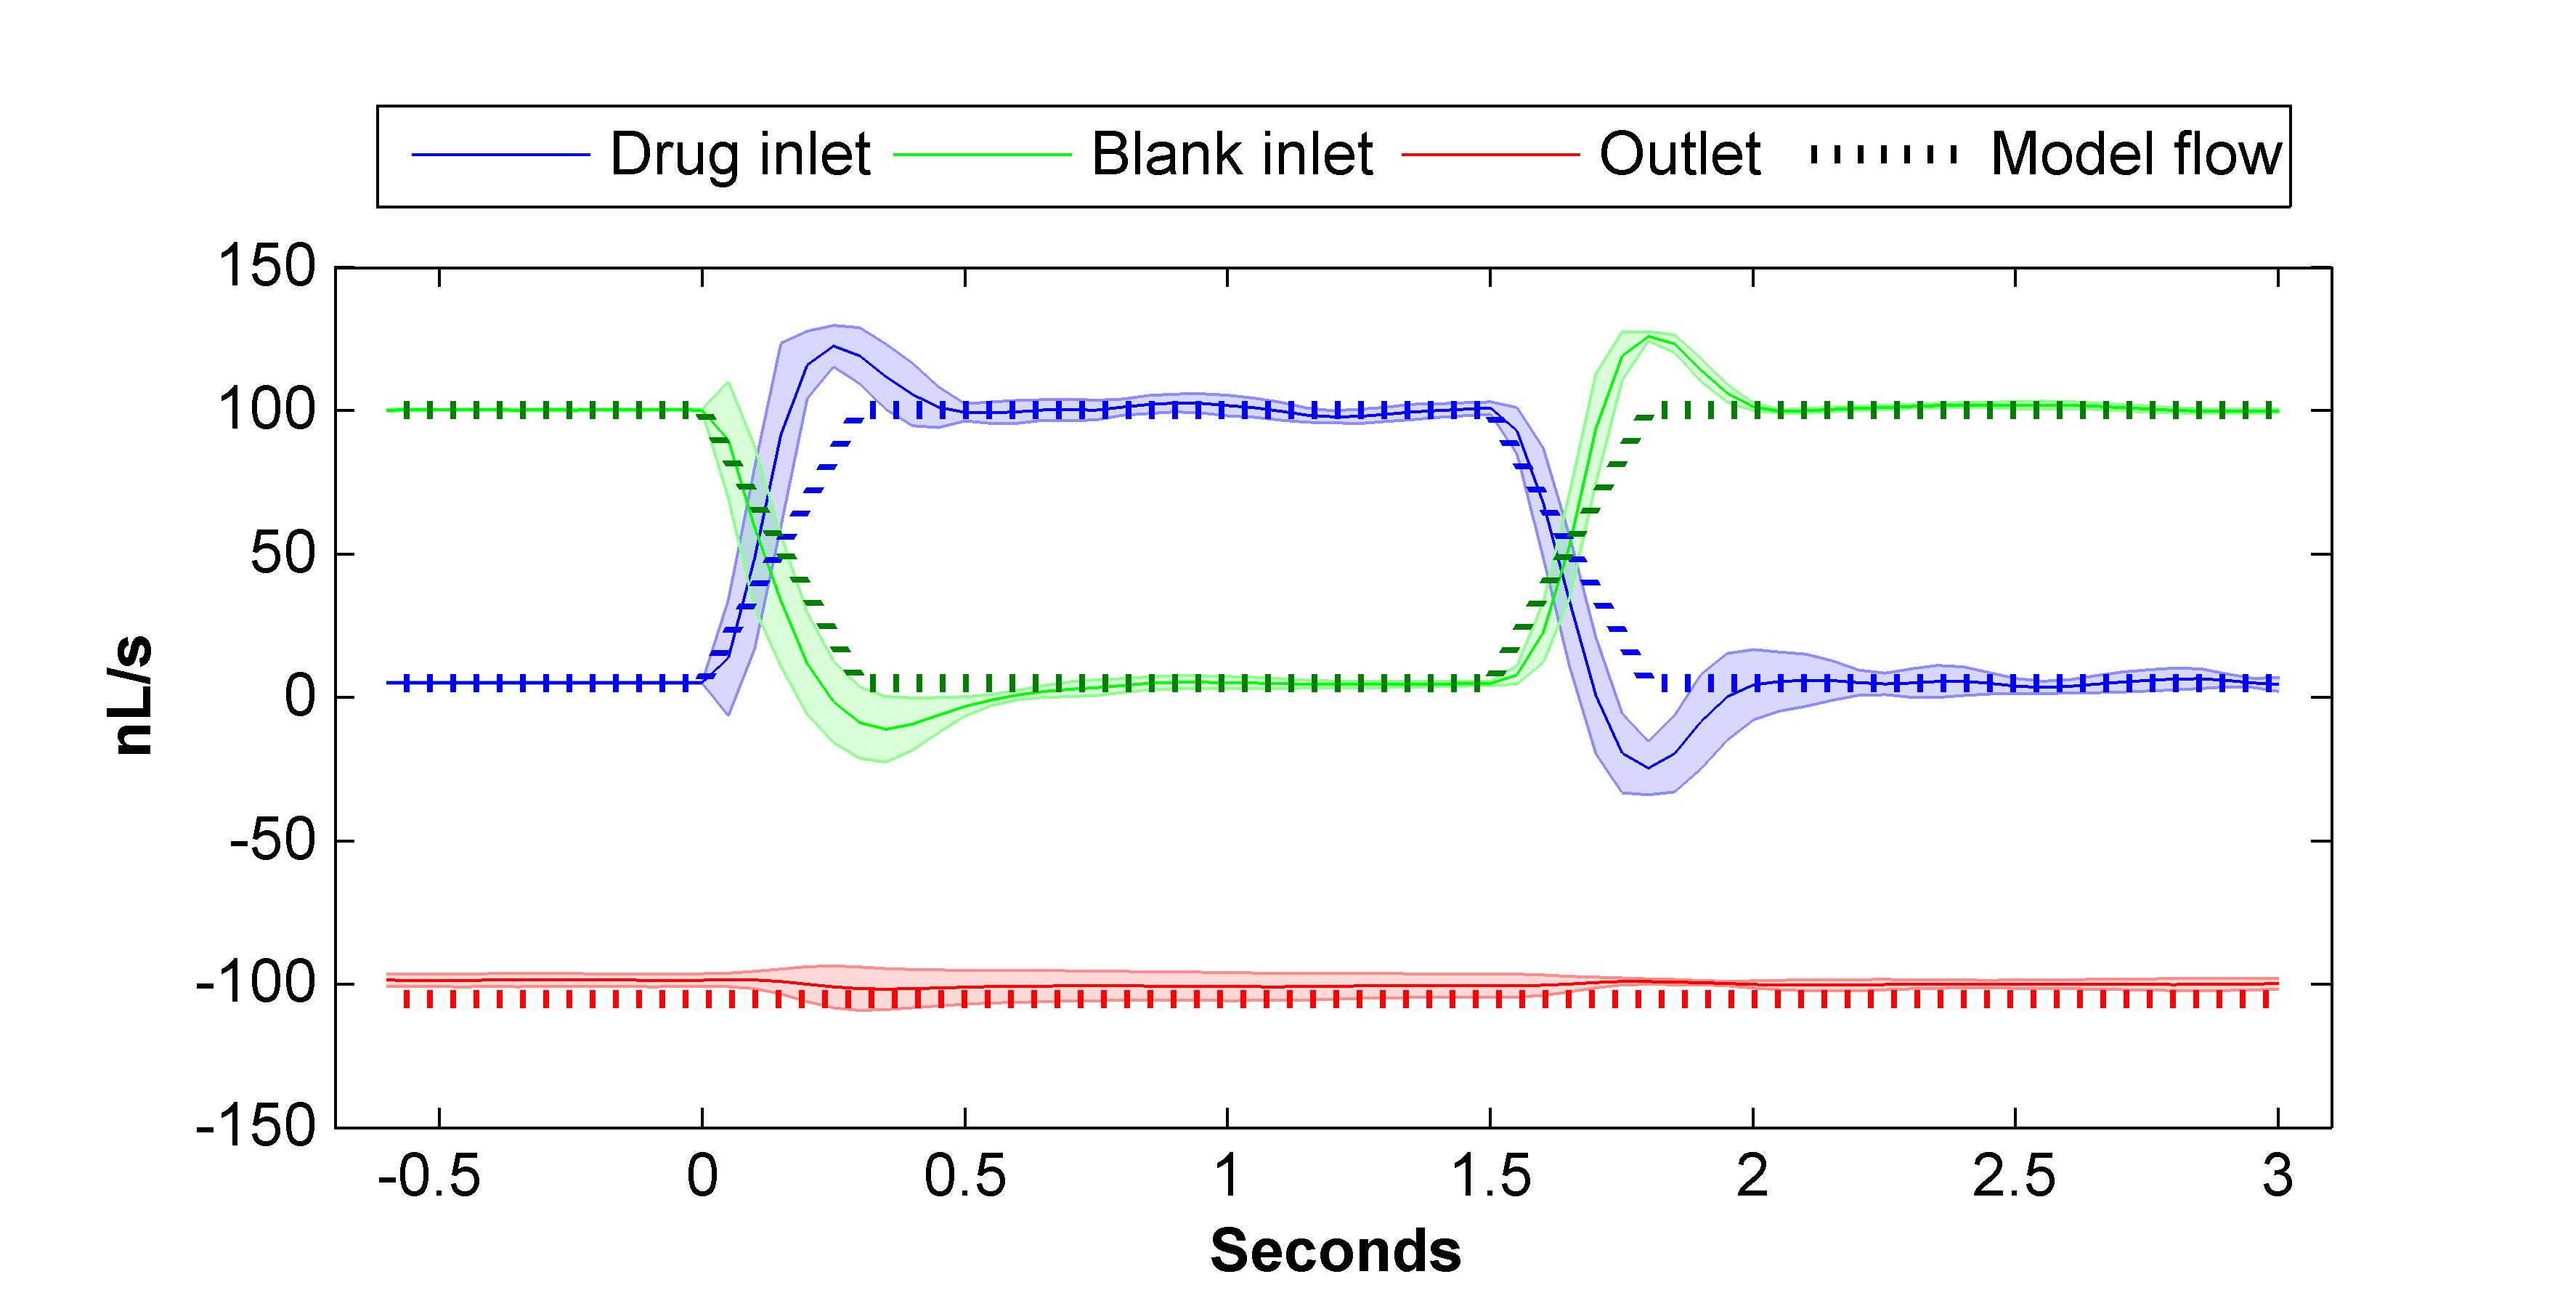
\includegraphics[width=15cm]{chapter6/figures/flowPulse/flowPulse.jpg}
       \caption[Measured and model flow rate switches during an agonist pulse]{\textbf{Flow switching was modeled as a linear transition between the set flow rates.} The input flow rates are set to \(100\) and \(5 nL\cdot s^{-1}\) at baseline. To generate the agonist pulse the flow rates are flipped for 1.5 seconds. The measurements show that the flow rates oscillate briefly and are not completely symmetric in their switch kinetics. Nevertheless, modelling the switch as a linear transition between the set points over \(300ms\) provided a good match between model and experiment. Shaded areas represent standard deviation. Flow sensor data is based on 4 devices with 10 pulses each.}
       \label{fig:pulses:flowPulse}
  \end{figure}

To validate the model through comparison to the experiments, we chose 3 equally spaced locations of measurement within the microwell along a line at a \(45\degree\) angle from the longitudinal channel axis (figure \ref{fig:pulses:modelValidationIllustration}). We extracted saturation time course as described in the previous section from ROIs of \(10\times 10\) pixels centered at these locations. These were compared to the predicted mean concentration along vertical lines at the same locations in the model. The data show a striking resemblance between the model generated and the experimental time courses, particularly in the temporal features (e.g., the asymmetry between the rising and decay phases). A certain discrepancy between model and experimentation is observed at the spatial location farthest from the agonist port where the concentration peak was lower in the latter case.


  \begin{figure}[!htb]
       \centering
       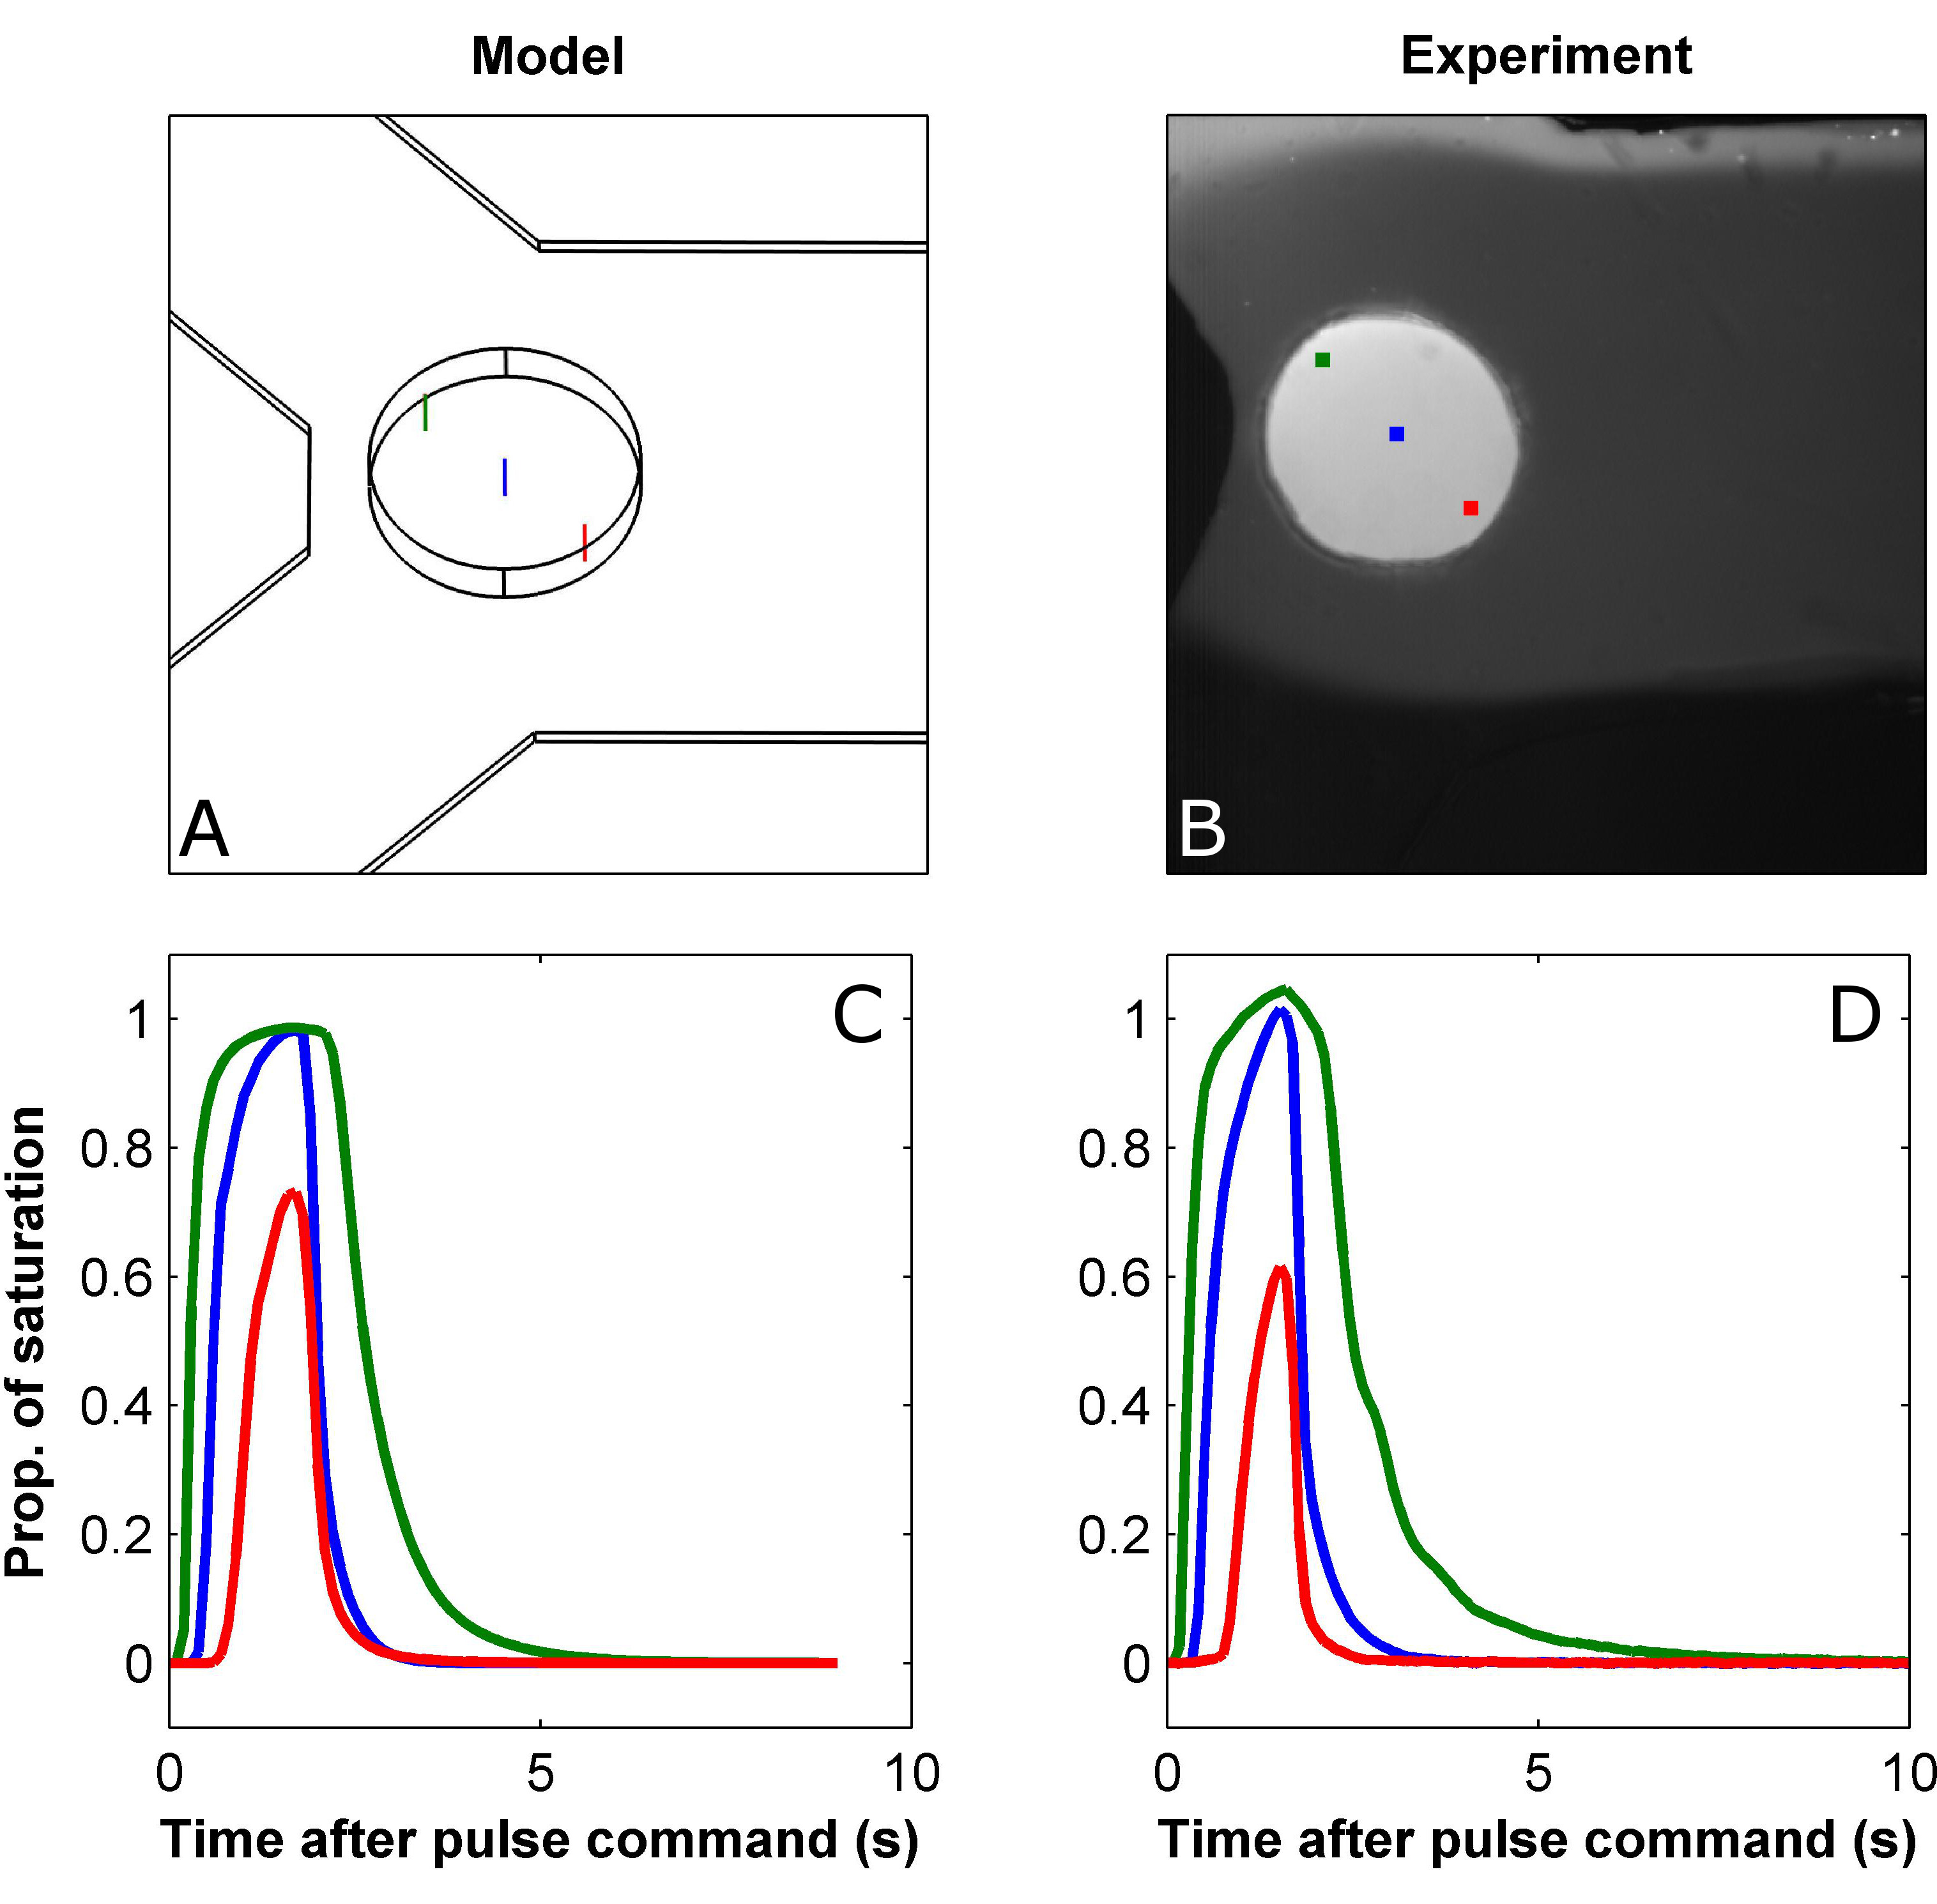
\includegraphics[width=12.8cm]{chapter6/figures/modelValidationIllustration/modelValidationIllustration.jpg}
       \caption[Comparison between model predictions and measured agonist time course]{\textbf{The model captures the fine kinetic details of agonist transients in different locations across the microwell.} (A) Model geometry generated in Comsol and showing the three lines of examination. (B) Image of device during a fluorescence visualization showing 3 points of examination matching the lines in A. The agonist concentration averaged across the model lines is considered proportional to the fluorescence at the corresponding point because of the low Z axis resolution of the wide field microscopy. (C) Concentration traces averaged over the lines shown in A (agonist concentration in the model is arbitrarily set to 1). (D) Normalized saturation traces at the points shown in B extracted as described in section \ref{sec:pusling:fluo}.}
       \label{fig:pulses:modelValidationIllustration}
  \end{figure}

  To further compare the model prediction to the measurements we present an overlay of the model data on averaged measurements in figure \ref{fig:pulses:modelValidation}. This figure also shows the standard deviation of the experimental measurements which probably reflects the variability in device fabrication. This comparison shows a striking match between model and measurements in the onset of the rising phases of concentration pulses. This shows that the model predicts the travel time across the microwell well. On the other hand, the experimental time courses in all 3 spatial locations seemed sluggish as compared to the model with both rise and decay times somewhat longer in the former. We suspect that the sluggishness is related to the presence of the bubble traps in the flow lines (see section \ref{sec:methods:flow}). These bubble traps are essentially PDMS devices with large cavities that are meant to collect bubbles which may interfere with the flow. Because of their elasticity, the traps function as capacitive elements with respect to pressure changes and therefore dampen sharp transitions in the flow rates (e.g., during an agonist pulse). Thus further improvements to the accuracy of the model may be achieved by measuring the flow rates down the line from the bubble traps or by changing them to a stiff material. Nevertheless, even as is, the model's predictions are within one standard deviation from the measurements. We therefore argued that further improvements would only provide marginal benefit and decided to continue with the model as is.

  \begin{figure}[!htb]
       \centering
       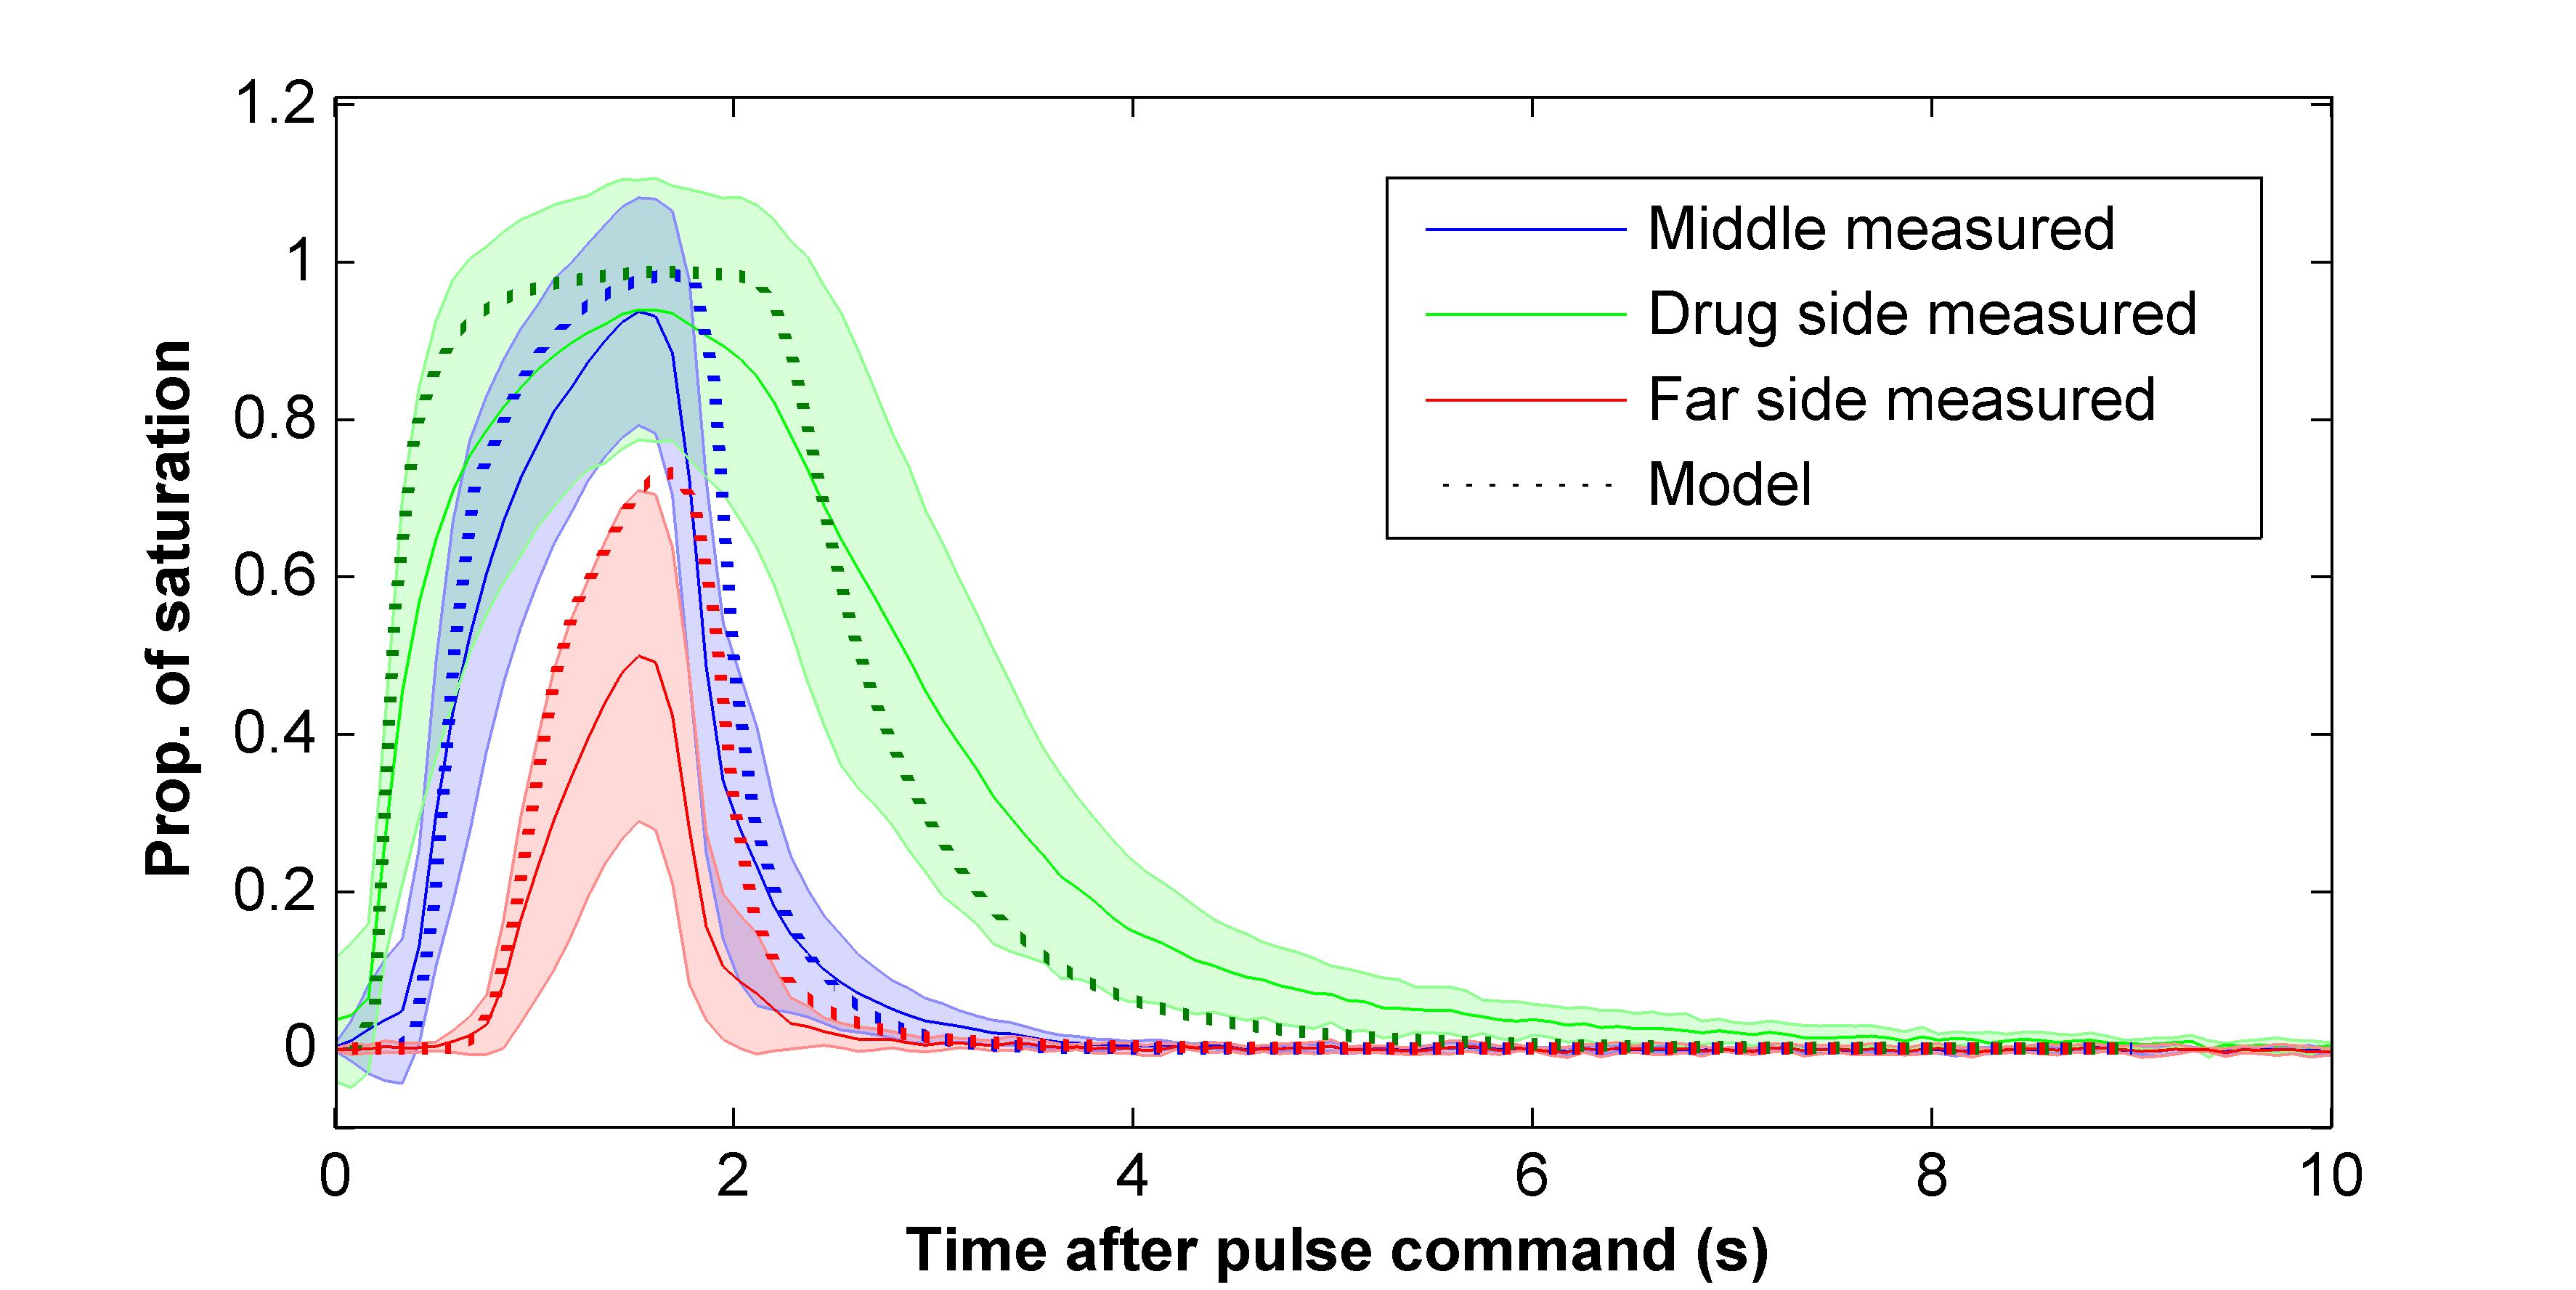
\includegraphics[width=15cm]{chapter6/figures/modelValidation/modelValidation.jpg}
       \caption[Comparison between model predictions and measured agonist time course including variability between devices]{\textbf{Measured transients are in good agreement (albeit slightly more sluggish) with the model.} Overlay of the model and measured transient data at 3 locations in the microwell as indicated in figure \ref{fig:pulses:modelValidationIllustration}. Experimental transients are averaged over n=5 devices. Shaded area represents standard deviation.}
       \label{fig:pulses:modelValidation}
  \end{figure}

  The establishment of the finite element model provides us with estimates of detailed agonist concentrations in the 3D volume of the device. This allows us to generate detailed agonist distributions around the cells (the microwell bottom) during an agonist pulse (figure \ref{fig:pulses:concentrationsChart}). This data shows that the cells are already exposed to significant concentrations of agonist within a second from the pulse command. This type of information can be consulted for applications with constraints on the concentration distribution across the tissue. At present there is no clear cut information regarding how evenly neuromodulators are distributed in the tissue during a transient so we will restrict discussion to the concentration time course averaged over the entire well area from now on.

  Figure \ref{fig:pulses:glutamatePulses} shows the averaged concentration time course during an agonist transient in devices with \(120 \mu m\) deep microwells. The transient lasts for about 5-6 seconds before decaying back to baseline levels. Data from amperometric dopamine sensing studies show that reward associated dopamine transients can last between 1 and 7 seconds, depending on the the brain region under examination \cite{mittleman2008cerebellar,phillips2003subsecond,venton2003real}. This places the transients shown here on the slow end of the spectrum and they can be taken to represent release in a brain region with a low density of dopaminergic innervation where the molecules linger in the extra cellular space for several seconds before being fully uptaken. Other neuromodulatory systems generate transients in the same range of time scales \cite{dankoski2015monitoring,dugast2002vivo,sarter2009phasic}. Another distinctive difference between the transient generated by our system and amperometric data is the rise time. In \textit{in vivo} conditions the concentration transient is generated by a synchronized quantal release event occurring in many synaptic sites across the tissue. This process generates sharp concentration increases which normally peak within less than a second. In the case of our interface shifting approach the rise time depends on the rate at which the interface is swept across the microwell, which may be controlled by adjusting the flow rate. The purpose of this work was not to account for specific kinetic details of the neuromodulator transient but to show that the physiological range of time scales may be achieved. Also, it not clear which of the features is specifically critical to the functional aspects of the phasic neuromodulatory signalling. However, this does not mean that the interface shifting methods is not conducive to generating transients with specific features. To demonstrate this, the next section will show that by manipulating device and flow parameters faster time scales may be achieved. These will be compared to amperometric data from our collaborators.

  \begin{figure}[!htb]
       \centering
       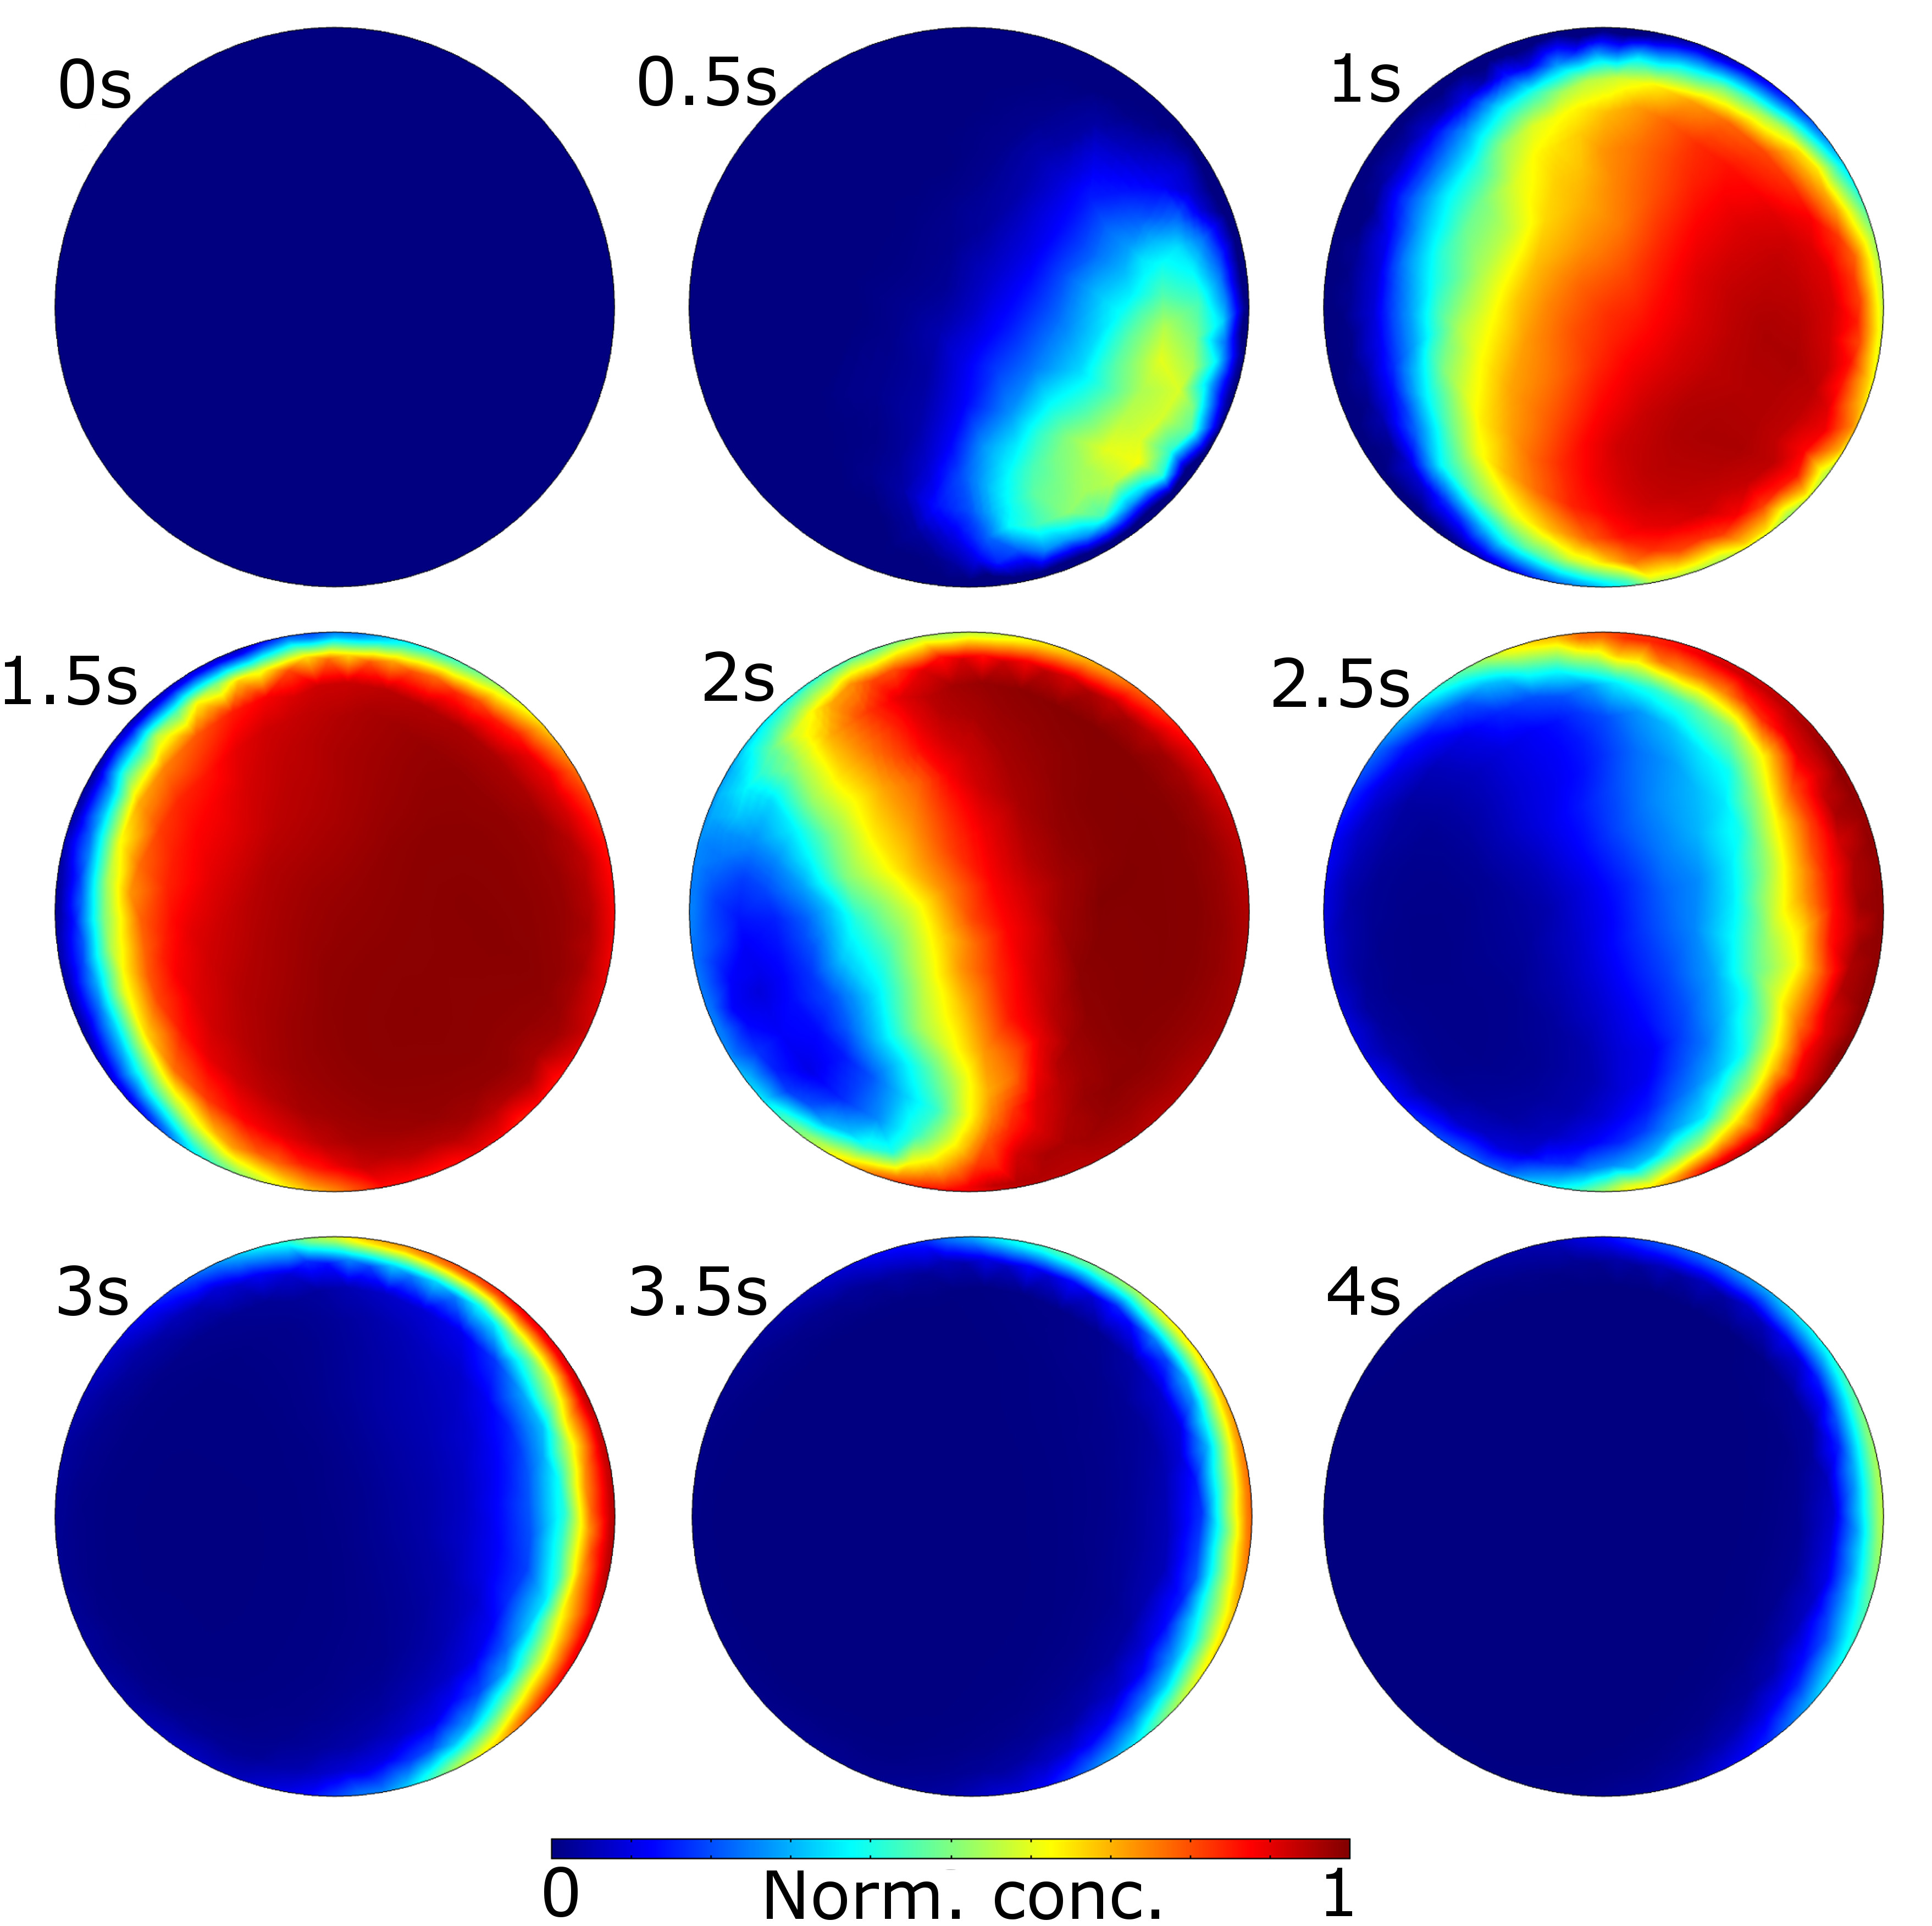
\includegraphics[width=15cm]{chapter6/figures/concentrationsChart/concentrationsChart.jpg}
       \caption[Spatial distributions of agonist concentration in the microwell during a pulse]{\textbf{The microwell is widely inhabited with agonist within a second from the pulse command}. Model derived agonist distributions across the microwell (in a parallel plane \(6 \mu m\) from the bottom surface) at fixed time points following a pulse command. Note that in this outline the agonist and blank inlets are located at the bottom (right and left, respectively).}
       \label{fig:pulses:concentrationsChart}
  \end{figure}

\subsection{Shortening of the transient time scales by changing microfluidic parameters}
\label{sec:pulses:fastPulses}
We argued that transient time may be shortened by increasing the flow rate and by making the microwell shallower. Both of these changes are expected to reduce the time taken to fill up the microwell and subsequently empty it from the agonist. However, reduction in the fill time also needs to be accommodated by a reduction in the pulse width (the duration of time that the flow rates are held in pulse mode during the pulsing sequence, see section \ref{sec:pusling:fluo}). A correct selection of the pulse width is critical as holding it for too long will lengthen the transient and cutting it short may prevent the agonist from reaching all of the cells. To reconcile these contradictory requirements we defined the optimal pulse width for a given flow rate / geometry to be the shortest pulse where the agonist concentration in at least 95\% of the microwell bottom area had reached at least 95\% of the concentration in the input stream. The reason for not requiring 100\% saturation is that we found that the very final stages of filling process take a disproportionately long time compared to the earlier ones and so demanding a complete fill is counterproductive in the given scenario. In order to find the optimal pulse width which complies with this criteria we ran numerical simulations of agonist pulses with a range of pulse widths (while fixing all other parameters). For each of these runs we computed the time course of the microwell fill. This was taken as the proportion of the well surface (i.e., a parallel plane, \(6\mu m\) from the well bottom) where the concentration had reached at least 95\% of the input. The maximal fill values were used to generate a plot of maximal fill as a function of pulse width which was normally monotonically increasing. The optimal pulse width was finally taken as the intersection of the plot with 95\% fill. This process is demonstrated in figure \ref{fig:pulses:reducedTimeScales} A-B.

Using the above procedure, we simulated the optimal agonist transients for flow rates between \(100-600 nl\cdot s^{-1}\) and a well depth of \(10\mu m\). These transients are shown in figure \ref{fig:pulses:reducedTimeScales} D. These data show even for the flow rate used in the other sections, \(100 nl\cdot s^{-1}\), the transient is appreciatively narrower (compare with figure \ref{fig:pulses:glutamatePulses} B) owing to the use of the shallow well. The same panel also shows a dopamine transient obtained through amperometric measurements in the rat striatum. These data were provided courtesy of Dr. James McCutcheon from The University of Leicester. As the striatum is the one the brain regions with the highest density of innervating dopamine terminals the amperometry-measured transient probably represents the fastest in the time scale range. Nevertheless, as shown by the comparison the microfluidics can readily match these time scales and even exceed them. This demonstrates that the interface shifting paradigm can generate phasic neuromodulator signalling at any physiologically-relevant time scale and highlights the usefulness of using fluid dynamics numerical simulation in calibrating the microfluidic parameters.


  \begin{figure}[!htb]
       \centering
       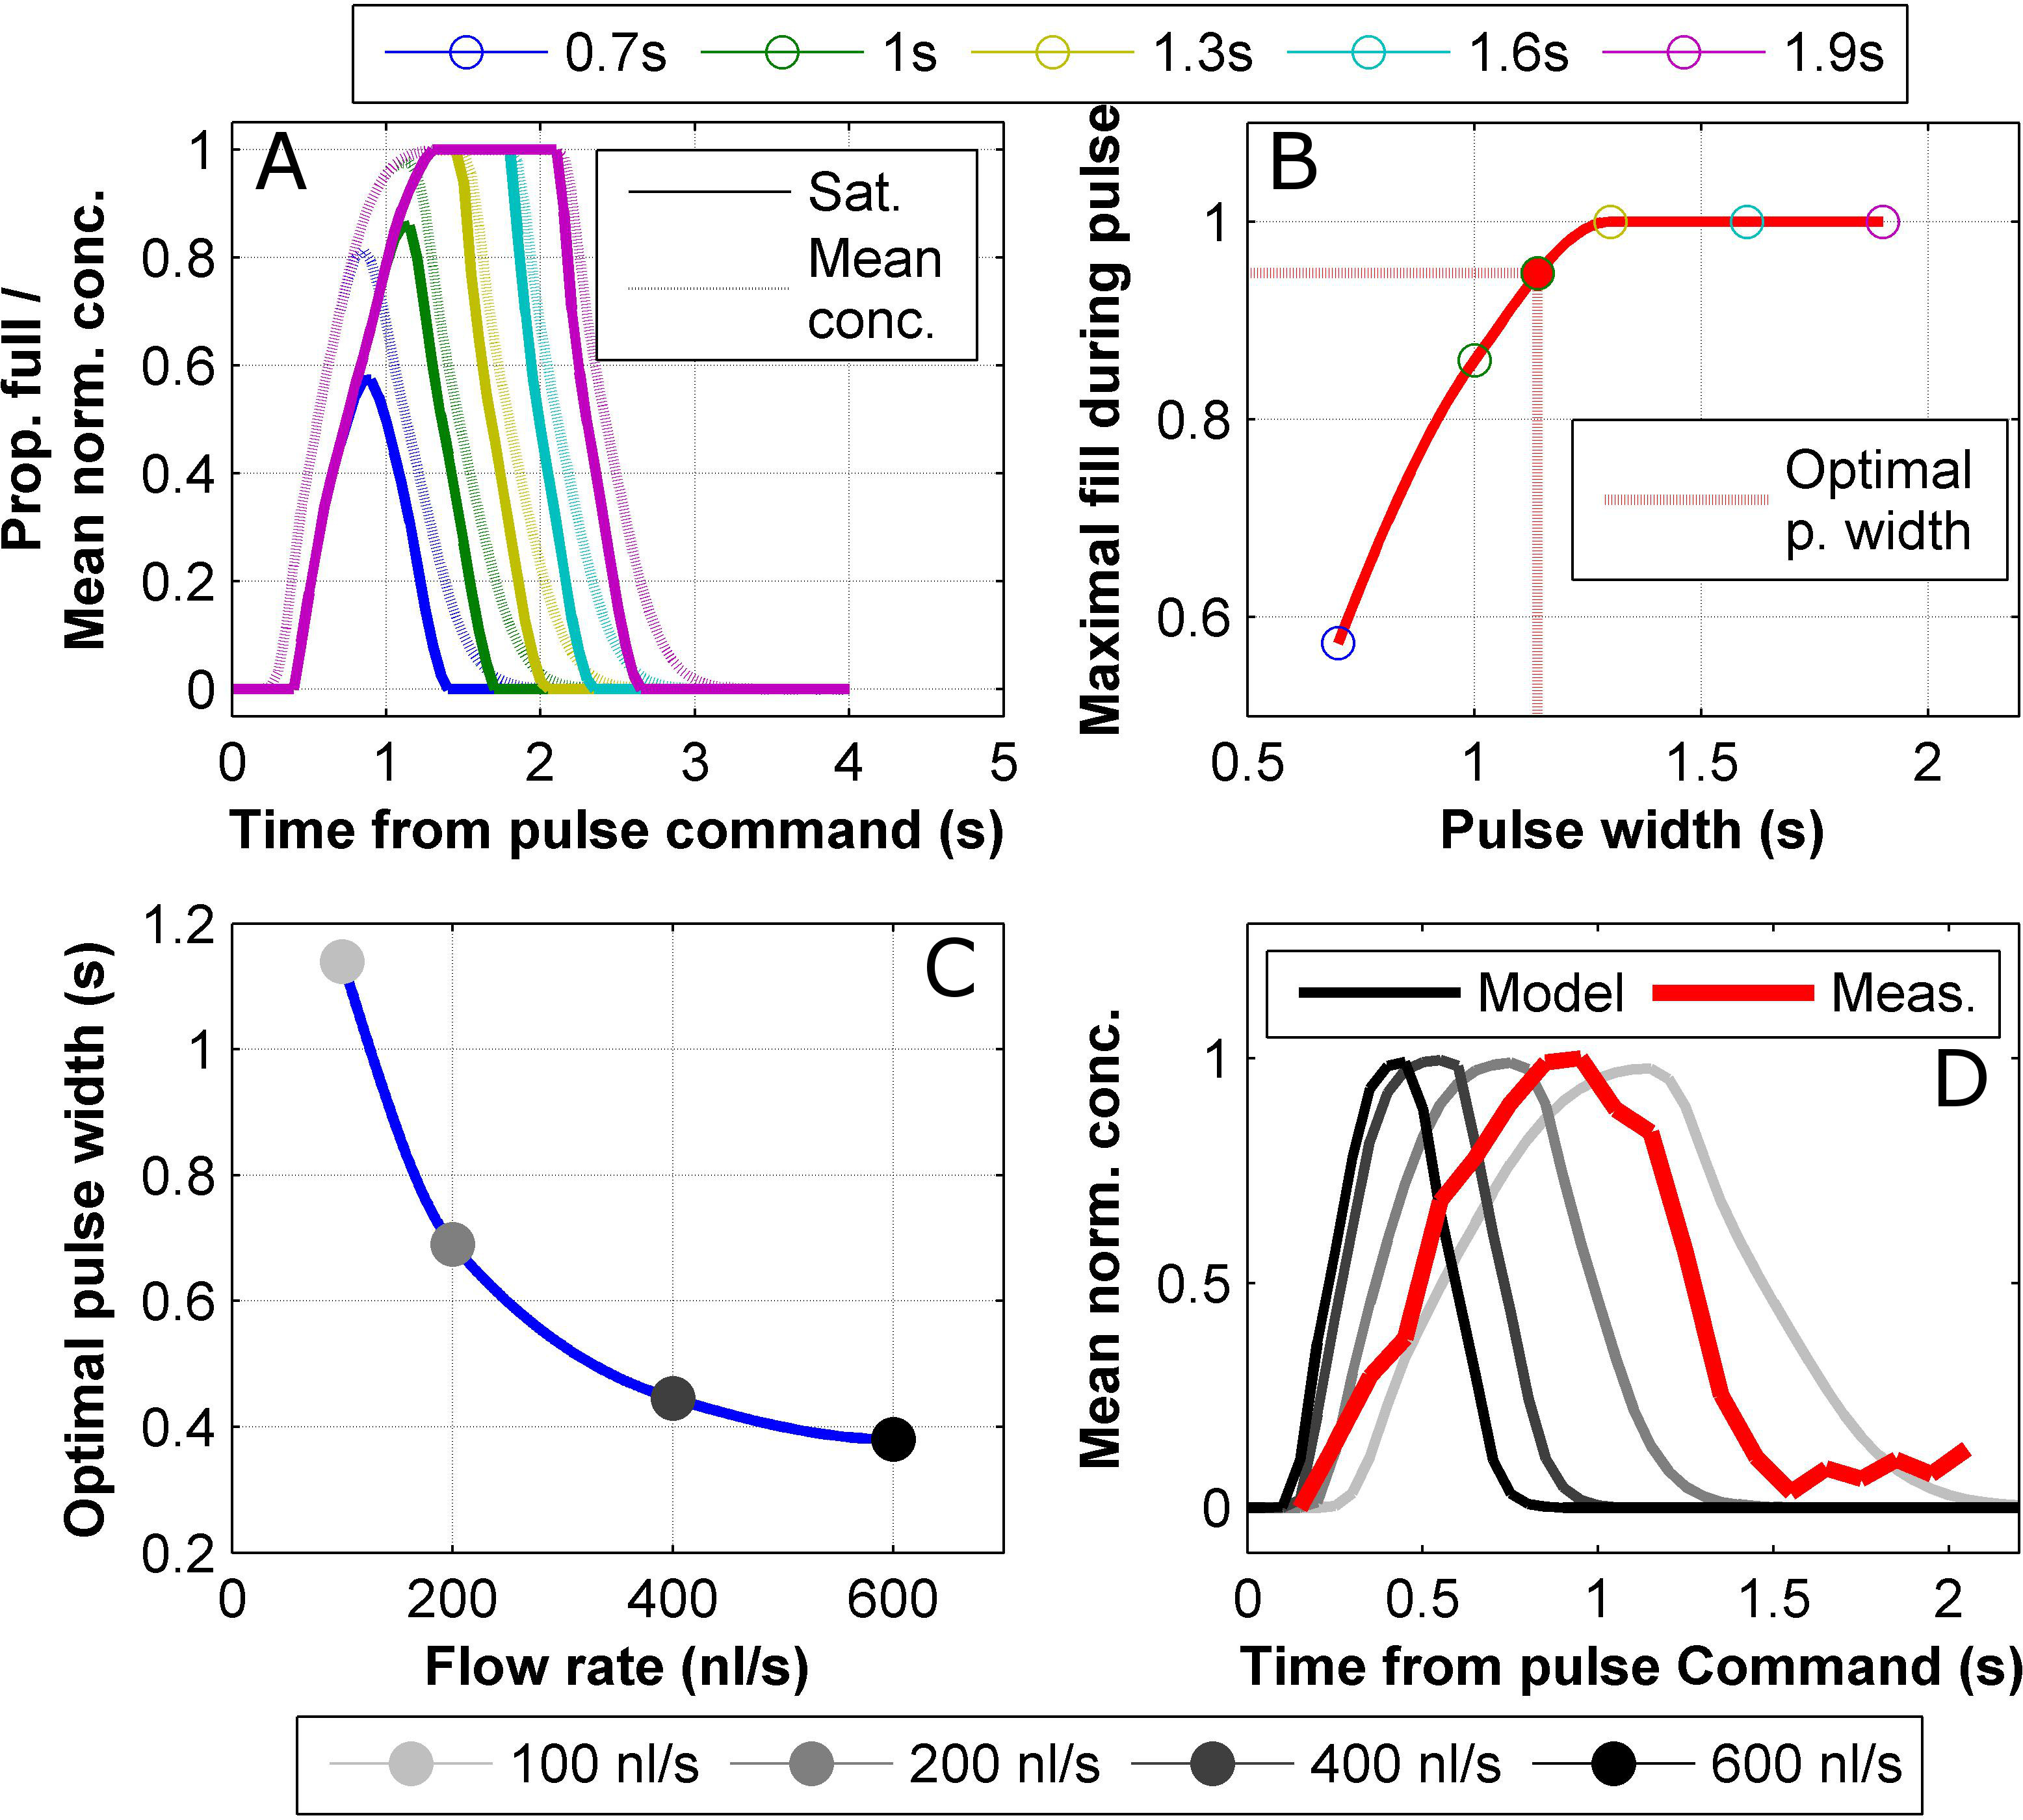
\includegraphics[width=13.17cm]{chapter6/figures/imporvedTimeScales/FlowRateDeterminedTimeScales.jpg}
       \caption[Shortening of the agonist transient time scales by changing the microfluidic parameters]{\textbf{By increasing the flow rates and using a shallow microwell, transients may be generated that are narrower than those observed in the striatum}. (A) Time course of well filling during agonist pulses simulated at several pulse widths and a flow rate of \(100 nl\cdot s^{-1}\) in a \(10 \mu m\) deep microwell. Time course of agonist concentration averaged over the well surface is also shown for information. Precise definition of proportion fill measure is given in the text. Pulse widths longer than the time needed to completely fill the well (transients with a prolonged plateau) or ones too short to achieve complete filling are suboptimal. (B) Maximal well fill as a function of pulse width. Open circles are the maxima of the curves shown in A. Optimal pulse width is the one generating 95\% fill. Red curve is a piecewise cubic hermite interpolation of the open circles. (C) Optimal pulse width as a function of flow rate computed as shown in A-B. \(10\mu m\) deep microwells were used in all cases. Blue curve is an interpolation of the data points as in B. (D) Optimal agonist concentration transients averaged over well surface for several flow rates. Also shown is a dopamine transient measured via amperometry in rat striatum and presented after baseline correction and normalization to it own peak. These data were provided courtesy of Dr. James McCutcheon of The University of Leicester.}
       \label{fig:pulses:reducedTimeScales}
  \end{figure}

\section{Glutamate pulsing}
To further demonstrate the ability of the system to generate a biological response in the predicted time scales we made several recordings where pulsing was performed with \(100 \mu M\) glutamate. Figure \ref{fig:pulses:glutamatePulses} shows an example PSTH from one culture as well one averaged over 3 such experiments. The predicted glutamate concentration transients averaged over the well bottom is overlayed for reference. The data show that the cultures reacted to the glutamate transients with a burst of action potentials starting \(\approx 500 ms\) after the pulse command. The spiking activity returned to the baseline levels after \(\approx 6\) seconds, in good agreement with the predicted time scales of the agonist transients. At first glance, the activity transient seems not to comply well with the predicted glutamate concentration time course because the spiking activity surge mostly terminated before the glutamate was washed away. However, in interpreting these results one should take receptor desensitization into account.

The time course of the activity transient was evidently composed of two parts: an initial intense phase consisting of a sharp increase in the firing rates which is significantly shorter lived than the agonist transient and an ensuing phase of sustained firing at much lower levels (but still evidently above baseline). Ionic glutamate receptors are known to undergo rapid desensitization under prolonged exposure to the agonist. In particular, the AMPA receptor desensitizes completely after just a few milliseconds \cite{trussell1993desensitization}. The NMDA receptor desensitizes more slowly \cite{mayer1985action} and not completely, as it was shown to produce tonic currents in the sustained presence of glutamate \cite{sah1989tonic}. Thus it is plausible that the initial intense activity phase is associated with a temporary opening of both AMPA and NMDA channels which deactivate quickly, leaving just a partial NMDA associated depolarizing current responsible for the second phase. Moreover, one should take into account the observed measure is that of complex network activity which probably involves many mechanisms, synaptic or intrinsic, to control excitability (e.g., feedback inhibition). Thus, the shorter time scales of the first phase as compared to those of the predicted agonist concentration should therefore not be taken as undermining the model validity.

    \begin{figure}[h]
       \centering
       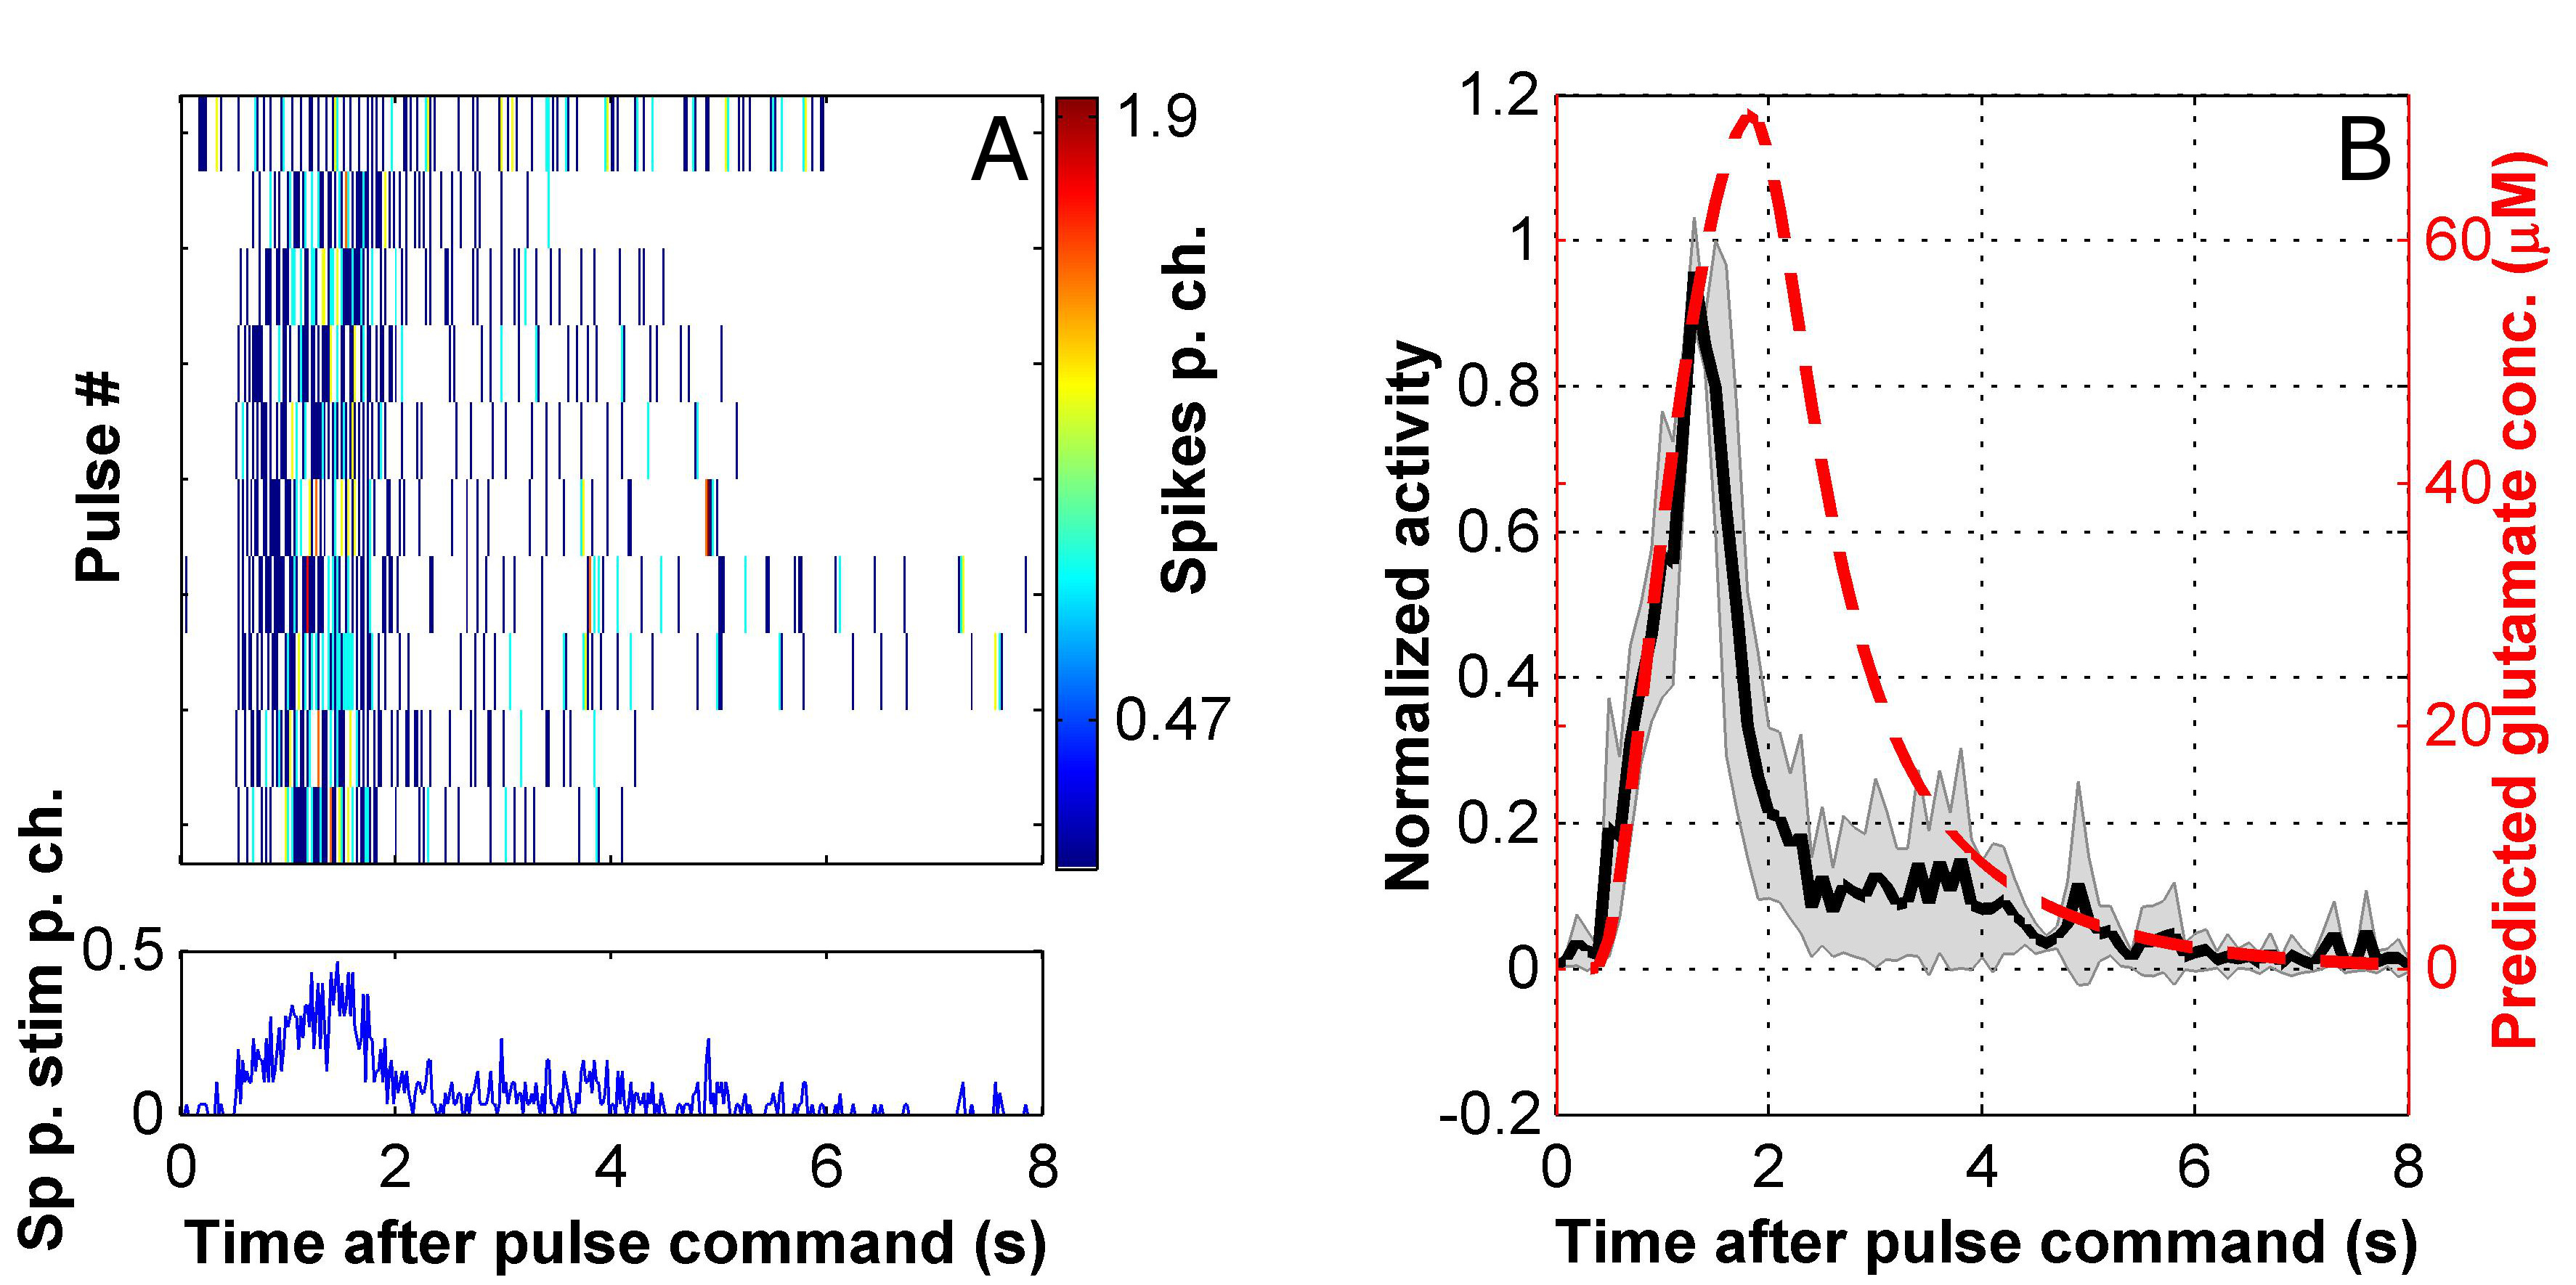
\includegraphics[width=15cm]{chapter6/figures/glutamatePulses/GlutamatePulsingAvg.jpg}
       \caption[Microculture electrical responses to glutamate pulses]{\textbf{The culture responds to glutamate pulses with intense firing events of length matching the predicted agonist time course.} (A) Example post pulse rasters and time histogram showing the responses to 10 glutamate pulses applied at 20 second intervals. (B) Averaged post pulse time histogram (PPTH) overlayed with the predicted glutamate time course (spatial average of the concentration across a parallel plane \(6\mu m\) from the well bottom). PPTH is average of data from n=3 microcultures. Shaded area represents standard deviation. These experiments were conducted in devices with \(120\mu m\) deep microwells.}
       \label{fig:pulses:glutamatePulses}

   \end{figure}


\section{Dopamine pulsing}
\label{sec:pulsing:dopamine}


In previous sections, we have demonstrated that our realization of the interface shifting paradigm can generate agonist transients at time scales of phasic neuromodulatory signalling. What remains to be demonstrated is that the microcultures sustain a stable network activity under flow (i.e., that the macroculture results of chapter \ref{chap:activityAndFlow} are transferrable to the microcultures), that the pulsing action does not perturb the activity, and that the cells are responsive to neuromodulators, even under flow. To address these gaps and finalize the validation of the system, we designed an experimental paradigm inspired by the Izhikevic thought experiment (section \ref{sec:introduction:izi}). We placed microcultures under flow while being subjected to electrical stimulations that induce a network reverberatory response. During a defined epoch, the electrical stimulations were coupled to pulses of dopamine (or blank media). The stimulation responses before, during and after the pulsing were monitored for short and long term effects of the pulse action and the dopamine coupling. The experimental paradigm is further outlined in figure \ref{fig:pulses:expOutline}. Beyond the validation of the system, the results of this section bear relevance to the results of the plasticity induction experiment carried out in section \ref{sec:activity:plasticityProtocol}, which will be discussed as well.

  \begin{figure}[h]
       \centering
       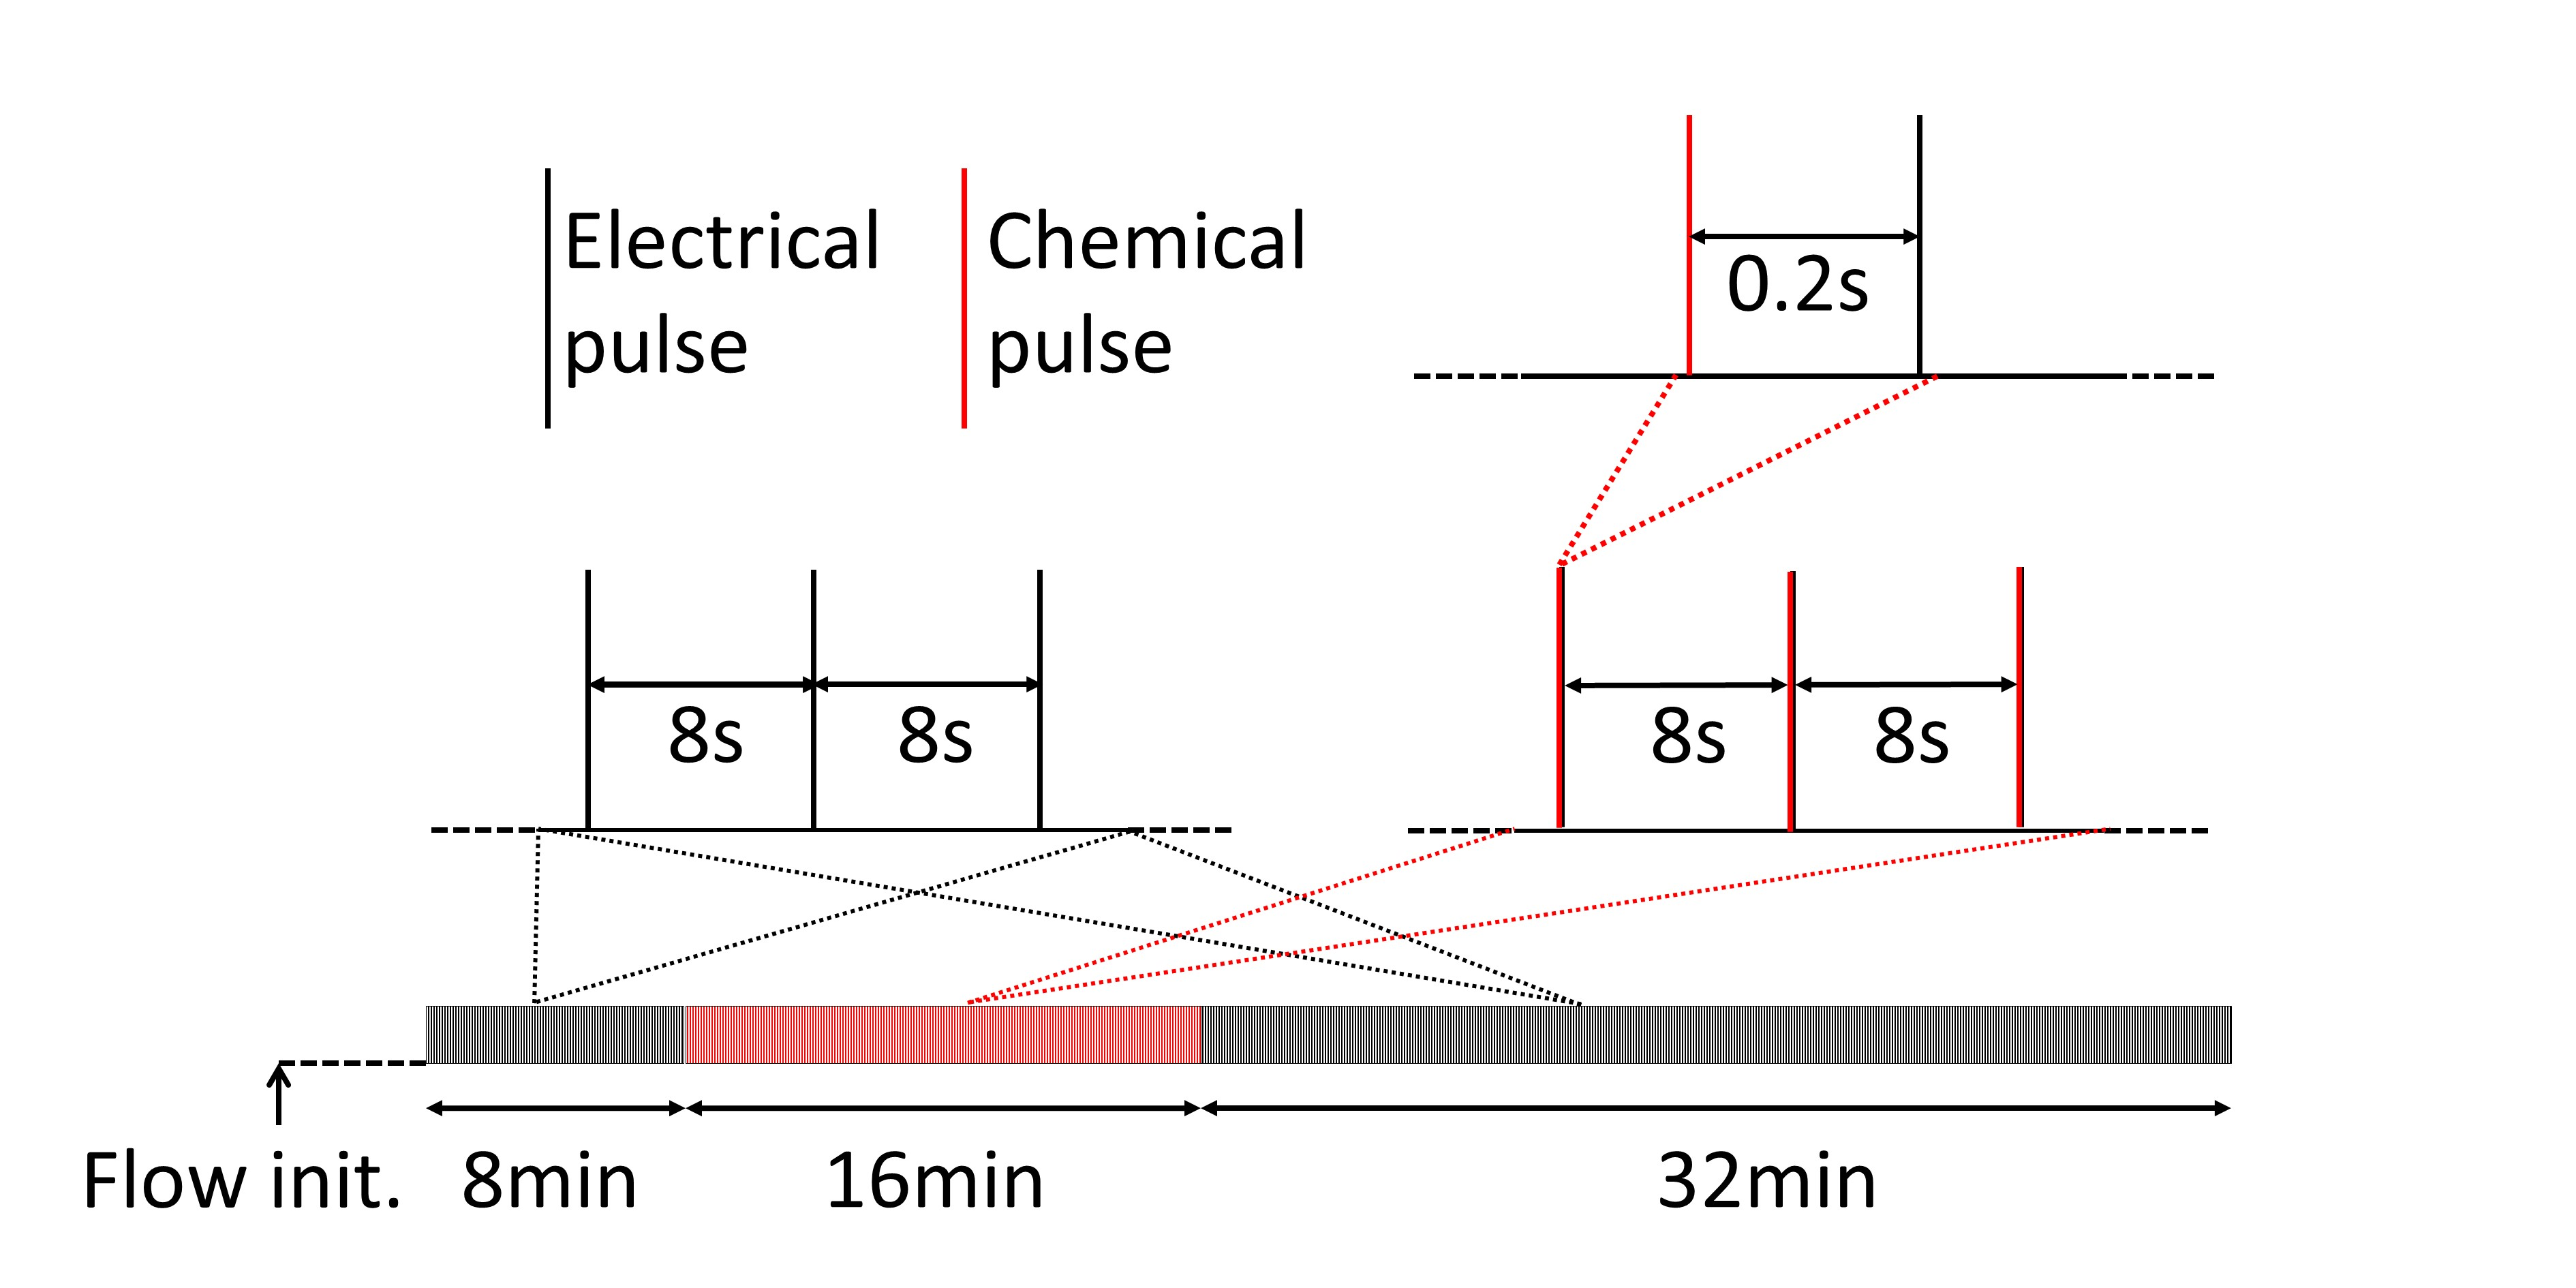
\includegraphics[width=15cm]{chapter6/figures/ExpOutline/dopamineExpOutline1.jpg}
       \caption[Illustration of the dopamine pulsing experimental protocol]{\textbf{Illustration of the dopamine pulsing experimental protocol.}}
       \label{fig:pulses:expOutline}

   \end{figure}


The pulsing commands were given \(200ms\) prior to the coupled electrical stimulations to offset the delay in arrival of the agonist. Taking into account the predicted delay in the arrival of the agonist, the pulse-stimulation timing difference meant that the cells experienced an appreciable increase in dopamine levels only after most of the stimulation-associated activity had subsided (figure \ref{fig:pulses:pulseTiming}). This precise temporal arrangement has been purposefully selected to make this experimental protocol relevant to the notion of distal reward, as explained next. Distal reward, as reviewed in section \ref{sec:introduction:neuromodulators} refers to the fact the dopamine transients associated with discrete rewarding events arrive in delay compared to the neuronal activity that was responsible for the attainment of the reward. To link the dopamine transient to the preceding neuronal activity, it was suggested that active synapses become tagged with an `eligibility trace' which decays at a time scale of several seconds \cite{izhikevich2007solving}. A synapse will be reinforced only if the dopamine transient arrives before its eligibility trace has completely decayed. Recently, such an `eligibility' time window has been demonstrated for plasticity of synaptic spines in the striatum \cite{yagishita2014critical}. Thus, the experimental paradigm employed here is designed to directly test these ideas in the culture context. Beyond its established interaction with neuronal plasticity, dopamine is also known to directly and immediately modulate neuronal circuits upon exposure \cite{gorelova2002mechanisms,ferron1984inhibitory,rodgers2011tonic,gonzalez2001dopamine,tye2013dopamine}. This effect has been linked to the generation of reward-driven behaviour \cite{bromberg2010dopamine,tye2013dopamine}. Thus the delayed administration of the agonist also aims to test whether these two separate roles of dopamine, delayed reward plasticity and direct activity modulation, can be decoupled from each other. This experimental design highlights the utility of the system in studying rapid volume transmission processes with a high level of temporal control and in a concentration-resolved manner.

 \begin{figure}[h]

      \centering
      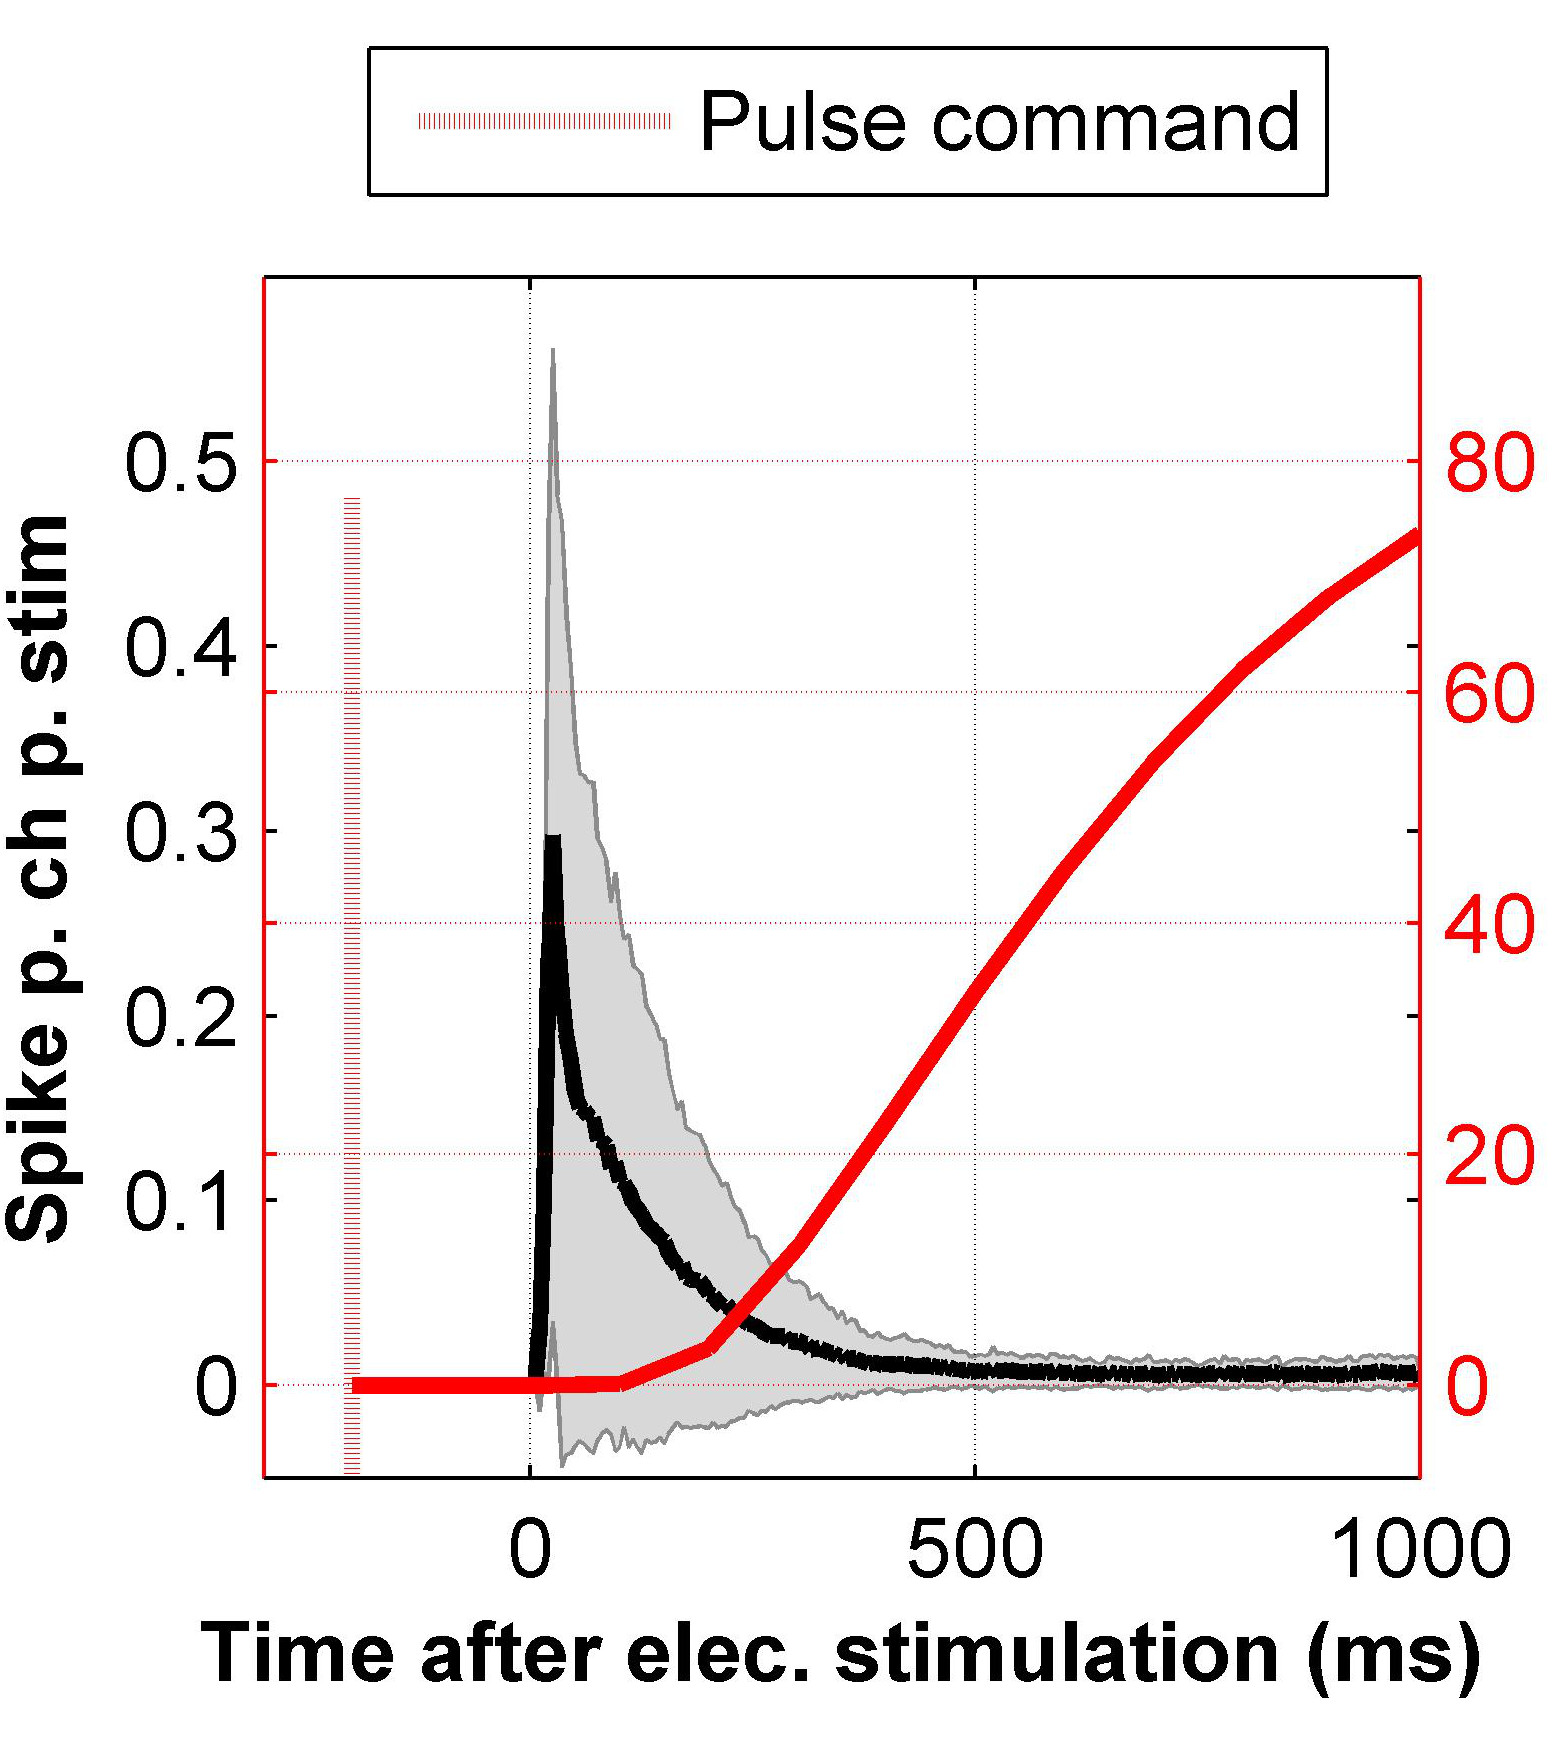
\includegraphics[width=6.6cm]{chapter6/figures/pulseTiming/dopaminePulsingPulseTiming.jpg}
      \caption[Timing of dopamine transient relative to reverberative stimulation response]{\textbf{The dopamine levels were programmed to increase only after the the reverberative stimulation response had mostly subsided.} Overlay of the predicted dopamine transient and the averaged PSTH across all pulsing experiments (n=13). Shaded area shows the PSTH standard deviation. Pulse command was given \(200 ms\) prior to the associated electrical stimulation. The timing of the dopamine transient was purposefully selected to model a `distal reward' scenario.}
      \label{fig:pulses:pulseTiming}

\end{figure}




   Figure \ref{fig:pulses:pulsingExample} shows full response rasters (averaged over all channels) of two example experiments, one with dopamine and one with buffer-only control. The stimulation responses that were coupled to dopamine pulses (marked by the red bar) were depressed (i.e., smaller in length and intensity) as compared to those induced before and after the coupling. The control data show that this depression is not a result of the pulse action itself (i.e., the sweeping of the interface across the microculture) as the responses persisted seamlessly through the pulsing epoch.

   \begin{figure}[h]
       \centering
       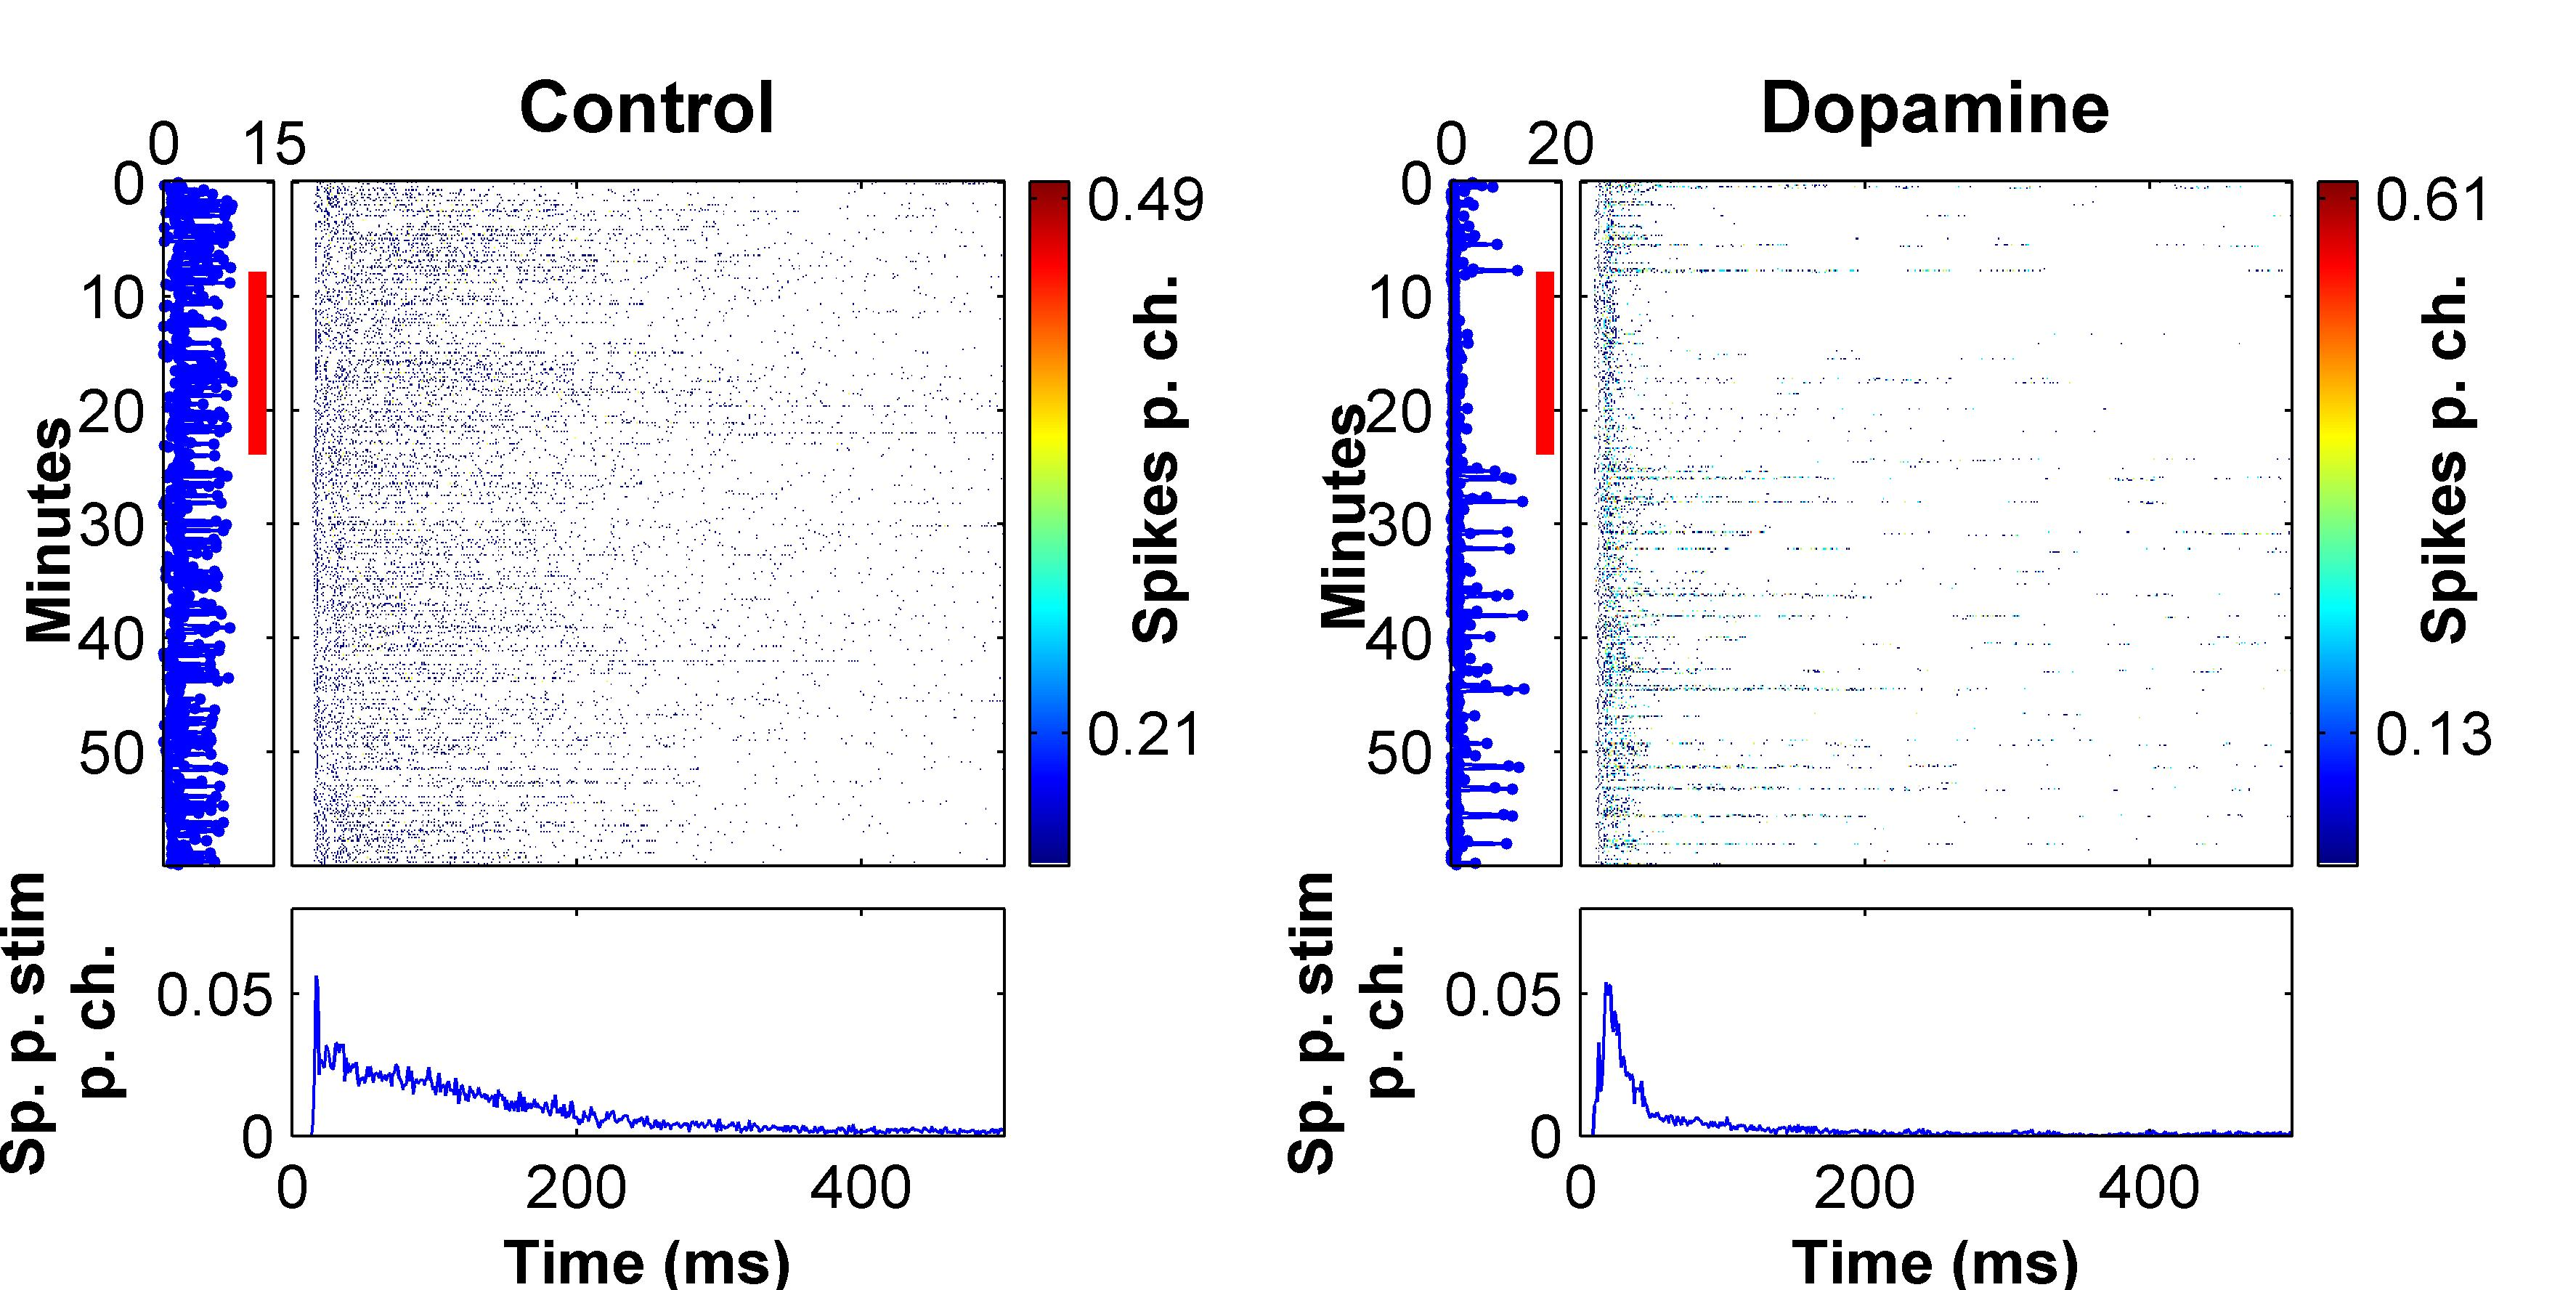
\includegraphics[width=15cm]{chapter6/figures/pulsingRasterExample/experimentRasterExample.jpg}
       \caption[Example response rasters from the dopamine pulsing experiment]{\textbf{Coupling electrical stimulations to dopamine pulses suppresses the responses whereas blank pulses have no effect.} Complete response rasters and PSTHs are shown from example control and dopamine pulsing experiments. The experimental epoch where the stimulations were coupled to dopamine are marked by red bars in the response sum panels (on the left of response rasters). Raster plots use \(1ms\) bins.}
       \label{fig:pulses:pulsingExample}

   \end{figure}
    Many of the experiments exhibited a marked increase or decrease in the intensity of the responses as the experiments progressed. However, these changes were observed both for the dopamine and control conditions. Figures \ref{fig:pulses:pulsingChannelsExampleIncrease} and \ref{fig:pulses:pulsingChannelsExampleDecrease} show such response changes broken down into the constituent channels (i.e., channel-resolved response rasters and stimulation maps). These data show that changes in the total stimulation response intensity were expressed as a general inhibition or excitation across all channels while maintaining their individual roles within the network, i.e., individual channels maintained their response latencies and their proportional firing rate. Thus, as far as this analysis can tell, the noted changes to the response intensity reflect a general drift in the excitability of the microculture rather than a change in the functional organization. In chapter \ref{chap:activityAndFlow} we argued that the fast flow interferes with intrinsic volume transmission processes within the tissue because it effectively imposes a particular concentration for the extracellular species (their concentration in the flow media). Part of the role of the extracellular environment is to dynamically respond to changes in the global activity to maintain homeostatic control and the loss of this control is likely to be responsible for the observed drift. Nevertheless, the sustainment of the functional identity of the circuit shows that the conclusions of chapter \ref{chap:activityAndFlow} are valid for the microcultures as well, i.e., that useful experimentation can be performed under these flow conditions. In practical terms, the excitability drift is reflected in the variability of experimental data and this can be seen in figure \ref{fig:pulses:FCStats} where the variability of the overall firing rate increases over experiment time.

  \begin{figure}[!htb]
       \centering
       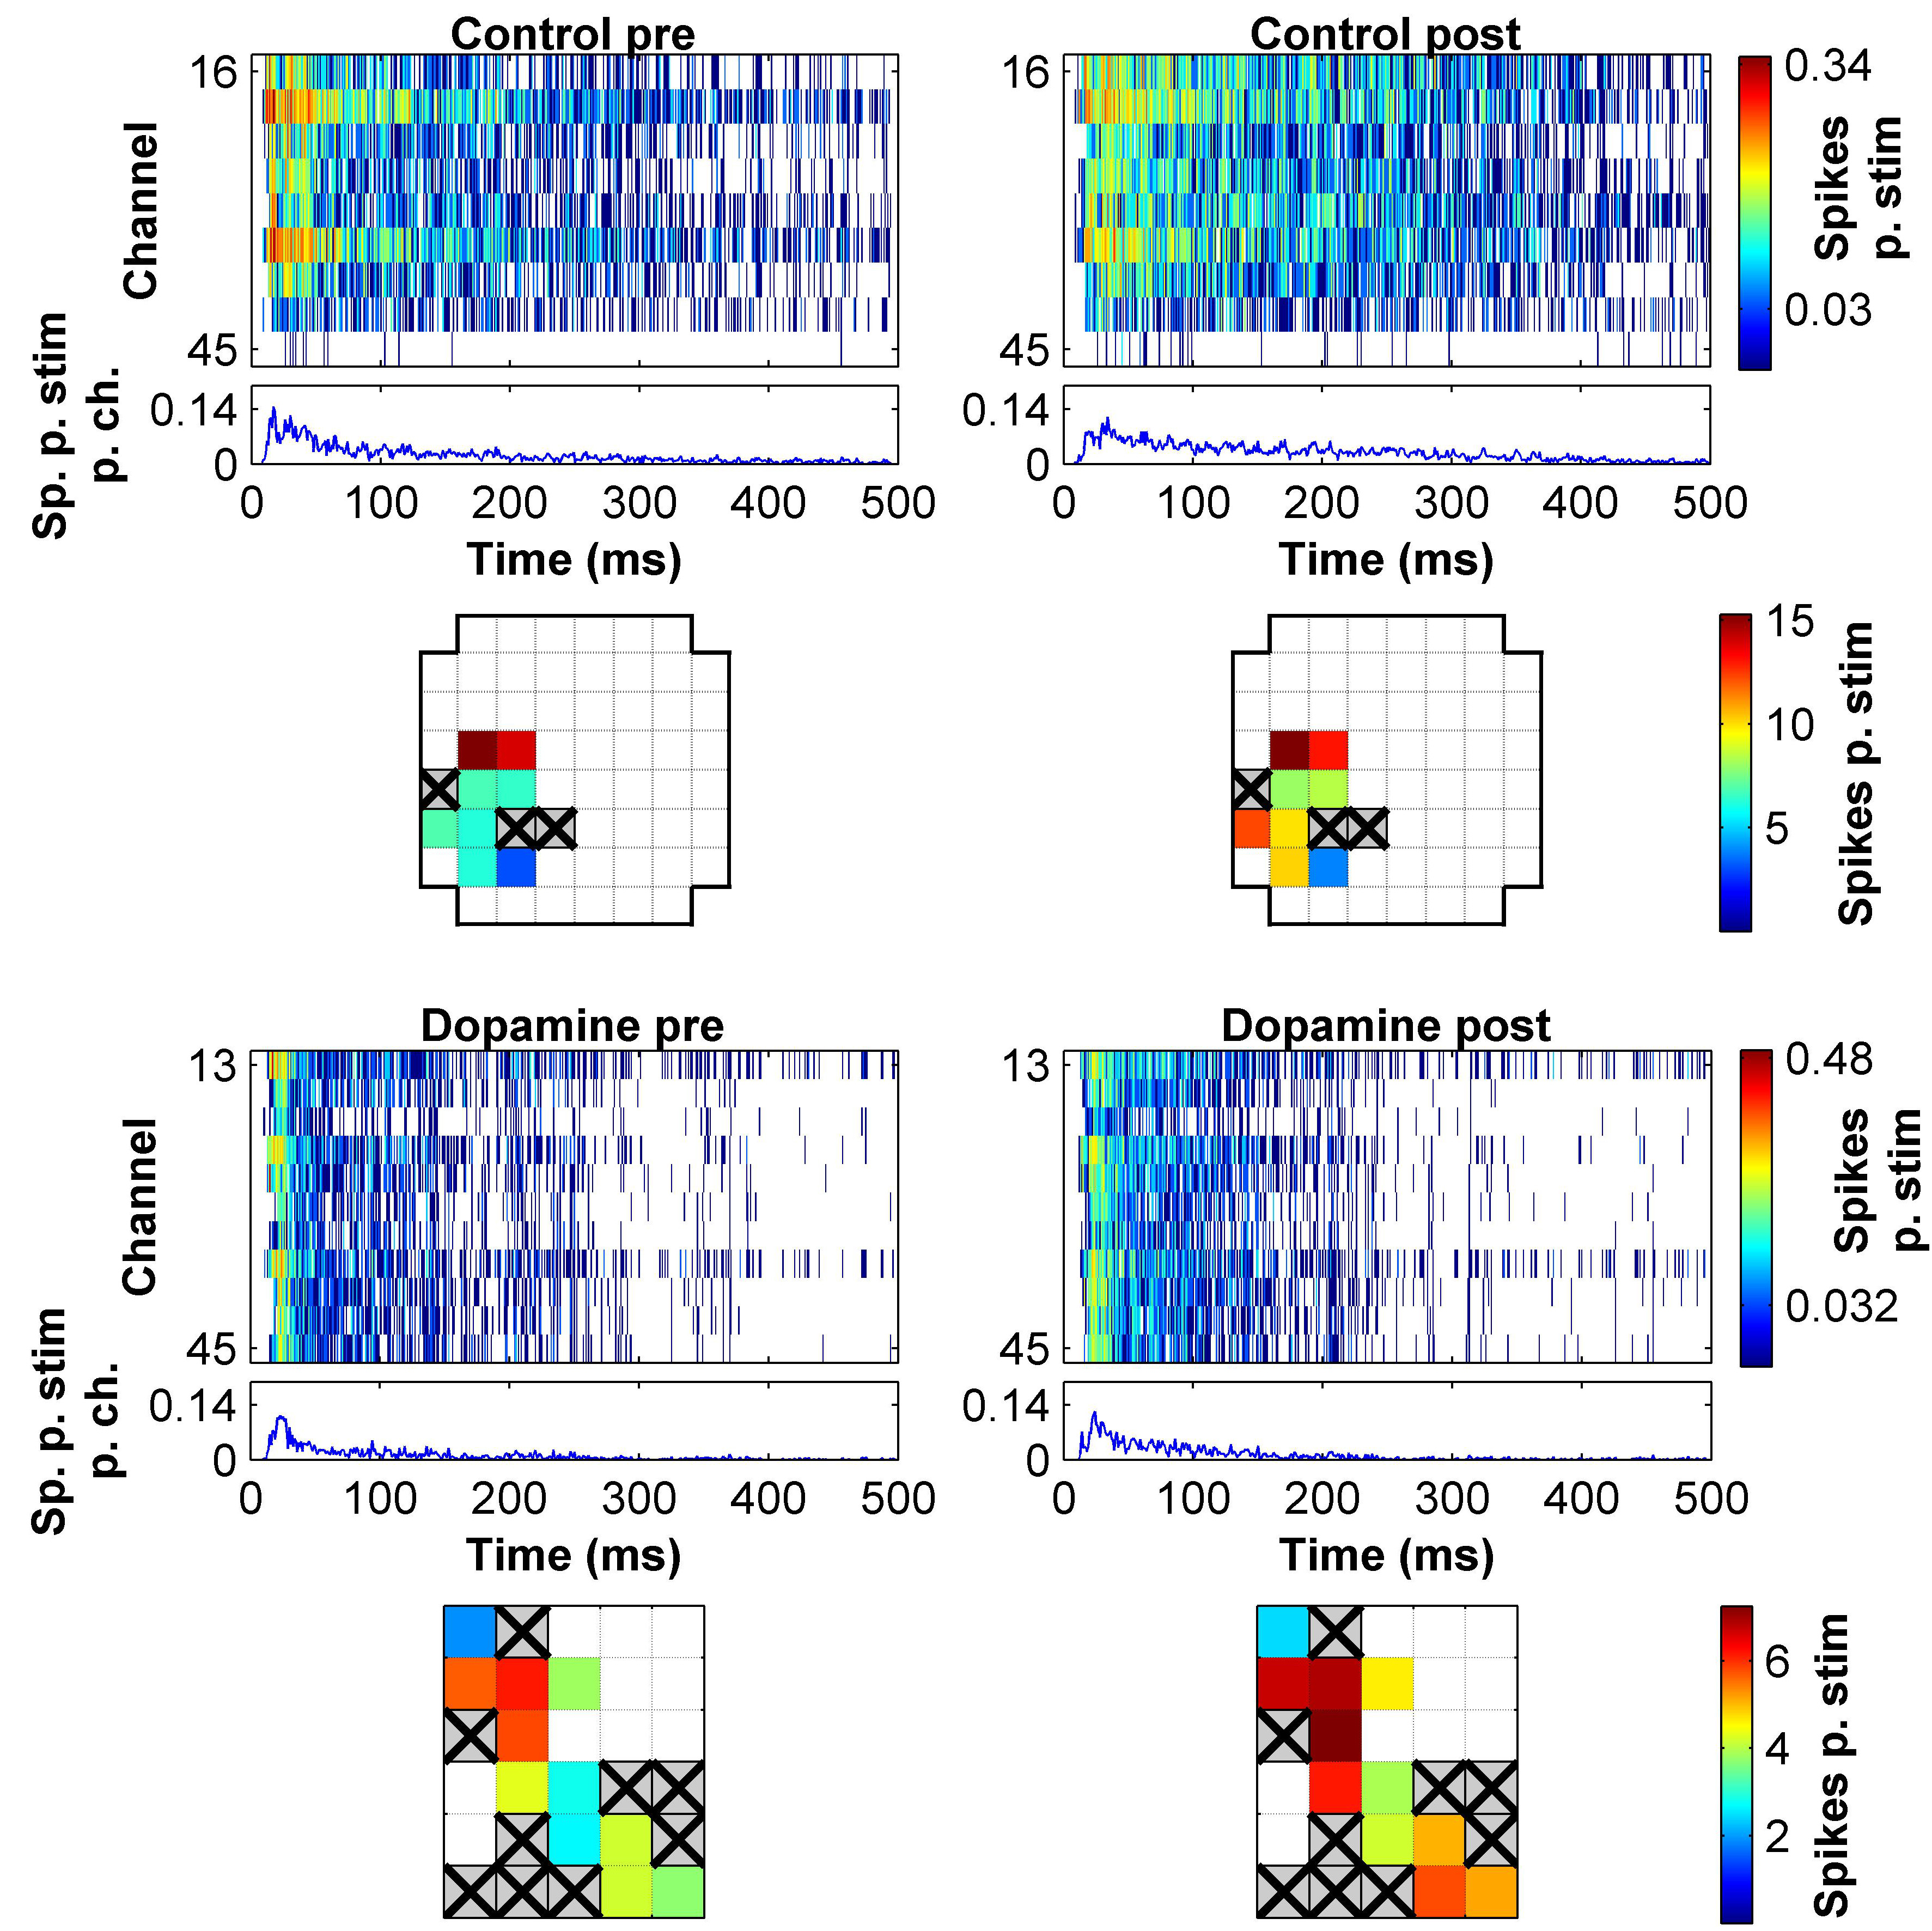
\includegraphics[width=15cm]{chapter6/figures/pulsingChannelsExample/pulsesChannelExampleIncrease.jpg}

       \caption[Channel PSTHs before and after administration of pulsing protocol with dopamine or control solutions - example of global increase in response intensity]{\textbf{Some of the dopamine and control experiments exhibited an increase in response intensity following the pulsing but without reorganization of relative channel firing rates.} Comparison of channel PSTHs and stimulation response maps before and after the pulsing epoch in example control and dopamine experiments. Each of the data sets is based on an 8 minute recording bins. The pre bin refers to the experimental segment prior to the pulsing. The post block refers to the second bin after the termination of the pulsing. These specific data are examples of increases in the global response intensity. The response rasters and particularly the summated PSTHs (panels directly below the channel rasters) show that the difference is mainly associated with a lengthening of the reverberative stimulation response. Stimulating electrodes are marked with X. The control data were collected from a device assembled on a \(8\times8\) MEA. Thus the graphic stimulation response maps show the relative location of the microculture on the electrode grid. The dopamine data were collected on a HDMEA in which case a single \(5\times6\) block is shown.}

       \label{fig:pulses:pulsingChannelsExampleIncrease}
  \end{figure}

  \begin{figure}[!htb]
       \centering
       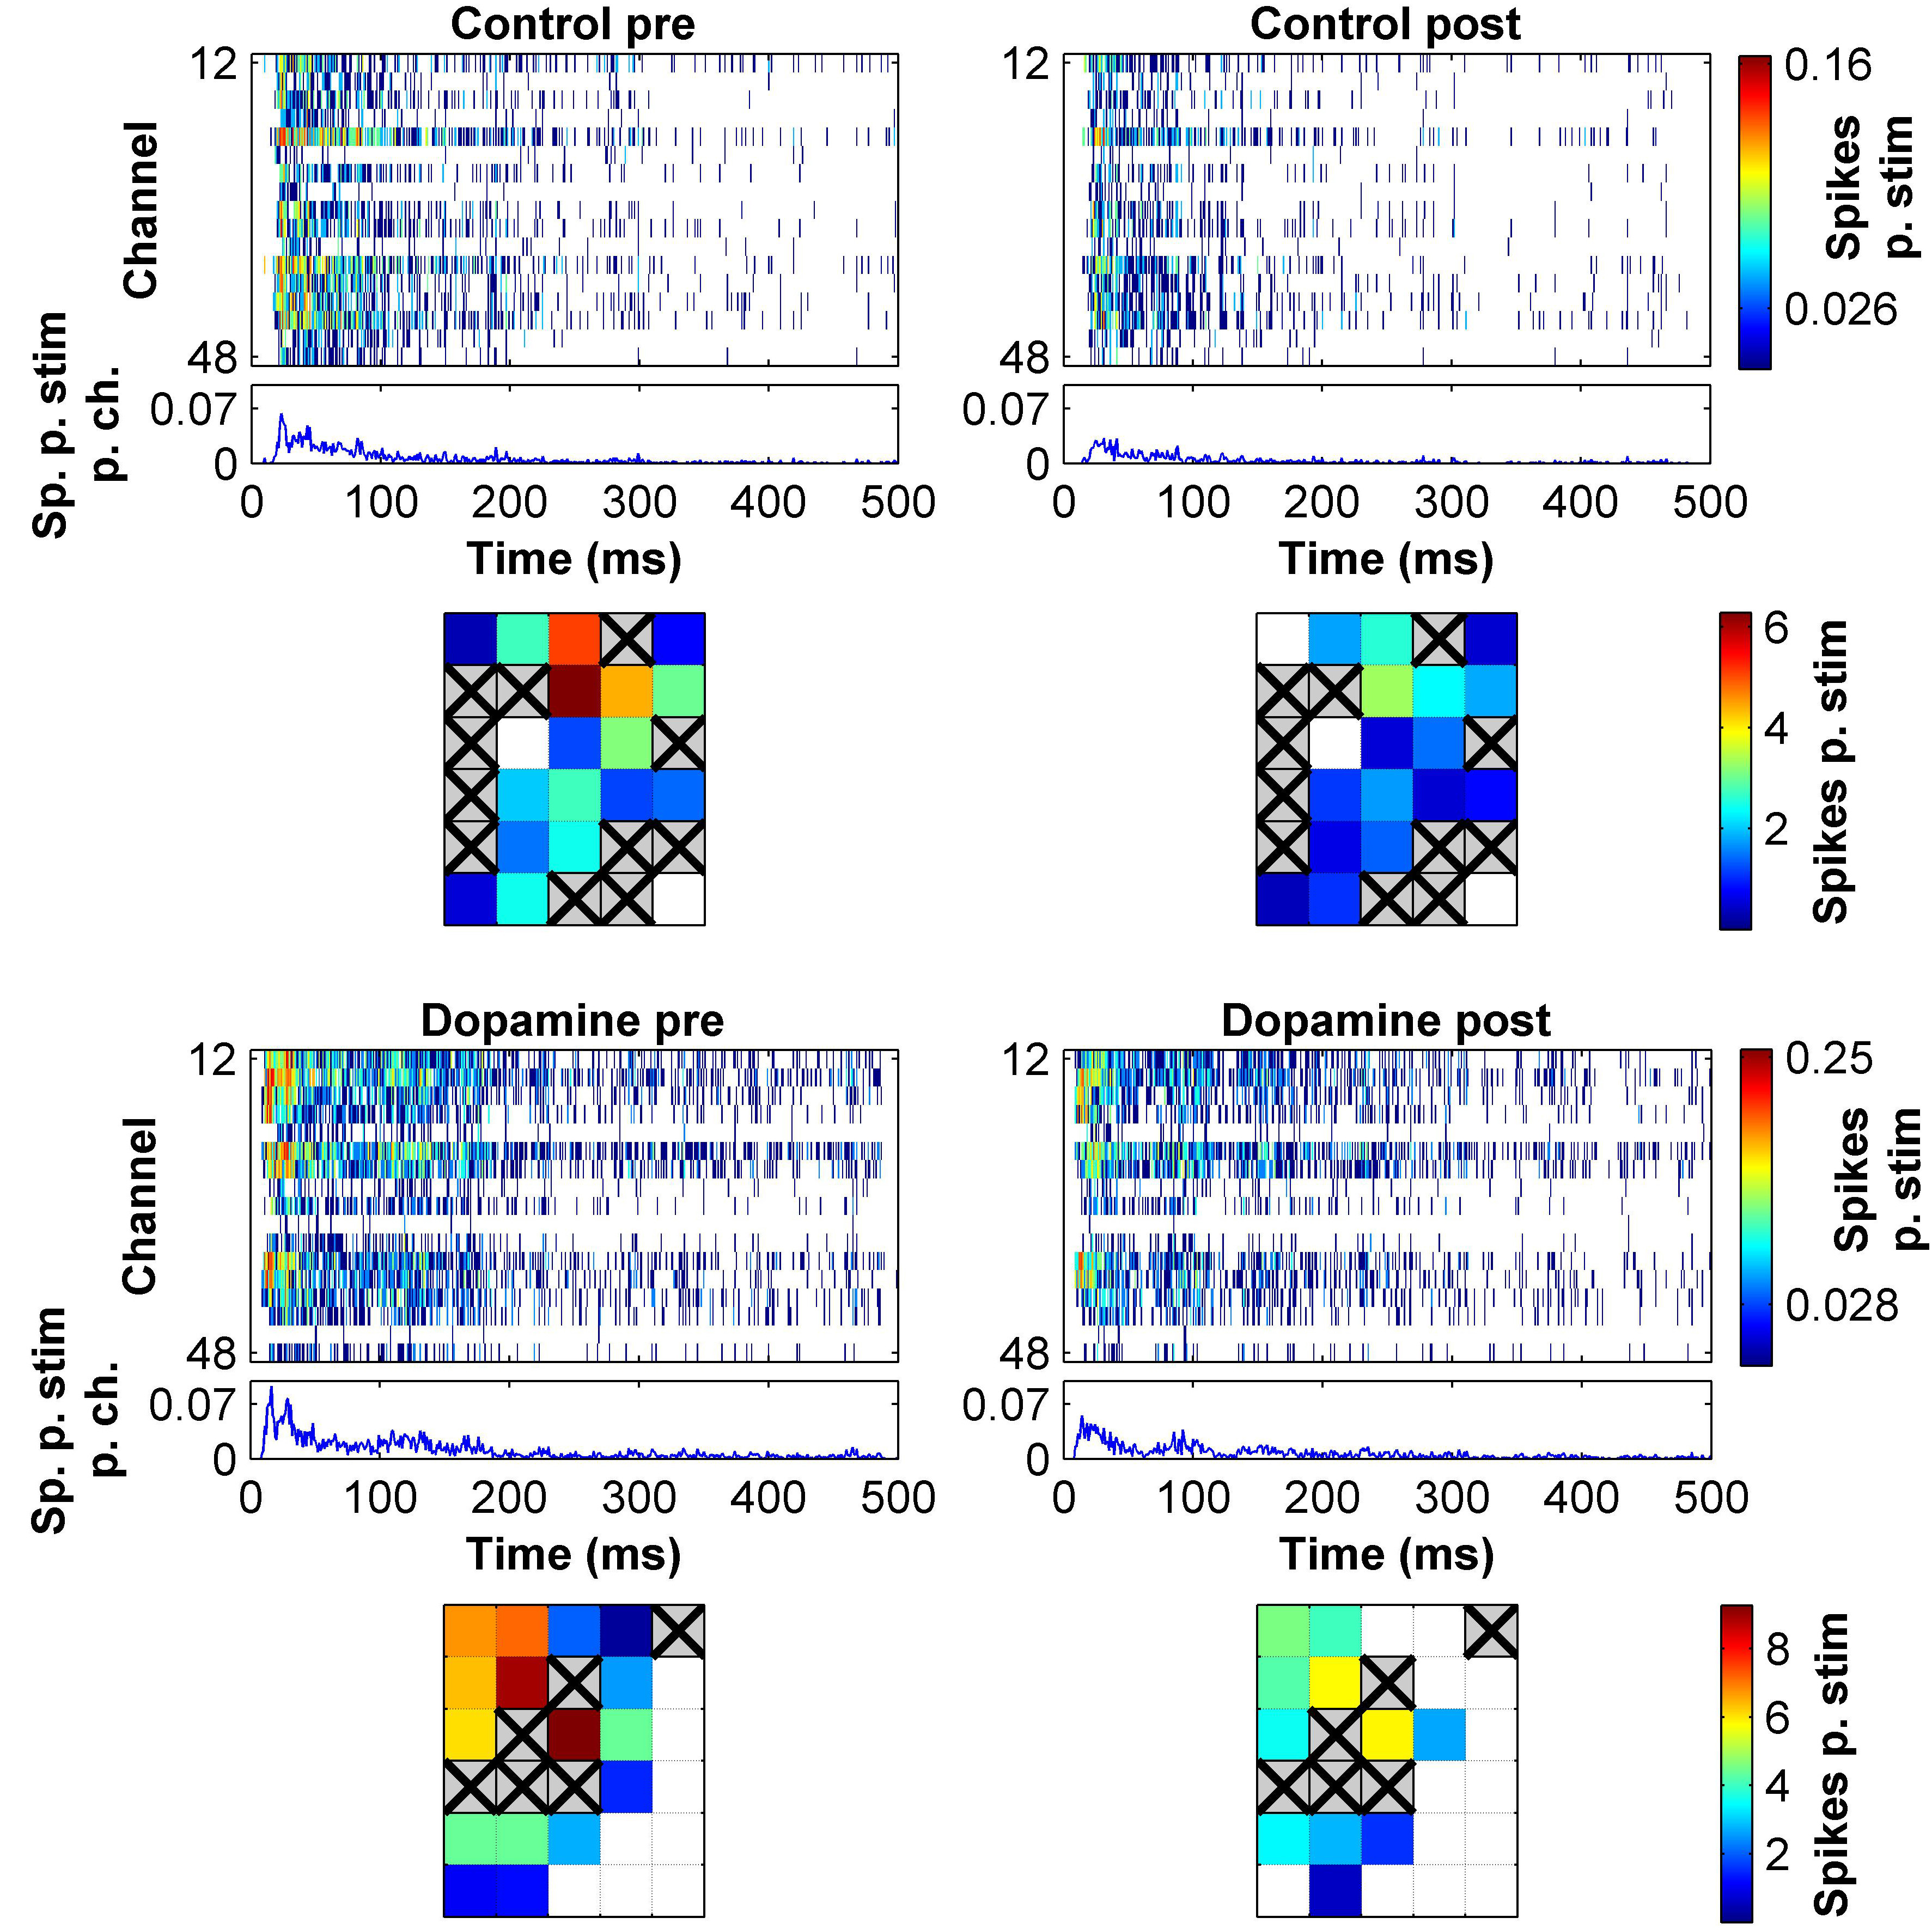
\includegraphics[width=15cm]{chapter6/figures/pulsingChannelsExample/pulsesChannelExampleDecrease.jpg}

       \caption[Channel PSTHs before and after administration of pulsing protocol with dopamine or control solutions - example of global decrease in response intensity]{\textbf{Some of the dopamine and control experiments exhibited a decrease in response intensity following the pulsing but without reorganization of relative channel firing rates.} Comparison of channel PSTHs and stimulation response maps before and after the pulsing epoch in example control and dopamine experiments as in figure \ref{fig:pulses:pulsingChannelsExampleIncrease}. These specific data are examples of decreases in the global response intensity. The response rasters and the summated PSTHs (panels directly below the channel rasters) suggest that the difference is associated with a decrease in initial firing rates of the reverberative stimulation response as well as with a shortening in its length.}

       \label{fig:pulses:pulsingChannelsExampleDecrease}
  \end{figure}



  To provide an improved grounds for interpreting the results of the experiments we estimated the the degree of receptor activation during the dopamine transients using the Michaelis-Menten equation. This approach requires a value for the affinity (dissociation constant) of the dopamine receptors. However, the literature provides contradictory affinity values. In part, this has to do with these receptors having been shown to exist in two states with several orders of magnitude difference in affinities when expressed \textit{in vitro} making it unclear which state they take on \textit{in vivo} \cite{seeman1994dopamine,richfield1989anatomical}. At the same time, direct \textit{in vivo} measurement of the affinity using radioligands is problematic due to nonspecific interactions in the native tissue \cite{seeman1980brain}. Nevertheless, Radioligand studies in intact tissue slices showed that both D1 and D2 receptor appear in rat brain in a mix of high affinity and and low affinity states \cite{richfield1989anatomical}. This suggests that they occur in different brain regions in different affinity states and have the ability to switch between them. The factors which determine such switching remain unknown, though. Given these complications, it is unsurprising that reported affinity values have varied between \(K_{d}=1-3000 nM\). Most of the reports in rats, though, seem to have been clustered at values of \(K_{d}=1-20 nM\) for both main receptor subtypes \cite{seeman1980brain}. Such low values, however, seem inconsistent with the amperometric accounts of dopamine concentration \textit{in vivo}. Such reports have indicated that, in the striatum, dopamine levels fluctuate between \(30nM\) at baseline and \(100-200nM\) at the peak of phasic transients \cite{venton2003real,brown2011primary,phillips2003subsecond}. If dopamine levels already exceed the dissociation constant at baseline it would leave little dynamic range for phasic transients to have an impact. Given these arguments, we finally estimated the receptor activation using a dissociation constant of \(K_{d}=100 nM\) which seems plausible given both the radioligand and the amperometric reports. However, this very rough estimation is used solely to give an impression rather than to draw quantitative conclusions. In this study we used a dopamine concentration of \(100 \mu M\) in the agonist stream which is the standard level used for inducing maximal activation of dopamine receptors \cite{seeman1980brain} and is the typical concentration applied in bath application experiments (e.g., \cite{eytan2004dopamine,yagishita2014critical}). However, because this concentration is 3 orders of magnitude higher than the speculated dissociation constant, the effective activation of the dopamine receptors is much wider than is apparent from the concentration transients (figure \ref{fig:pulses:receptorSat} B). Alas, this information depends on a speculative value for \(K_{d}\) but even the lowest reported value is still 2 orders of magnitude lower than the agonist stream concentration. Consequently, it should be taken into account that the effective separation between consecutive activations of the dopamine machinery is probably less than a second as shown in the figure.

  \begin{figure}[h]
       \centering
       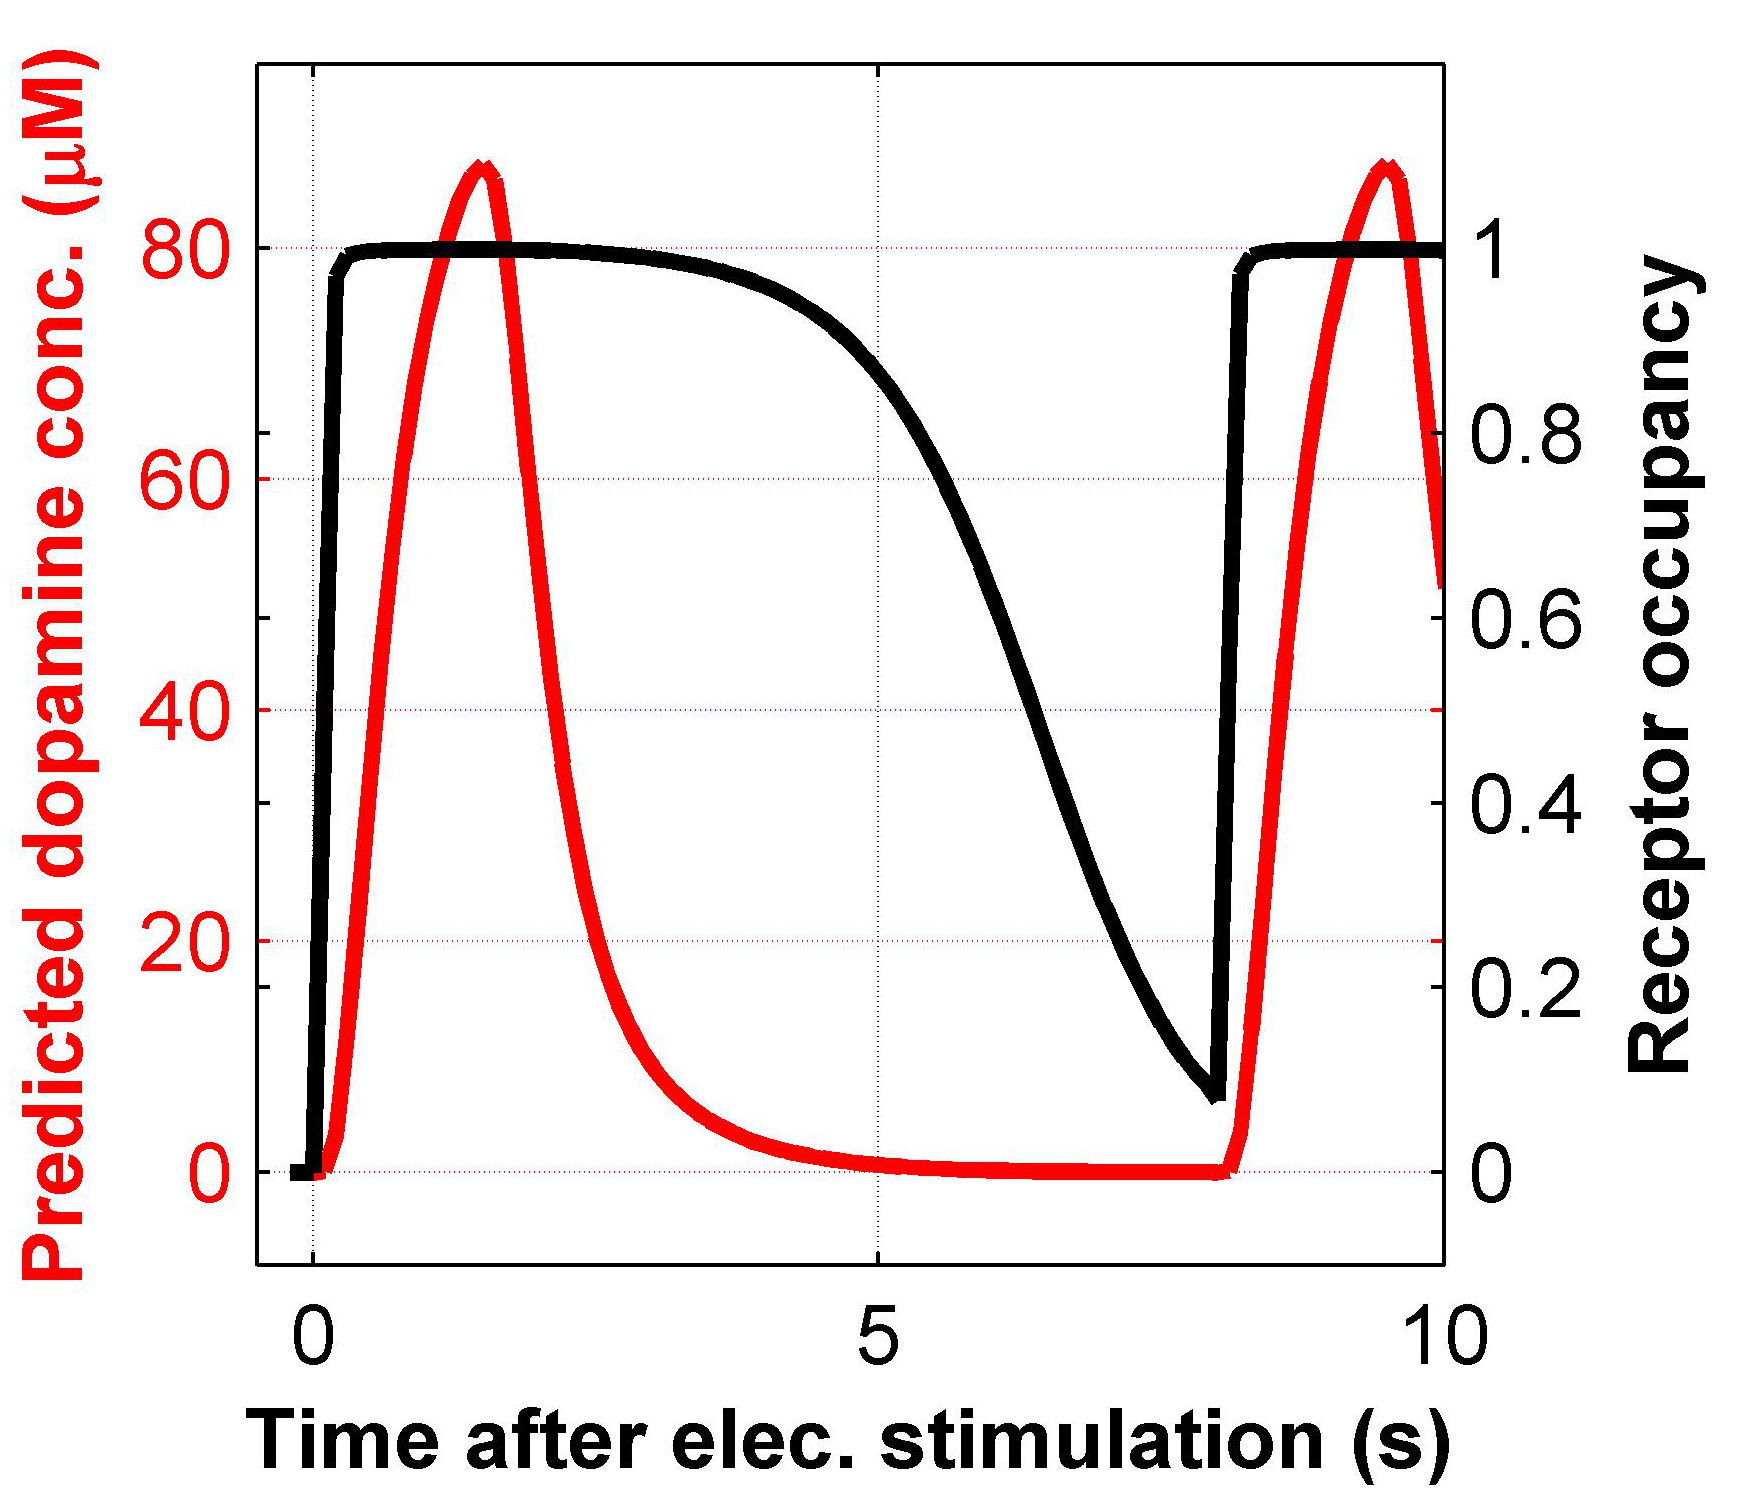
\includegraphics[width=7cm]{chapter6/figures/receptorSat/dopaminePulsingReceptorSat.jpg}

        \caption[Estimated dopamine receptor occupancy levels during a dopamine transient]{\textbf{Due to the orders of magnitude discrepancy between the dopamine concentration in the agonist stream and the dopamine receptor dissociation constant, consecutive receptor activations were probably less temporally separate than apparent from the dopamine time course.} Estimated dopamine receptors activation (black curve) over an entire dopamine transient (red curve) cycle. Receptor activation was estimated using standard Michaelis-Menten equilibrium and an approximate dissociation constant of \(100nM\). See text for further information about this estimation. Dopamine concentration in the input stream was \(100\mu M\). Dopamine pulsing experiments were performed in devices with \(80\mu m\) deep microwells.}

       \label{fig:pulses:receptorSat}

  \end{figure}

  Despite the programmed delay in the the arrival of the dopamine transient relative to the electrical stimulation, the spiking responses became depressed for the period of time that they were coupled to dopamine pulses (figure \ref{fig:pulses:FCStats} A, unbalanced t-test, \(p=0.025\) and \(0.028\) for the two bins spanning the pulsing epoch) and reverted back to baseline soon after the pulsing was concluded. Such a temporary effect is indicative of a direct influence of the dopamine on the network dynamics rather than of synaptic plasticity. This suggests that the effect of dopamine persisted beyond the physical presence of the agonist and that the pulse configuration used here did not give enough time between transients to allow recovery. These results demonstrate that dopamine neuromodulation is functional in these microcultures and align well with the known direct effect of neuromodulatory system on cortical dynamics (see section \ref{sec:introduction:neuromodulators}).

    \begin{figure}[!htb]
       \centering
       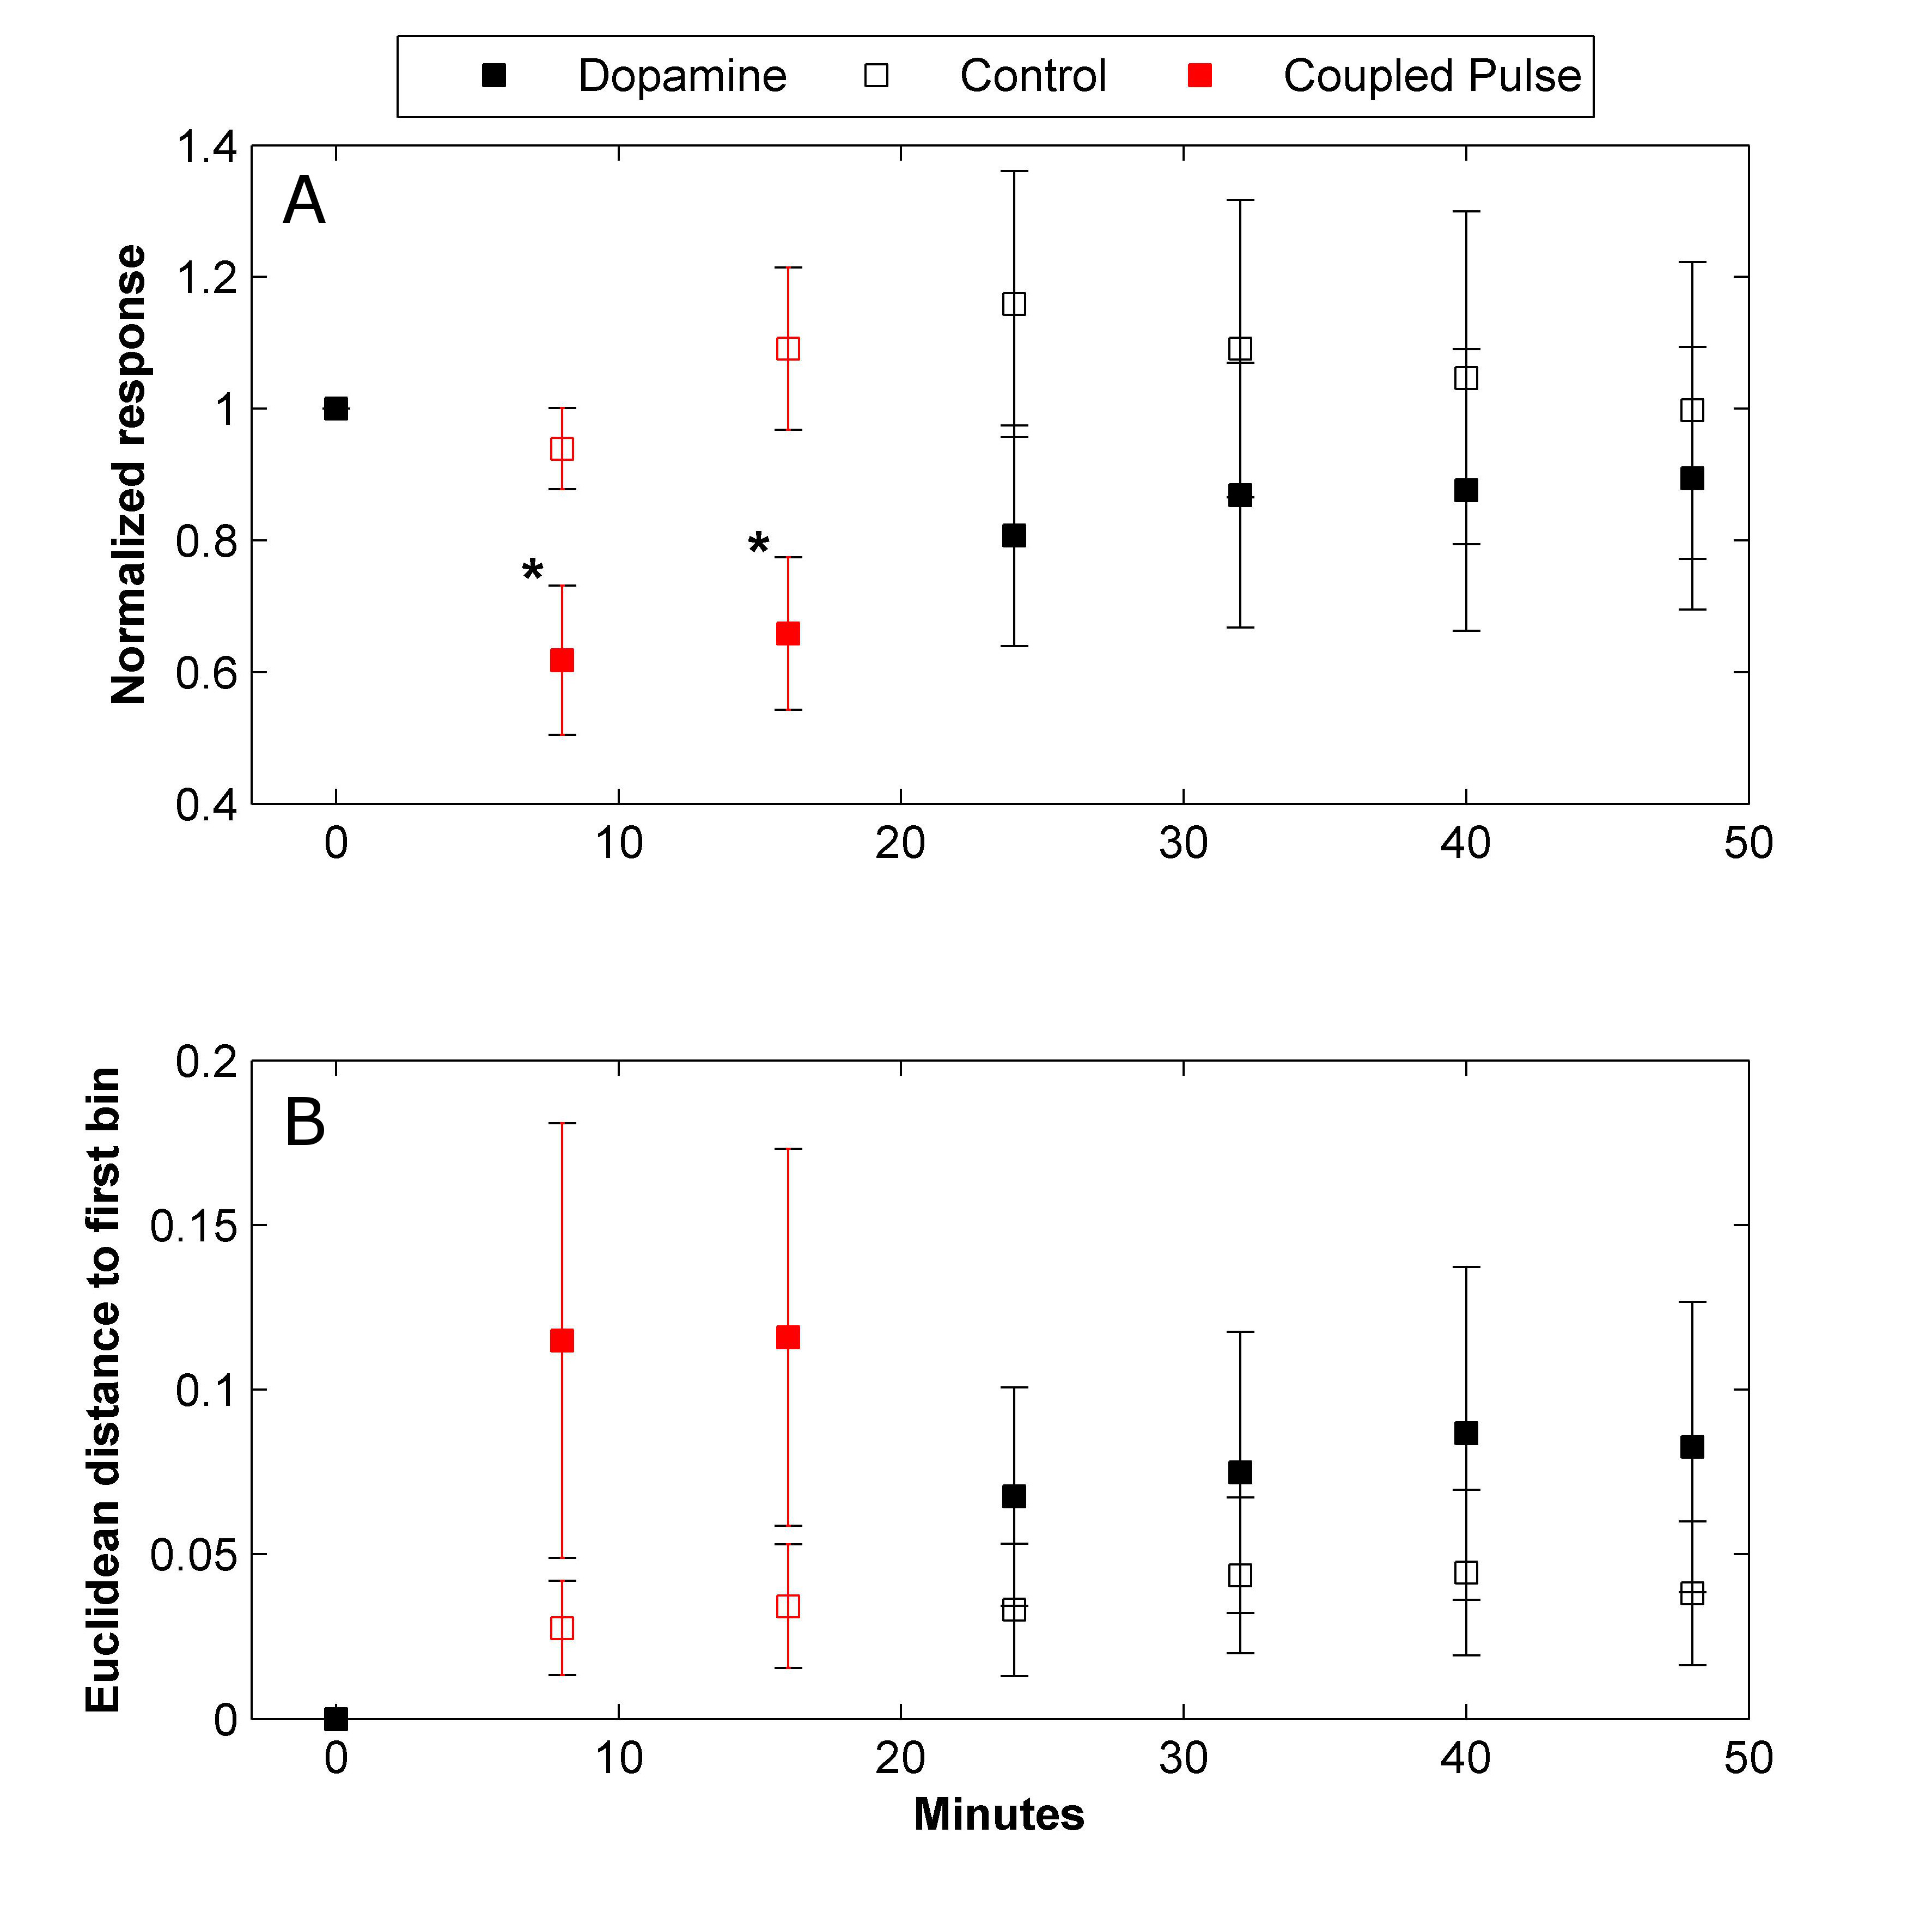
\includegraphics[width=15cm]{chapter6/figures/FCStats/FCStats.jpg}
        \caption[Global stimulation response and functional connectivity analysis of the dopamine pulsing experiments]{\textbf{Association of the electrical stimulation with dopamine pulses causes a temporary inhibition of evoked responses.} (A) Comparison of the time course of global stimulation responses between experimental conditions of dopamine (n=6) and blank (n=7) pulsing. Stimulation responses are averaged over all channels and all experiments in 8 minute bins. Red squares indicate bins where the electrical stimulations were coupled to dopamine pulsing. Responses are normalized to the baseline epoch (i.e,. the block preceding the pulsing) in each experiment. Error bars show SEM. (B) Functional connectivity analysis where the measure is computed over 8 minute bins of activity and presented as in A. Asterisk indicates a statistically significant difference between control and dopamine at the given block at a 95\% level of confidence.}
       \label{fig:pulses:FCStats}

  \end{figure}


  Since synaptic plasticity was not observed in the above-described measure of global response we repeated the analyses performed in section \ref{sec:activity:plasticityProtocol} and which were designed to detect changes in the detailed response distributions of the channels (figure \ref{fig:pulses:dopamineStats}) or in the functional connectivity (FC) between them (figure \ref{fig:pulses:FCStats} B). These analyses did not reveal any significant changes induced by the dopamine pulsing as compared to blank pulsing. Nevertheless, it should be noted that despite the lack of statistical significance there is a visible hysteresis in how the global response and functional connectivity measures drift back to baseline after the dopamine pulsing epoch (i.e., the time course after termination of the pulsing is visually different in the dopamine case than in the control). This might indicate that there is a certain degree of plasticity which requires a longer induction protocol to emerge as significant or that some components of the direct dopamine effect take longer to decay.

  We plan to use this system for further exploration of experimental paradigms to uncover the conditions for induction of dopamine-dependent plasticity. We believe that this system will be useful in understanding the principles behind dopamine's dual role in shaping the network dynamics and in reinforcement learning.


  \begin{figure}[!htb]
       \centering
       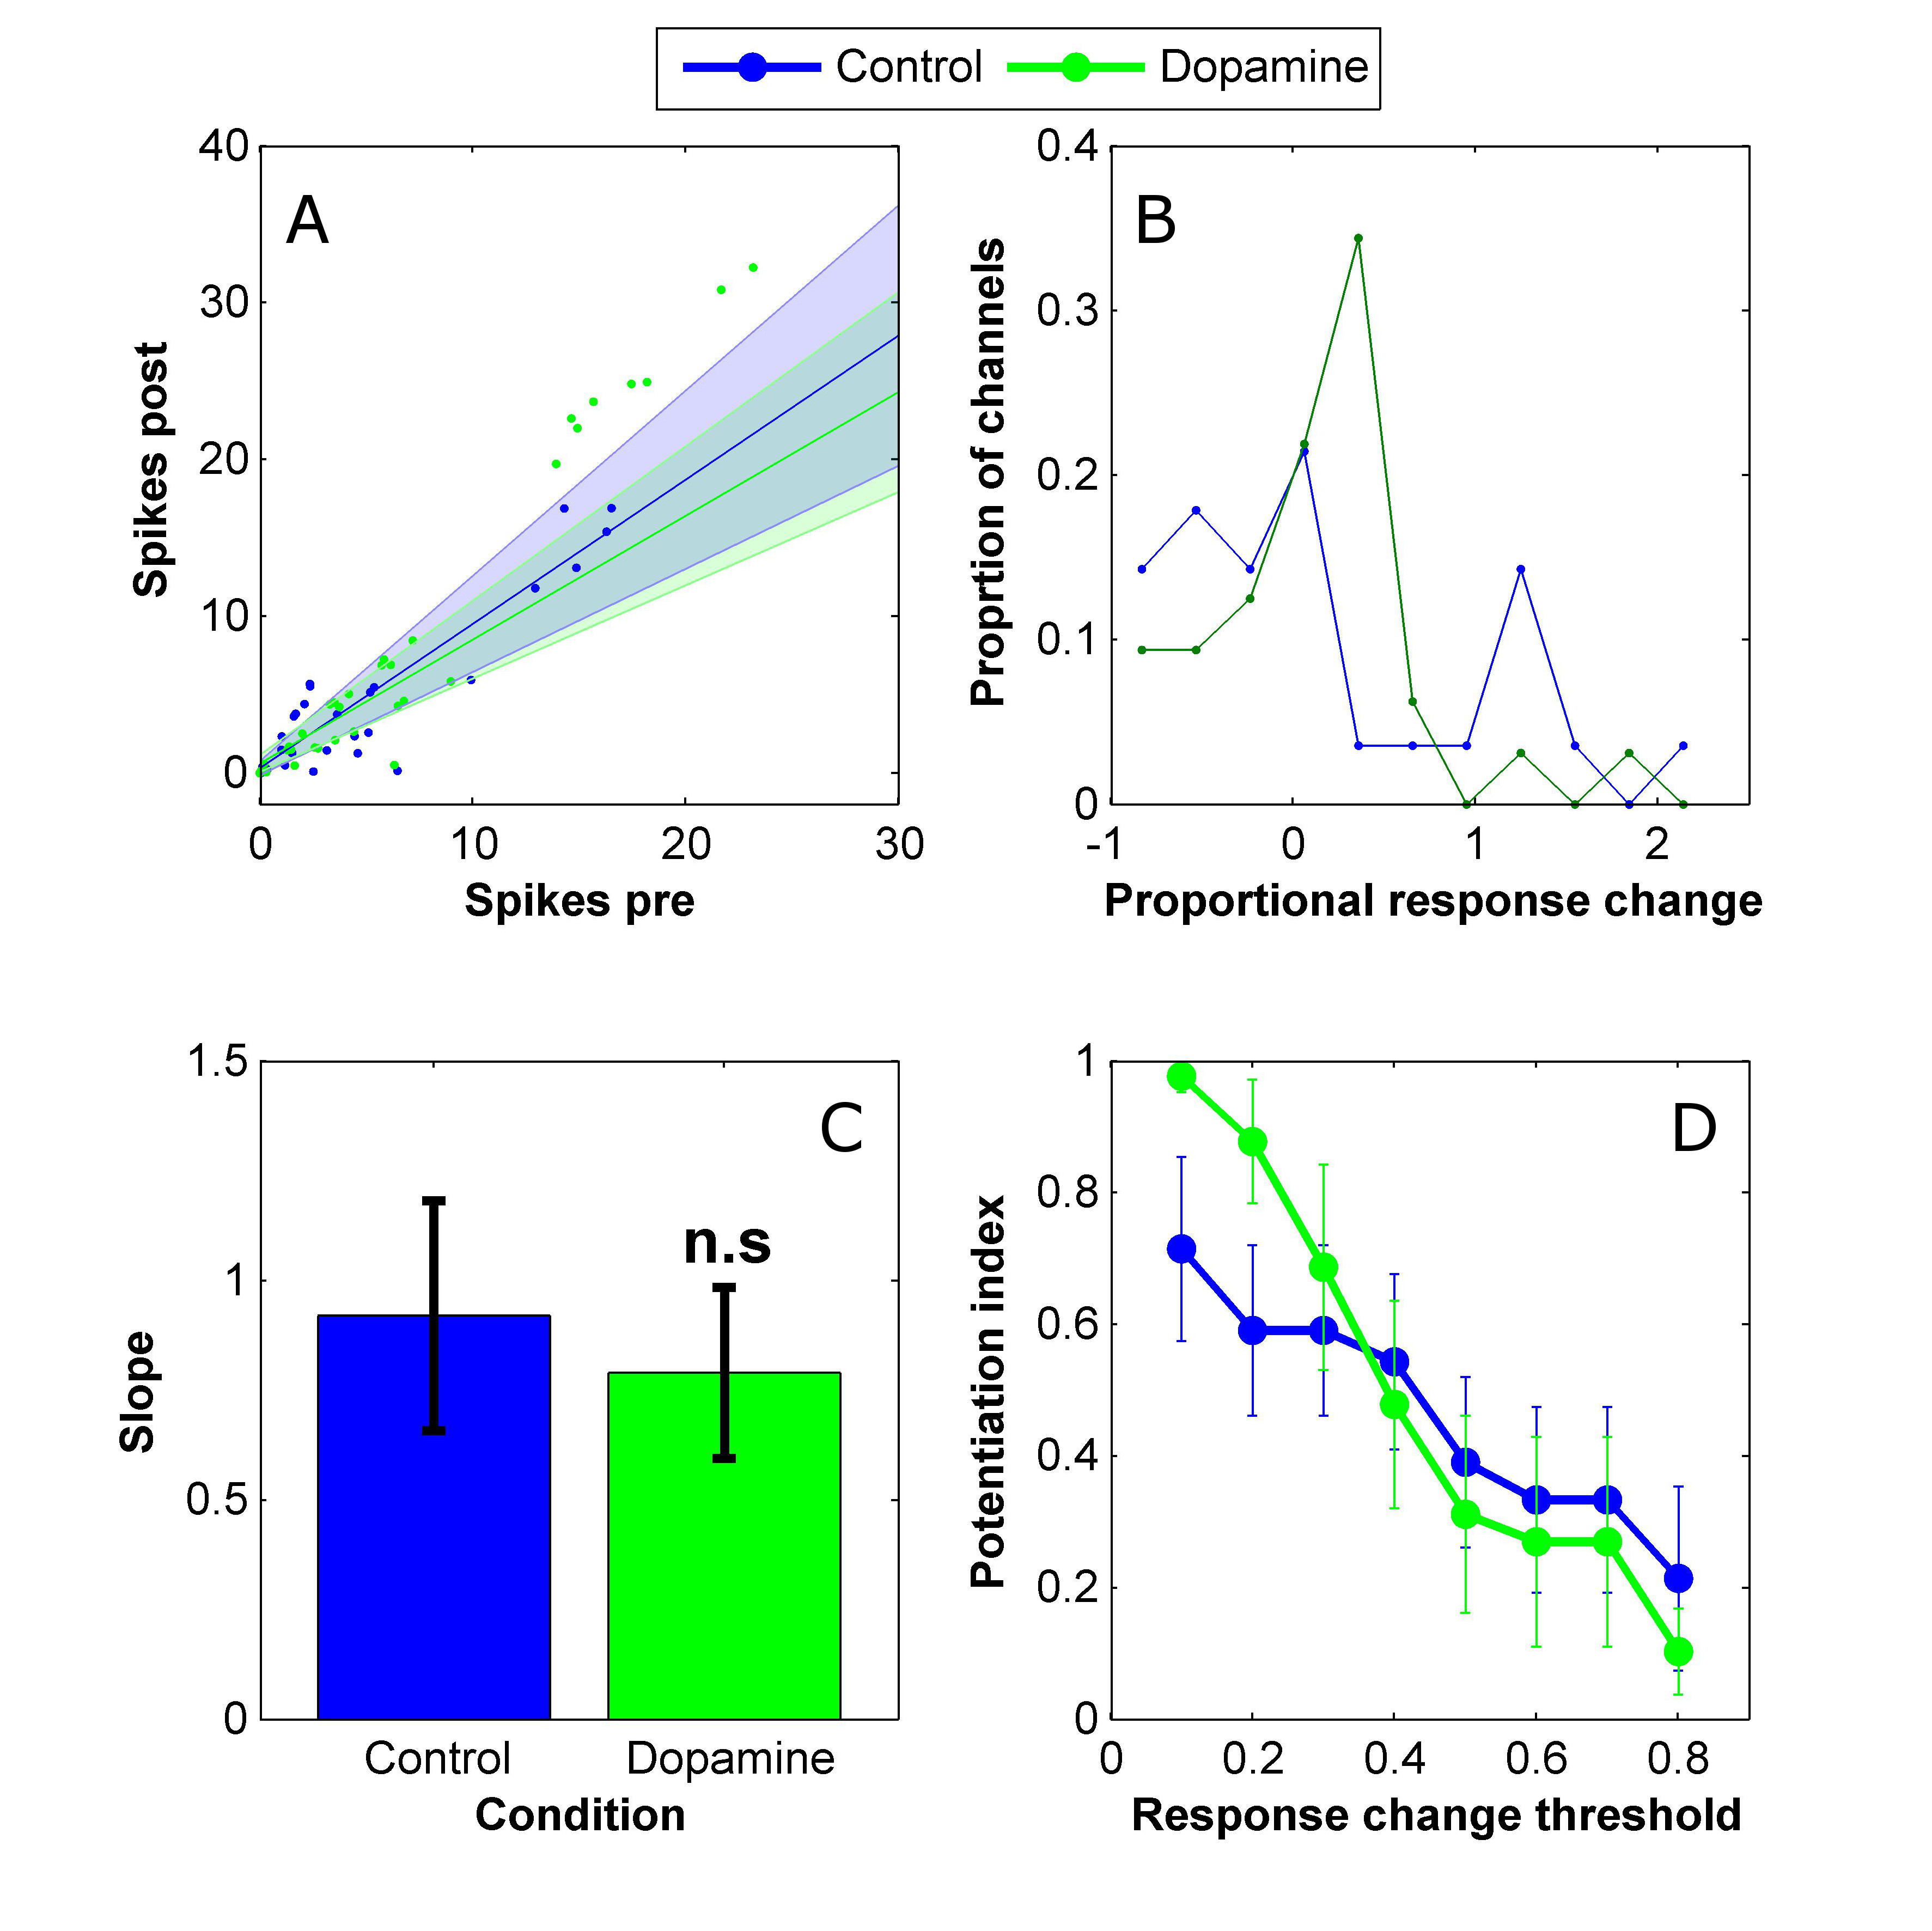
\includegraphics[width=15cm]{chapter6/figures/dopamineStats/dopamineStats.jpg}
       \caption[Statistics of the change in evoked responses following dopamine or blank pulsing]{\textbf{In this experimental configuration, coupling electrical stimulation to dopamine pulses did not elicit long term changes to global responses or a significant change in response distributions across the channels as compared to control.} The analysis in this figure completely repeats the one performed for the tetanus induction protocol in figure \ref{fig:activity:tetResChange} for comparative purposes. (A) Scatter plot of pre vs. post channel responses for the dopamine and control conditions. Pre refers to the 8 minute data bin prior to the pulsing and post refers to the second bin of such size after the pulsing has terminated. A line is fitted to the scattered points of each experimental condition. Plotted lines and shaded areas visualize the mean and SEM of these line slopes. (B) Comparison of fitted slopes from A. `n.s' - non significant difference. (C) Distributions of proportional changes induced in channel responses when compared between the pre and post epochs as in A. Potentiation index (PI) is computed based on these distributions as in figure \ref{fig:activity:tetResChange}. (D) Mean + SEM of potentiation index as a function of tested levels of change thresholds (see section \ref{sec:activity:plasticityProtocol} and figure \ref{fig:activity:tetResChange}).}
       \label{fig:pulses:dopamineStats}
  \end{figure}

In contrast to the results of section \ref{sec:activity:plasticityProtocol}, where persistent changes were observed after the plasticity induction in the presence of dopamine, no significant long lasting effects were observed with the dopamine induction performed here. The results of these two studies are not directly comparable because the induction method was different (tetanus vs. low frequency stimulation). Nevertheless, the approach followed in this chapter is superior because of its explicit control over the agonist concentration levels and because it inherently avoids artifacts associated with the solution exchange (as the culture is continuously under a steady rate of media replenishment). Thus, the contradiction in results calls for a reevaluation of the confounding factors in the previous study.

\section{Chapter conclusion}
In this chapter we put together the knowledge gathered in the previous ones to construct a system for rapid solution exchange to an entire neuronal microculture at time scales compatible with phasic neuromodulation. In spite of of the work performed in the previous chapters some uncertainties had remained uncleared, namely, whether the microcultures would be electrophysiologicaly functional, whether they would sustain that functionality under flow, whether the pulsing action would perturb the activity and whether the system can indeed match physiological time scales. These gaps have all been addressed here as we demonstrated that the microcultures exhibit spontaneous and evoked reverberative activity, that they are able to sustain that activity under flow with good efficacy, that they are oblivious to the interface shifting in itself and that the agonist transients can be applied with our current system configuration at time scales within the known range of phasic neuromodulatory signals.

We also demonstrated through simulation that faster time scales can be achieved to cover the full reported range \textit{in vivo}. Such options, however come with a caveat that they require increased flow rates. In chapters \ref{chap:devicesAndFlow} and \ref{chap:activityAndFlow} we provided data to show that, beyond a certain flow threshold, the viability and functionality of the culture are completely determined by media conditioning and are not modulated by the shear in any way. It therefore stands to reason that the results shown here apply for higher flow rates as well. Nevertheless, there will be a shear threshold which, when exceeded, will result in physical damage to the tissue and so higher flow rates would need to be tested.

We finalized the work by designing and running a plasticity experiment involving an interaction between phasic dopamine transients and stimulation induced reverberatory activity, which evoked short-term depression during co-stimulation. This experimental design highlights the usefulness of the presented system in studying how fine temporal features of phasic volume transmission interact with the activity. To our knowledge, this is the first demonstration of programmatic control over the concentration and kinetics of an extracellular chemical species in an entire neuronal circuit. As microfluidics technology continues to advance we expect to see increasingly sophisticated systems involving simultaneous control of multiple extracellular species with a spatial resolution. This work is a first step in that direction.

